%*
%* Seven Kingdoms: Ancient Adversaries
%*
%* Copyright 1997,1998 Enlight Software Ltd.
%* Copyright 2018 Timothy Rink
%*
%* This program is free software: you can redistribute it and/or modify
%* it under the terms of the GNU General Public License as published by
%* the Free Software Foundation, either version 2 of the License, or
%* (at your option) any later version.
%*
%* This program is distributed in the hope that it will be useful,
%* but WITHOUT ANY WARRANTY; without even the implied warranty of
%* MERCHANTABILITY or FITNESS FOR A PARTICULAR PURPOSE.  See the
%* GNU General Public License for more details.
%*
%* You should have received a copy of the GNU General Public License
%* along with this program.  If not, see <http://www.gnu.org/licenses/>.
%*
%*

\documentclass[openany]{book}
\usepackage[paperwidth=5.51in, paperheight=8.81in, top=0.6205in, bottom=1.005in, right=0.505in, left=0.705in,]{geometry} % From the original manual. Do not change.

% Fonts:
\usepackage[utf8]{inputenc} % Now we can write UTF8 characters directly in the .tex files
\usepackage[T1]{fontenc} % T1 fonts are 8 bit fonts with a large amount of glyphs
\usepackage{universalis} % TOC, chapter, sectioning, and index font.
\usepackage{yfonts} % Swab: For first paragraphs.
\usepackage{accanthis} % Main font.

% Graphics, figures and tables:
\usepackage{graphicx} % Basic support for figures
	\graphicspath{{assets/}}
\usepackage{wrapfig} % Wrap figure around text
\usepackage{xcolor} % An extended support for colors, required by tabu
\usepackage{colortbl} % Pretty colored tables, required by tabu
\usepackage{longtable} % for long tables spanning multiple pages, required by tabu
\usepackage{tabu} % for any sort of tables, unifies other environments into tabu and longtabu, but does not load required packages

% Miscellaneous 
\usepackage{fancyhdr} % An extended support for fancy headers and footers
    \pagestyle{fancy}
    \setlength{\headheight}{22.44pt} % 22.44pt used to avoid errors.
    \renewcommand{\headrulewidth}{.5pt} % From original manual?
    \fancyhf[lh,rh,ch]{}
    \fancyhf[leh]{\leftmark}
    \fancyhf[roh]{\rightmark}
    
%\usepackage[explicit]{titlesec} % For modification of titles
%% \titlespacing\command{left}{before}{after}
%% spacing: how to read {12pt plus 4pt minus 2pt}
%%           12pt is what we would like the spacing to be
%%           plus 4pt means that TeX can stretch it by at most 4pt
%%           minus 2pt means that TeX can shrink it by at most 2pt
%\titlespacing\chapter{0pt}{1.4in}{12pt plus 6pt minus 2pt}
%\titlespacing\section{0pt}{12pt plus 4pt minus 2pt}{-4pt plus 6pt minus 2pt}
%\titlespacing\subsection{0pt}{12pt plus 4pt minus 2pt}{-4pt plus 6pt minus 2pt}
%\titlespacing\subsubsection{0pt}{12pt plus 4pt minus 2pt}{-4pt plus 6pt minus 2pt}
%\titleformat%
%{\chapter}% command
%[display]% shape, one of: hang, block, display, runin, leftmargin, rightmargin, drop, wrap, frame
%{\bfseries\Huge}% format
%{\fontsize{40}{40}\selectfont\thechapter}% label
%{0em}% sep
%{
%	\vspace{-1.5em}
%	\hspace{1.5em}
%	\parbox{0.8\textwidth}{
%		\raggedright%
%		#1%
%	}
%}% before-code
%[
%\vspace{0.1em}
%\titlerule
%]% after-code

\usepackage{makeidx} % Index
    \makeindex
\usepackage[hidelinks]{hyperref} % For the index and TOC but not for external links. Non color, frameless links from the original manual.

%\usepackage{showframe} % For testing.

% -- New Environment -- %
% \raggedright % From the original manual.
% -- New Environment end -- %

% -- Additional Options -- %

\setlength{\parskip}{1ex} % From the original manual.
\setlength{\parindent}{0pt} % From the original manual.
\def\changemargin#1#2{\list{}{\rightmargin#2\leftmargin#1}\item[]} % Indentation command.
\let\endchangemargin=\endlist % Indentation command end.

% -- Additional Options end -- %

\begin{document}

\title{

\includegraphics[width=0.9\linewidth]{7klogo}~\\[1cm]
{\Huge{\textbf{Ancient Adversaries}}}~\\[1cm]
{\huge{\textbf{Instruction Manual}}}
}
\author{Chris Whitehouse et al. Updated by members of the \\
Seven Kingdoms: Ancient Adversaries OSS Project} % Do not change.
\date{2018-07-29} % Do not change.

\frontmatter
\maketitle

\section{\textsf{Copyright Notice}}

Seven Kingdoms: Ancient Adversaries Instruction Manual

Copyright 1997, 1998 Enlight Software Ltd.

This manual is free software: you can redistribute it and/or modify it under the terms of the GNU General Public License as published by the Free Software Foundation, either version 2 of the License, or (at your option) any later version.

This manual is distributed in the hope that it will be useful, but WITHOUT ANY WARRANTY; without even the implied warranty of MERCHANTABILITY or FITNESS FOR A PARTICULAR PURPOSE.  See the GNU General Public License for more details.

You should have received a copy of the GNU General Public License along with this manual.  If not, see <http://www.gnu.org/licenses/>.

\subsection{\textsf{Other Copyright}}

\subsubsection{\textsf{Music}}

% ø letter

The music is the work of Bjørn Lynne, Copyright 1997, and is not provided under the GPL. It may be freely downloaded and used with Seven Kingdoms: Ancient Adversaries but not modified or repurposed into derivative works.

\subsubsection{\textsf{Trademark}}

Seven Kingdoms is a trademark of Enlight Software Ltd., and the 7kfans project is using the trademark with permission. This license does not constitute a transfer of any ownership, rights, or authority to the trademarks owned by Enlight. Any questions regarding use must be directed to Enlight.

\clearpage

\section{\textsf{Project Introduction}}

% Hyphenation here

\textswab{\huge{I}}n 2009, Trevor Chan from Enlight Software released the source code for \textit{Seven Kingdoms: Ancient Adversaries}. He released it under a community project so that developers can provide some long awaited bug fixes and address some other game-play issues.

The official website for \textit{Seven Kingdoms: Ancient Adversaries} OSS Project is at https://7kfans.com/. Here you will find the forums and download page.

\textit{Seven Kingdoms: Ancient Adversaries} has been under active development since its 2009 release. If you want to see what has been fixed or changed, see the changelogs for the official releases under News.

This manual is part of the community project. It has been updated to reflect the current status of \textit{Seven Kingdoms: Ancient Adversaries}.

\section{\textsf{Registration}}

\index{registering}

\textswab{\huge{R}}egister for a forums account. An account is necessary to post on the forums, use the mChat feature, and to play using the 7kfans.com multiplayer service.

\section{\textsf{Questions or Problems}}

\textswab{\huge{I}}f you have difficulties with this game and cannot find the solution in this manual, post your question or problem on the forums for assistance from a member of the community.

\clearpage
\tableofcontents
\addtocontents{toc}

\mainmatter
%*
%* Seven Kingdoms: Ancient Adversaries
%*
%* Copyright 1997,1998 Enlight Software Ltd.
%* Copyright 2018 Timothy Rink
%*
%* This program is free software: you can redistribute it and/or modify
%* it under the terms of the GNU General Public License as published by
%* the Free Software Foundation, either version 2 of the License, or
%* (at your option) any later version.
%*
%* This program is distributed in the hope that it will be useful,
%* but WITHOUT ANY WARRANTY; without even the implied warranty of
%* MERCHANTABILITY or FITNESS FOR A PARTICULAR PURPOSE.  See the
%* GNU General Public License for more details.
%*
%* You should have received a copy of the GNU General Public License
%* along with this program.  If not, see <http://www.gnu.org/licenses/>.
%*
%*

\chapter{Introduction}

Enter the world of \textit{Seven Kingdoms: Ancient Adversaries}, a world of intrigue and diplomacy, of trade, conquest, and espionage.

Take control of any of the following emerging civilizations: Chinese, Persian, Japanese, Greek, Norman, Viking, Mayan, Egyptian, Mughul, or Zulu.

Begin with a single, modest village under your command, and go on to conquer an entire world by force of arms, by guile and persuasion, or by whatever other means you choose.

\textit{Seven Kingdoms: Ancient Adversaries} is a real-time game of epic strategy and empire building. Players compete against up to six AI opponents or human players for control of land, trade, and peoples.

Wage open warfare on your rivals, or forge alliances with them. Send spies to infiltrate their ranks, or hold your spies back to guard against your enemies’ prying eyes. Mine ore and manufacture goods, then build markets and establish trade routes to bring gold flowing into your coffers. Have your scientists research new weapons of war, or turn from science to the mystic arts, and seek the ultimate power: the ability to summon the aid of the gods. All these choices and more are yours.
%*
%* Seven Kingdoms: Ancient Adversaries
%*
%* Copyright 1997,1998 Enlight Software Ltd.
%* Copyright 2018 Timothy Rink
%*
%* This program is free software: you can redistribute it and/or modify
%* it under the terms of the GNU General Public License as published by
%* the Free Software Foundation, either version 2 of the License, or
%* (at your option) any later version.
%*
%* This program is distributed in the hope that it will be useful,
%* but WITHOUT ANY WARRANTY; without even the implied warranty of
%* MERCHANTABILITY or FITNESS FOR A PARTICULAR PURPOSE.  See the
%* GNU General Public License for more details.
%*
%* You should have received a copy of the GNU General Public License
%* along with this program.  If not, see <http://www.gnu.org/licenses/>.
%*
%*

\chapter{Starting a New Game}

\section{Installation and Start-up}

\index{game!installation}

\subsection{Minimum Requirements}

\textgoth{\Huge{T}}o play \textit{Seven Kingdoms: Ancient Adversaries}, the following hardware and software is required:

\begin{itemize}
	\item x86 or x86\_64 little-endian processor, Pentium or better
	\item SDL2.0 with accelerated OpenGL or DirectX compliant video drivers
	\item 32 MB of RAM
\end{itemize}

\subsubsection{Optional Requirements}

\begin{itemize}
	\item IPv4 UDP connection for LAN and Internet play
\end{itemize}

\subsection{Download}

\textit{\textgoth{\Huge{S}}even Kingdoms: Ancient Adversaries} can be downloaded at the Download page of the Wiki on the 7kfans.com website. Select the version you want to install. Then, launch the installer to begin.

\subsection{License}

\textgoth{\Huge{M}}ost of the assets for \textit{Seven Kingdoms: Ancient Adversaries} is provided through the GPLv2 License. With the GPLv2 you have: 

\begin{itemize}
	\item the freedom to run the program as you wish, for any purpose.
	\item the freedom to study how the program works, and change it so it does your computing as you wish. 
	\item the freedom to redistribute copies so you can help your neighbor.
	\item the freedom to distribute copies of your modified versions to others, providing you keep the same GPLv2 license terms in the copies you distribute.
\end{itemize}

However, the music is not GPL or public domain. The music may not be modified or re-recorded. The music author allows the music tracks may be freely provided with the game, and granted no other rights.

\subsection{Select Components to Install}

\subsubsection{Music}

You may choose to install the music or not. It is 49.3 MB.

\subsubsection{OpenAL}

OpenAL is a cross-platform audio application programming interface. It is not necessary to install if you already have an equivalent driver, such as DirectX, etc.

\subsubsection{Start Menu Shortcuts}

You may choose to install start menu shortcuts or not. Regardless, a desktop shortcut will be installed.  

\subsection{Directories}

\textgoth{\Huge{A}}t this portion, you may choose folder options, such as:

\begin{itemize}
	\item Choosing the destination folder for install.
	\item Choosing start menu folder or name, and if you still want to install the start menu shortcuts.
\end{itemize}

\subsection{Start up}

\textgoth{\Huge{L}}aunch 7kaa.exe to begin playing by \textbf{Clicking} on the \textit{Seven Kingdoms: Ancient Adversaries} icon. If you chose to install the start menu shortcuts in Seven Kingdoms AA or a folder of your choosing, you may also start it from there. \\ % Adds vspace for the graphics.


\includegraphics[width=0.07\linewidth]{7kicon} % Only color graphics here

\subsection{Updates}

\textgoth{\Huge{K}}eep an eye on the Experimental Builds thread on the forums for announcements regarding updated Windows binaries. These development releases tend to have bug fixes or additional features. Or visit the Download page to see if an update has been released.

\clearpage

\section{The Main Menu}

\textgoth{\Huge{Y}}our entrance to the world of \textit{Seven Kingdoms: Ancient Adversaries} begins.

\begin{wrapfigure}{r}{0.5\textwidth}
	\begin{center}
		\vspace{-20pt}
		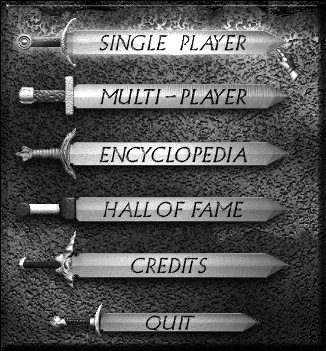
\includegraphics[width=0.4\textwidth]{SWmainmenu}
	\end{center}
	\vspace{-20pt}
\end{wrapfigure}

You will be taken to the Main Menu, where you will have a choice between playing a Single-Player or Multi-Player Game, or viewing the Encyclopedia or Hall of Fame. You also have the option to quit.

\subsection{Single-Player Game}

\index{game!single-player}

\textgoth{\Huge{I}}f you want to play a Single Player Game, \textbf{Click} on the Single Player Sword. When you do, you will bring up the following menu: 

\begin{center}
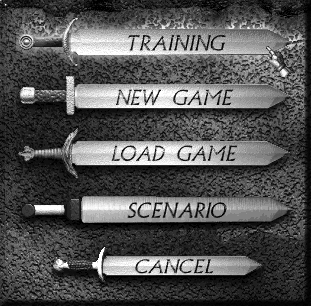
\includegraphics[width=0.5\linewidth]{SWsingleplayer}
\end{center}

\subsubsection{Training}

\textgoth{\Huge{I}}t is \textbf{\textit{strongly}} recommended that new players begin with the Training section. You may wish to go through all of the Training sessions even before reading the rest of this manual, which has been designed as an in-depth reference book.

When you \textbf{Click} on the Training Sword, you will be taken to a menu listing all of \textit{Seven Kingdoms: Ancient Adversaries} Training lessons.

\begin{center}
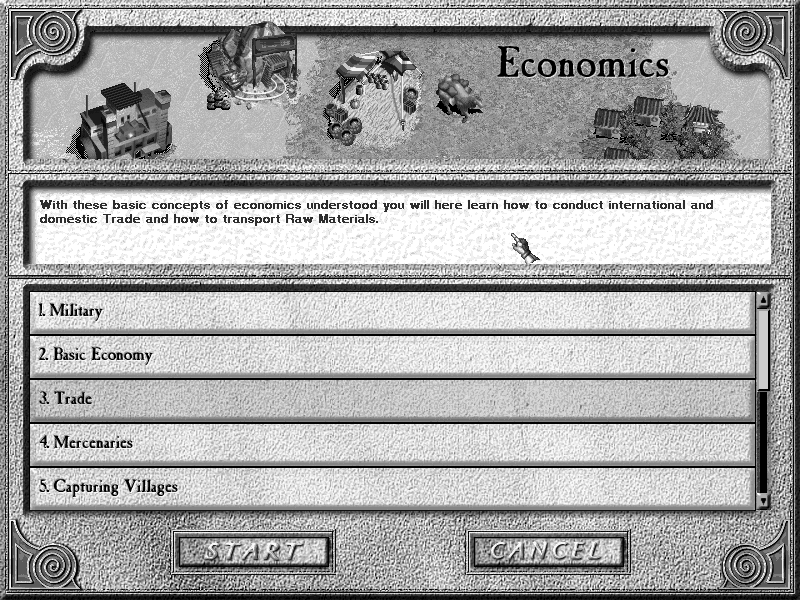
\includegraphics[width=0.9\linewidth]{Itraining}
\end{center}

% Not bold in original.

\textbf{IMPORTANT}: It is best if you take these lessons in order as later lessons will assume that you understand concepts presented previously.

When you \textbf{Click} on a topic you will see a brief description of the lesson. If you decide to proceed with the selected lesson, \textbf{Click} on the \textbf{Start Button}.

This will load a predesigned training scenario that will correspond to the chosen lesson.

The lesson text will appear at the top of your screen, leaving plenty of space for you to control the game below.

\begin{center}
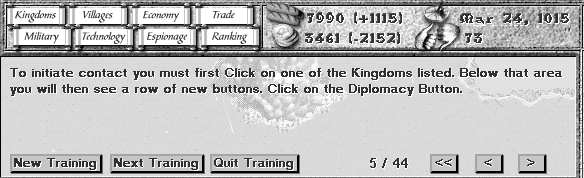
\includegraphics[width=0.9\linewidth]{Ilesson}
\end{center}

Page though the lessons by \textbf{Clicking} on the \textless and \textgreater \hspace{1pt} \textbf{Buttons} or do the same by pressing your \textless and \textgreater keys on your keyboard.

It is not strictly necessary that you learn your lessons within the designated training scenario. At any time during any Single Player game you may load a Training lesson if you wish to review any aspect of the game.

If you wish to proceed to the next lesson while remaining in the same game, \textbf{Click} on the \textbf{Next Training Button}.

To select a lesson that may not be the next in the series, \textbf{Click} on the \textbf{New Training Button}. This will return you to the menu where you can preview and select a different lesson.

\subsubsection{New Game}

\textbf{\textgoth{\Huge{C}}licking} on the New Game Sword will take you to the New Single Player Game options screens. Here you will see the four following Options pages:

\begin{center}
	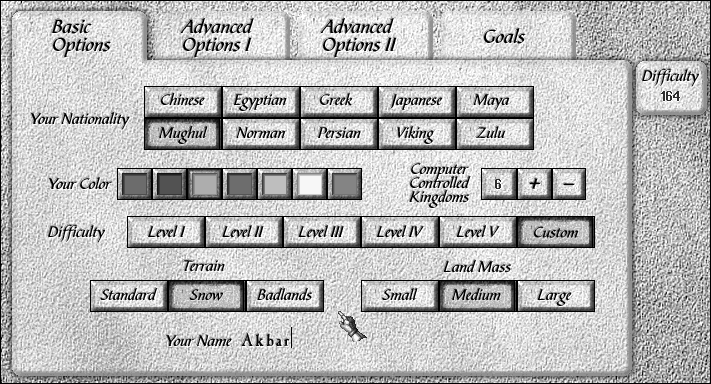
\includegraphics[width=0.9\linewidth]{Ibasicoptions}
\end{center}

On the \textbf{Basic Options} page, you may set your choices for your nationality, color, and the number of computer players.

Other options are also available below. Choose the level of difficulty at which you wish to play and then \textbf{Click} on that button. Level I is the generally the easiest and Level V the most difficult. Setting a level will automatically set corresponding options on the following Advanced Options I and II pages.

The final button, Custom, will be automatically set if you choose any options that do not match with the preset difficulty levels.

Two more options on this page are Terrain style and Land Mass. You will have three choices for each.

On the far right you can see an area with a number labeled “Difficulty”. This number will rise or fall depending upon the options that you set for the game. The maximum difficulty possible is 200. This difficulty number will be used to determine your final score---a higher difficulty rating means that the possible range of scores will be higher as well.

On the bottom of this options page there is space for you to type in your name. This name will be used by your King at the start of the game.

On the \textbf{Advanced Options I} page you will find the following options:

\begin{center}
	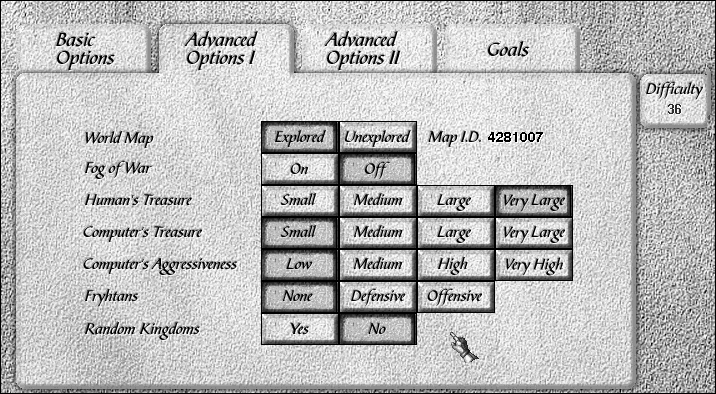
\includegraphics[width=0.9\linewidth]{Iadvancedoptions1}
\end{center}

\textbf{World Map}: Here you may choose whether the world will be unexplored at the start of the game, or completely explored with all map features visible.

\begin{changemargin}{0.5cm}{0cm} 
 \textbf{The Map I.D.} is the random-number seed from which your new world map will be generated. If you wish to play with a map that you particularly enjoyed from a previous game, you may enter its number by typing it in on your keyboard. Do not enter the commas that separate the numbers. They are there to make the number easier to read.
\end{changemargin}

\begin{changemargin}{0.5cm}{0cm} 
 If you have already begun a game and wish to check on the Map I.D., \textbf{Click} on the \textbf{Menu Button} at the top right of your screen. The Map I.D. will be on the bottom of the Menu area.
\end{changemargin}

\textbf{Fog of War}: Here you decide whether there is a limit to the distance your units can see (On) or if you will be able to see all activity in the world at any time (Off).

\textbf{Human’s Treasure}: Sets the amount of money with which you will begin the game.

\textbf{Computer’s Treasure}: Sets the amount of money with which your computer foes will begin the game.

\textbf{Computer’s Aggressiveness}: Sets whether your computer-controlled rivals are passive or aggressive.

\textbf{Fryhtans}: This will determine if Fryhtans are a part of the game or not, and if they are, whether they will only fight to defend themselves, or if they may attack on their own initiative.

\begin{changemargin}{.5cm}{0cm}
If set to Defensive, the Fryhtans will remain in their Lairs unless attacked.

If set to Offensive, Fryhtans may attack on their own, especially if a village is settled or a building built too near to their Lair. 

They will also expand their numbers by planting new Lairs around the land.
\end{changemargin}

\textbf{Random Kingdoms}: When this option is turned On, the computer will randomly choose the nationalities of other Kingdoms in the game. It is quite possible, in this case, that other Kingdoms will be of the same nationality as your own. This can make for very interesting games as you vie for control of Independent Villagers who share your nationality.

This setting will also randomize each Kingdom’s initial Village population, including your own. A small population will be somewhat offset by granting a few skilled, mobile units at the start of the game.

\begin{center}
	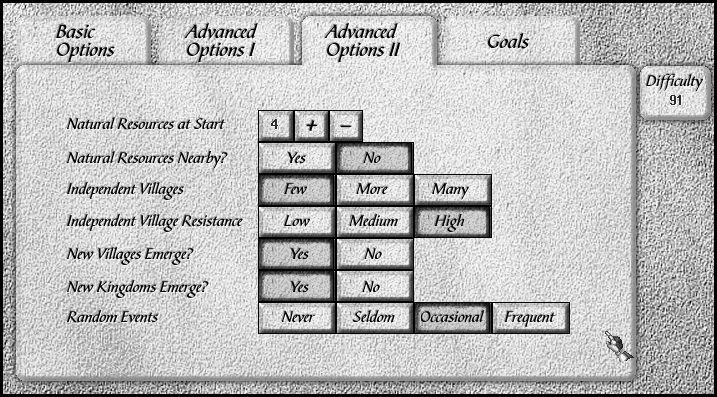
\includegraphics[width=0.9\linewidth]{Iadvancedoptions2}
\end{center}

On the \textbf{Advanced Options II} page you will find still more options. These are as follows:

\textbf{Natural Resources at Start}: This number, between 1 and 7, will set how many Natural Resources will be spread throughout the world at the start of the game.

\textbf{Natural Resources Nearby?}: This option determines whether or not each kingdom will have a Natural Resource deposit automatically located near its starting village.

\textbf{Independent Villages}: This sets the approximate number of Independent Villages.

\textbf{Independent Village Resistance}: This sets the level of resistance to your rule for all of the Independent Villages. It also influences the Combat abilities of Independent units.

\textbf{New Villages Emerge?}: This determines whether or not new Independent Villages may be settled during the game.

\textbf{New Kingdoms Emerge?}: This determines whether or not new Kingdoms may be founded after the destruction of old ones.

\textbf{Random Events}: This sets the frequency of random natural disasters such as earthquakes, lightning strikes, and tornadoes---all of which can cause damage to buildings and injury to units.

\begin{center}
	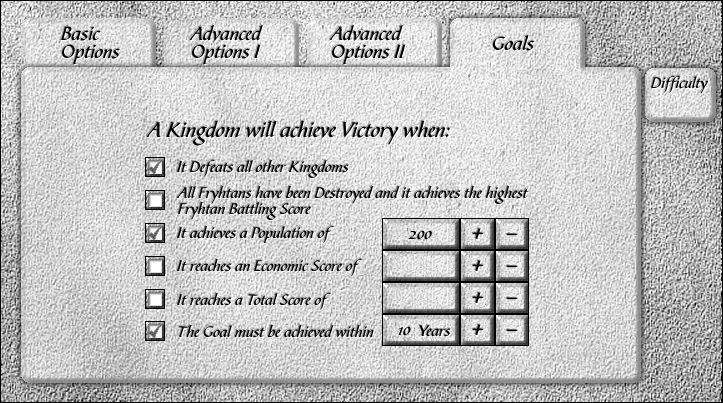
\includegraphics[width=0.9\linewidth]{Igoals}
\end{center}

On the \textbf{Goals} page, you will be able to define the victory conditions for your game. The first kingdom to achieve any of the chosen goals will be the winner.

These goals include the following:

\textbf{Defeat All Other Kingdoms}: This is not an option. Defeating all other kingdoms always results in victory, because it eliminates any possible competition for other goals. If no other goals are chosen, then victory cannot be achieved without eventually destroying all rivals, even those with whom you may have developed friendships and alliances.

\textbf{Destroy All Fryhtans}: Ridding the world of these vile creatures is a goal that all kingdoms will happily work toward. After the last of them has been destroyed, the kingdom which has dispatched the most Fryhtans will be the winner.

You may view your current score in Fryhtan Battling by \textbf{Clicking} on the Ranking Scroll at the top of your game screen.

\textbf{Achieve a Population of..}: This may seem a peaceful goal, but it can often be achieved only through taking Villages by force.

\textbf{Reach an Economic Score of..}: Even the lowest possible goal here of 100 will not be achieved unless you are prepared to defend yourself and to take and hold more than one Village and, of course, to prevent your enemies from doing the same. You may check your Economic Score and the scores for the other Kingdoms by \textbf{Clicking} on the Ranking Scroll at the top of your screen and then \textbf{Clicking} on the name of the Kingdom that you want to check. Their Economic Score will appear in the box below.

\textbf{Reach a Total Score of..}: Achieving this goal requires a balanced approach to the rulership of one’s kingdom. You may check on your Total Score and that of your rivals in the same way that you checked the Economic Score.

\textbf{Achieve Goal Within..}: This will set a deadline for the achievement of the above goals.

\subsection{Winning and Losing}

\textgoth{\Huge{Y}}ou will win the game if you achieve any of the chosen goals and, if you have set a time limit, done it before that time limit is reached.

It may come to pass that, having set as your goal something other than the defeat of all of the other Kingdoms, you find a way to destroy all of your rivals anyway. Defeating all other kingdoms is always one of the goals, so you will still win the game in such a case, because the last of your competition has been eliminated.

You will lose the game if your Kingdom is destroyed, if another Kingdom has achieved a set goal, if you have failed to achieve your goal in the set time, or if you have surrender to another Kingdom.

Even though you have lost, you may continue to observe the progress of the game. The game will continue to run until you decide to either Quit or to Retire, although the score of such a game will be ineligible to be entered in the Hall of Fame.

\subsubsection{Load Game} % Lots of whitespace below

\index{game!loading previous saved}

\textbf{\textgoth{\Huge{C}}licking} on the Load Game Sword will take you to the Load Game menu where you can scroll up and down to see any games that you have previously saved.

\begin{center}
	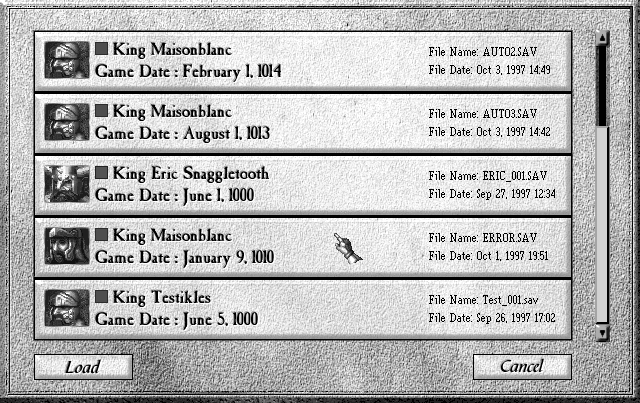
\includegraphics[width=0.9\linewidth]{Iload} % 0.7 reduces whitespace.
\end{center}

To load a game, \textbf{Click} on its Bar and then \textbf{Click} on the \textbf{Load Button}. You may also \textbf{Double-Click} on the Bar.

Single Player Games will have the .SAV file extension. Multiplayer Games will have the .SVM extension.

\subsubsection{Scenario}

\index{game!scenarios}

\begin{center}
	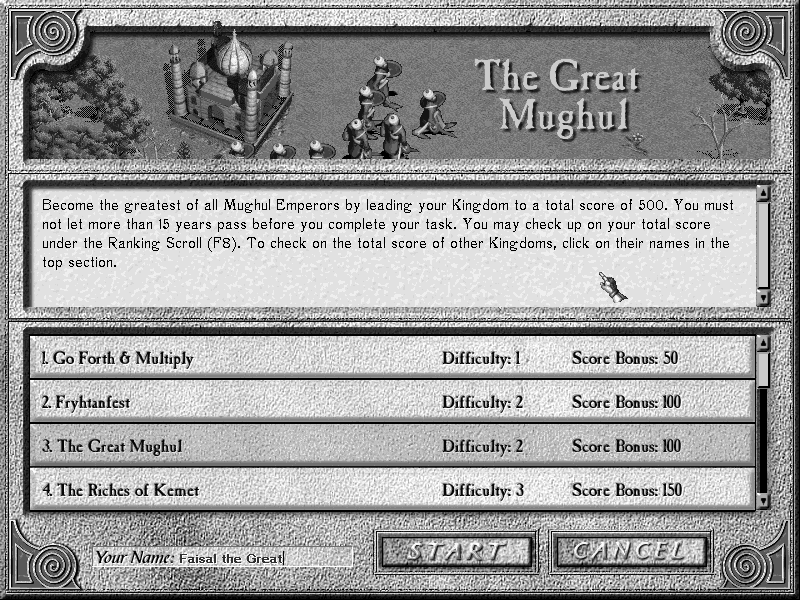
\includegraphics[width=0.9\linewidth]{Iscenario} % 0.7 reduces whitespace.
\end{center}

\textgoth{\Huge{C}}hoosing to play a Scenario will take you to a menu similar to the one for choosing a Training lesson. \textbf{Click} on the Scenario that you wish to play. You will see a brief description of the beginning situation and the goal(s) to be achieved. When you are ready to begin, \textbf{Click} on the \textbf{Start Button}.

\subsection{Multiplayer Game}

\index{game!multiplayer}

\begin{center}
	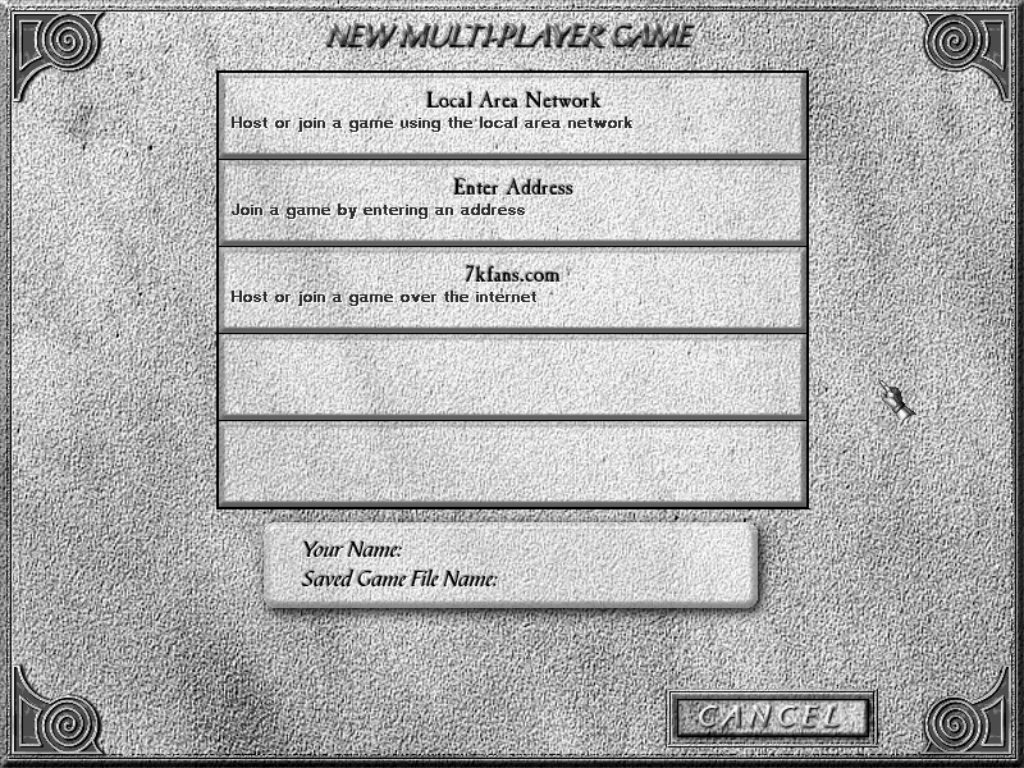
\includegraphics[width=0.9\linewidth]{Imultiplayer}
\end{center}

\subsubsection{Initial Setup} % wiki content. Author?

\textgoth{\Huge{A}}ll players need the same version of the game, or compatibility issues will arise. Allow \textit{Seven Kingdoms: Ancient Adversaries} to pass through your firewall. If you have a router, port forwarding may be needed. 2.14.7+ uses UDP port 19383 for LAN and 7kfans.com game browsing.

\subsubsection{Lobby}

\textgoth{\Huge{W}}hen you \textbf{Click} on the multiplayer Sword you will see three connection options: Local Area Network, Enter Address (Direct IP), and 7kfans.com. \textbf{Click} on the type of connection that you will be using.

On the bottom, enter your name just as you would in a Single Player Game. This will be used by your King at the start of the game.

Beneath your name, you will see the name of the game. You will be able to save one multiplayer game only. Its name will be MULTI. You may not change this name.

There will also be two auto-saved games, named AUTO01.SVM and AUTO02.SVM. One of them will have a later date than the other, so you will know which is the most recent.

To load a saved game, Select the name of your save game file and \textbf{Click} on Load (everyone must select the same file; "Game Date" must be the same).

\subsubsection{7kfans.com}

\textgoth{\Huge{I}}f you are setting up the game, \textbf{Click} on the \textbf{Create Button}. If someone else is setting up the game, \textbf{Click} on the \textbf{Join Button}. To return to the previous screen, \textbf{Click} on the \textbf{Cancel Button}.

\begin{center}
	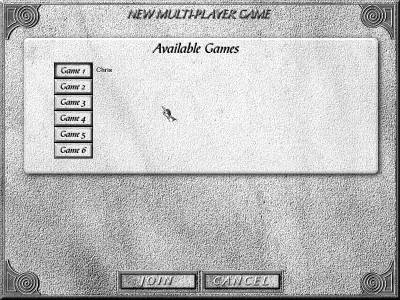
\includegraphics[width=0.9\linewidth]{Imultiplayer2}
\end{center}

If you are not creating this game, a \textbf{Click} on the \textbf{Join Button} which will send you to the Available Games page.

You will be prompted to enter your forums account username and password. If you have recently logged into the forums, you may leave your password empty.

There you will find a list of the games that have been created. They will be listed by the name the creator set. The default session name is the creator’s username. It may take a few seconds for the list of games to appear.

\textbf{Click} on the desired game’s name. Then \textbf{Click} on the \textbf{Join Button} on the bottom of the page. This will take you to the multiplayer Options pages.

\subsubsection{Enter Address}

\textgoth{\Huge{I}}f you are hosting the game, \textbf{Click} on the \textbf{Create Button}. Set the session name and choose a password. You may choose to leave the password blank. Use your external IP address to let players connect. Wait for players to join. If you are joining a game, \textbf{Click} on the \textbf{Join Button}. Enter the IP address of the host. This will take you to the multiplayer Options pages.

\subsubsection{Local Area Network}

\textgoth{\Huge{I}}f you are creating the game, \textbf{Click} on the \textbf{Create Button}. If you are joining the game, \textbf{Click} on the \textbf{Join Button}. This will take you to the multiplayer options pages.

\subsubsection{Multiplayer Options}

\textgoth{\Huge{T}}he multiplayer Options will be the same as the ones that you saw in the Single Player Options. The creator of the game sets most of the options. If you are joining a game created by someone else, you may only choose your nationality and your color.

% Graphic is right justified not centered in original.

\begin{center}
	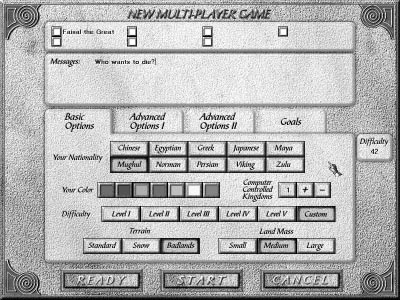
\includegraphics[width=0.9\linewidth]{Imultiplayer3}
\end{center}

The multiplayer options page includes a list of players who have joined the game, and a Chat window where players may discuss options selection, strategy, or how they intend to grind their rivals into dust. These items do not appear on the Single Player Options screen.

To send a message in the Chat window, simply type anything that you want to say. When you have finished typing, press the Enter key on your keyboard. Your message will then be posted for the other gamers to see.

Once you have set all of your options and \textbf{Clicked} on the \textbf{Ready Button}, a red check mark will appear next to your name. Do not \textbf{Click} next to your name. Nothing will happen. When every player has a red check mark visible, the creator of the game will be able to \textbf{Click} on the \textbf{Start Button} and begin the game.

\subsubsection{Matchmaking}

\textgoth{\Huge{Y}}ou can post or search on the Forums to look for other players or set up matches. Look for the matchmaking thread. There are additional resources for people looking to play multiplayer such as contact information of other players.

\subsection{Encyclopedia}

\index{encyclopedia}

\begin{center}
	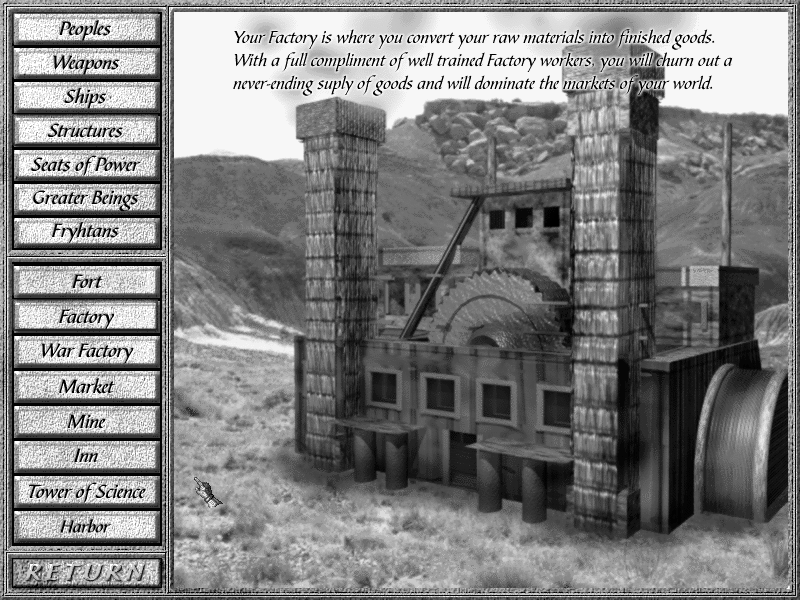
\includegraphics[width=0.9\linewidth]{Iencyclopedia} % Circa
\end{center}

\textgoth{\Huge{T}}he Encyclopedia includes images and informative descriptions of units and buildings appearing in \textit{Seven Kingdoms: Ancient Adversaries}.

\textbf{Click} on one of the titles in the top section. When you do you will see listed in the bottom section a group of subjects that are under that title.

When you \textbf{Click} on one of these you will see a picture and description of that subject.

If you do not \textbf{Click} on anything, the Encyclopedia will present you with a slideshow of all of its subjects.

\subsection{Hall of Fame}

\textgoth{\Huge{A}}t the end of every game of \textit{Seven Kingdoms: Ancient Adversaries} your score will be computed. Your score will take into account the difficulty level at which you were playing and the skill with which you played.

If your final score is one of the six highest ever recorded, it will be entered into the Hall of Fame.

\subsection{New Game}

\begin{wrapfigure}{r}{0.5\textwidth}
	\begin{center}
		\vspace{-20pt}
		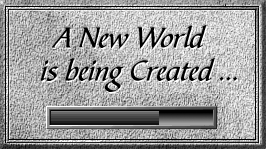
\includegraphics[width=0.4\textwidth]{Inewworld}
	\end{center}
\vspace{-20pt}
\end{wrapfigure}

\textgoth{\Huge{E}}very time you play a new game, a completely new world will be generated at random, giving you a nearly limitless number of worlds to subject to your will.

As soon as the new world’s lands have been separated from its waters and its mountains have been raised, you will be given a small village to call your own. From these humble beginnings you must do your best to survive and to prosper through a combination of exploration, training, construction, trade, espionage, diplomacy, and armed conflict.

You will need to develop a variety of skills to be an effective leader, and to command the loyalty of your people. Standing in your way will be other kings, evil Fryhtans, and the ravages of nature itself.

\section{Main Menu}

\textgoth{\Huge{W}}hile you are playing a game of \textit{Seven Kingdoms: Ancient Adversaries}, you will be able to access various options by \textbf{Clicking} on the \\ % FIXES AN OVERFLOW
\textbf{MENU Button} at the top right of your screen. This will bring up the options as seen below.

% Graphic is right justified not centered in original.

\begin{center}
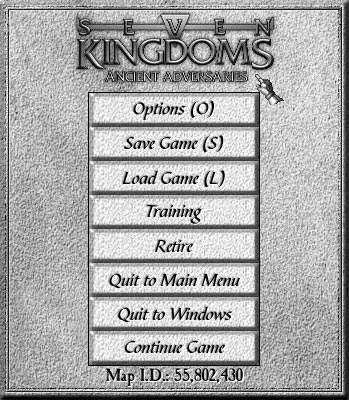
\includegraphics[width=0.5\linewidth]{Imainmenu}
\end{center}

\subsection{Options}

\textgoth{\Huge{T}}he first choice you will have, which can also be accessed by pressing the O key on your keyboard, is the In-game Options Page.

\begin{center}
	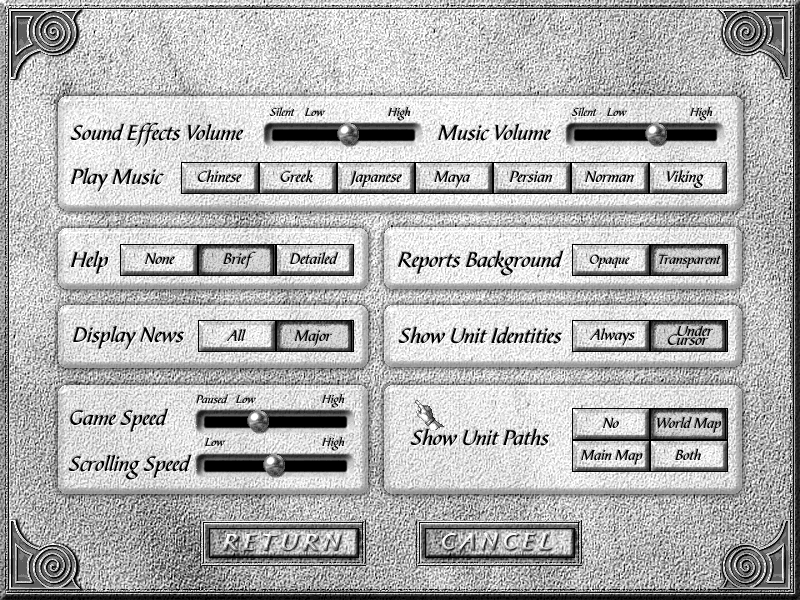
\includegraphics[width=0.9\linewidth]{Ioptions}
\end{center}

Here you can set your Sound Effects and Music volume. Do this by sliding the brass ball left or right until it is in the position that you want.

You may also choose to play any single piece of \textit{Seven Kingdoms: Ancient Adversaries} music.

You can set the detail level of pop-up instructional text that will appear whenever you hold the cursor over a button or icon for a few seconds. You may also turn this feature off, if you prefer.

You can choose to view all News items or only the most important ones.

You can set the Speed of the game (which can also be set on your keyboard by pressing the 0–-9 keys at any time) and the Scrolling Speed of your screen.

For your Reports Background you have the option of seeing through them to any action that is taking place (transparent), or the option of making them opaque.

Unit Identities (what kind of skills units possess) can be set to be seen at all times or only when a unit is under your cursor.

Finally, you may whether to display the projected Paths that your units will take when they have been ordered to move to a different part of the map.

\subsubsection{Help}

\textgoth{\Huge{T}}o use the Help function, simply hold your cursor over any button or icon in the game. After a few seconds, a display will appear explaining the use of the button or meaning of the icon. You may set the detail level of this Help function on the Options Page (O), or disable it if you prefer.

Because the Help function pauses the game momentarily to allow you time to read, it will not be available in multiplayer games.

\subsection{Save Game}

\index{game!saving}

\textgoth{\Huge{I}}f you choose Save Game, you will be presented with a screen showing all of the games that have previously been saved. You may choose to overwrite any one of these games by \textbf{Clicking} on the game’s name and then \textbf{Clicking} on the \textbf{Save Button}.

\begin{center}
	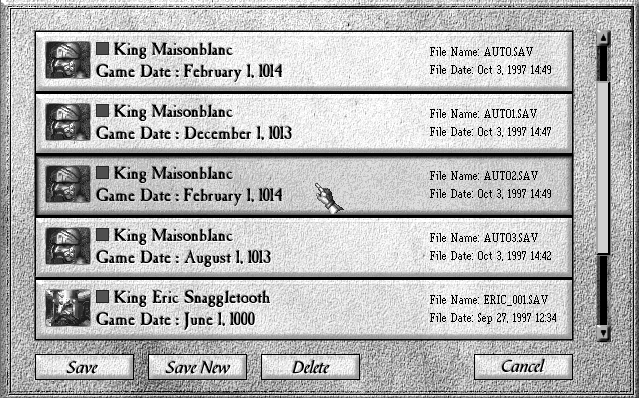
\includegraphics[width=0.9\linewidth]{Isavegame}
\end{center}

You may also choose to save your game in a new file by \textbf{Clicking} on the \textbf{Empty Game Slot Button}, which will be at the very top of the list, and then on the \textbf{Save New Button}.

\begin{center}
	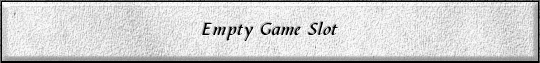
\includegraphics[width=0.7\linewidth]{Isavegame_emptyslot}
\end{center}

Although the number of games that you can save is limited only by your disk space, you may wish to delete some of your more humiliating defeats. To do so, \textbf{Click} on the game and then \textbf{Click} on the \textbf{Delete Button}.

The game that you are playing will be automatically saved in a separate file after every two months of game time. Auto-saved games will have filenames beginning with AUTO.

\subsection{Retire}

\textgoth{\Huge{W}}hen you decide to retire from a game of \textit{Seven Kingdoms: Ancient Adversaries}, the game will end and your score will be calculated.

If you have achieved a high enough score, it will be entered in the Hall of Fame.

If you choose to Retire from a multiplayer game, the computer will take control of your kingdom and do its best to finish on top.

\subsection{Map I.D.}

\textgoth{\Huge{T}}he Map I.D. is the random number seed from which your present world map was generated. Make a note of this number if you particularly like a random map and would like to use it again, share it with your friends, or post on the Internet.

\section{Mouse and Keyboard Commands and Cheat Codes}

% i think one or two is missing: new kingdom emerge, replay.

\subsection{Mouse Commands}

\begin{center}
	\begin{tabular}{|p{2in}|p{2in}|}
		\hline
		Action	& Description \\ \hline
		Click	& Press the left mouse button once. \\ \hline
		Double-Click	& Press the left mouse button twice quickly. \\ \hline
		Right-Click	& Press the right mouse button once. \\ \hline
		Group Select	& Click and hold down the left mouse button, dragging a box around the intended group. \\ \hline
		Right-Click on town transfer	& Transfers 10 peasants \\ \hline
		Right-Click on research project	& Sets research project for all towers of science \\ \hline
		Right-Click on train unit	& Dequeue 8 units \\ \hline
		Right-Click on collect tax	& Set automatic tax \\ \hline
		Right-Click on grant	&  Set automatic grant \\
		\hline
	\end{tabular}
\end{center}

\clearpage

\subsection{Keyboard Commands}

\begin{center}
	\begin{tabular}{|p{1in}|p{3in}|}
		\hline	 
		Action	& Description \\ \hline
		Esc	& Close Scroll Reports. \\ \hline
		F1	& Kingdoms report \\ \hline
		F2	& Villages report \\ \hline
		F3	& Economy report \\ \hline
		F4	& Trade report \\ \hline
		F5	& Military report \\ \hline
		F6	& Technology report \\ \hline
		F7	& Espionage report \\ \hline
		F8	& Ranking report \\ \hline
		F9	& View the News Log. \\ \hline
		F11	& Capture the Screen to a .BMP file. The screenshot will be saved in the game’s directory. \\ \hline
		0 (zero) & Pause the Game. Many overlays and menus will still be operational even while the game is paused. Units can be given new orders, but they will carry them out when the game is resumed. \\ \hline
		1--9 & Set the Speed of the Game. 1 is the slowest---and 9 the fastest. \\ \hline
		Spacebar & Pause/unpause the game. \\ \hline
		Shift + Right-Click	& Queue 8 units / queue 10 weapons / queue 4 ships \\ \hline
		Up / Down Arrows & Go to the previous/next building of the same type as the currently selected one. \\ \hline
		Left / Right Arrows	& Go to the previous/next object of the same type and of the same nationality as the currently selected one. \\ \hline
		b & If you select a unit, it will give you the build command. If you select a town, it will give you the train command. \\ \hline
		b+a	& Build a factory \\ \hline
		b+f	& build a fort \\ \hline
		b+h	& build a harbor \\ \hline
		b+i	& build an inn \\ \hline
		b+m	& build a market \\ \hline
		b+p	& build a seat of power \\ \hline
		b+r	& build a mine \\ \hline
		b+t	& build a tower of science \\ \hline
	\end{tabular}
\end{center}

\begin{center}
	\begin{tabular}{|p{1in}|p{3in}|}
		\hline	 	
		Action	& Description \\ \hline
		d	& Open first diplomacy message / reply to chat \\ \hline
		e	& Switch the World Map Display Modes. \\ \hline
		f	& Select a Fort and center the screen on it. Press repeatedly to cycle through all of your Forts. Pressing the left or right arrow keys will also cycle through your Forts. Pressing the up and down arrow keys will cycle through all Forts, including those of other Kingdoms. \\ \hline
		g	& Select a General and center the screen on him. Press repeatedly to cycle through all of your Generals. \\ \hline
		u	& Select a Ship and center the screen on it. Press repeatedly to cycle through all of your Ships. \\ \hline
		j	& Center the screen on the location of a Natural Resource deposit. \\ \hline
		k	& Select your King and center the screen on him. \\ \hline
		l (el)	& Load a Game. \\ \hline
		o (oh)	& In-Game Options Menu. \\ \hline
		p	& Toggle between Opaque and Transparent Reports. \\ \hline
		r	& If you select a fort, it will Sortie the soldiers. If you select soldiers, it will withdraw them. If you select a village, it will recruit peasants. \\ \hline
		s	& Save the Game. The game will be Auto-Saved every two months in a separate file. \\ \hline
		t	& Settle \\ \hline
		x	& Clear all News and / or Chat messages from the screen. \\ \hline
		y	& Select a Spy and center the screen on him. Press repeatedly to cycle through all of your Spies. \\ \hline
	\end{tabular}
\end{center}	

\begin{center}
	\begin{tabular}{|p{1in}|p{3in}|}
		\hline	 	
		Action	& Description \\ \hline
		\textgreater & Next block of text in Training. \\ \hline
		\textless	& Previous block of text in Training. \\ \hline
		Ctrl + (0--9)	& Assign all selected units to a numbered group. \\ \hline
		Alt + (0--9)	& Select all mobile units previously assigned to a numbered group. \\ \hline
		Alt + Right-Click	& Manually assign waypoints to mobile unit(s). After setting waypoints, use a normal Right Click to set the final destination. \\ \hline
		Alt + Enter & Enter or leave windowed mode \\ \hline
		Alt + g & Screen grab in windowed mode \\ \hline
		Alt + F4	& Quit to Desktop \\ \hline
	\end{tabular}
\end{center}

\subsection{Cheat Codes}

\textgoth{\Huge{T}}ype !!!@@@\#\#\# during gameplay to enable cheat mode. Note that the game will say you cheated, and your score will be zero.

\begin{center}
	\begin{tabular}{|p{1in}|p{3in}|}
		\hline	 
		Action	& Description \\ \hline
		c	& Add \$1000 \\ \hline
		n	& Add all technology \\ \hline
		u	& Enable / disable King immortal mode. \\ \hline
		z	& Construct building instantly \\ \hline
		=	& Fill prayer bar in seat of power \\ \hline
		[	& +20 combat skill \\ \hline
		]	& +20 skill \\ \hline
		;	& +10 population \\ \hline
		‘	& +20 spy skill \\ \hline
		\textbackslash & Add 1000 food \\ \hline
		/	& Reveal map \\ \hline
	\end{tabular}
\end{center}
%*
%* Seven Kingdoms: Ancient Adversaries
%*
%* Copyright 1997,1998 Enlight Software Ltd.
%* Copyright 2018 Timothy Rink
%*
%* This program is free software: you can redistribute it and/or modify
%* it under the terms of the GNU General Public License as published by
%* the Free Software Foundation, either version 2 of the License, or
%* (at your option) any later version.
%*
%* This program is distributed in the hope that it will be useful,
%* but WITHOUT ANY WARRANTY; without even the implied warranty of
%* MERCHANTABILITY or FITNESS FOR A PARTICULAR PURPOSE.  See the
%* GNU General Public License for more details.
%*
%* You should have received a copy of the GNU General Public License
%* along with this program.  If not, see <http://www.gnu.org/licenses/>.
%*
%*

\chapter{The Information Interface}

\index{game!interface}

On the top of your screen, you will see all of the information necessary to keep your budding Empire under your firm grip.

\begin{center}
	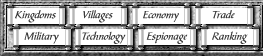
\includegraphics[width=0.7\linewidth]{Iscrolls}
\end{center}

Beginning on the Left, you will see the Scrolls. \textbf{Click} on a Scroll to see the detailed information inside each. You may also access these Scrolls by pressing the \textbf{F1} through \textbf{F8} keys on your keyboard.

Once you have opened one of these Scrolls, it can be closed by \textbf{Clicking} it again or by pressing the \textbf{Esc} key on your keyboard.

\section{Kingdoms}

Open this Scroll if you want to see information on all of the world’s Kingdoms that you have discovered so far in your explorations of the world.

\begin{center}
	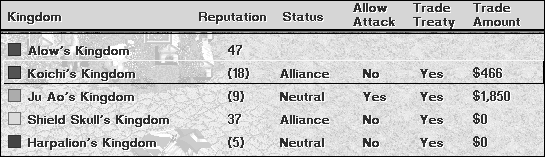
\includegraphics[width=0.7\linewidth]{Ikingdoms}
\end{center}

Below this area, you will see three buttons that will take you into three different areas. These are \textbf{Information}, \textbf{Diplomacy}, and the \textbf{Diplomatic Log}.

\subsection{Information}

Under the \textbf{Information Button}, you will see more detailed information on your relationship with the selected Kingdom.

\begin{center}
	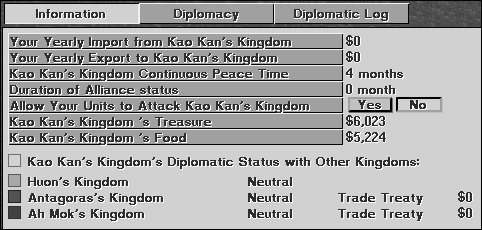
\includegraphics[width=0.7\linewidth]{Ikingdoms_information}
\end{center}

You will also be able to see the diplomatic relationships that the other Kingdoms have with each other.

For Kingdoms that are your allies, you will be able to see their cash and food reserves as well.

The Yearly Imports and Exports are figured for the preceding 365 days.

\subsubsection{Allow Attack}

\index{allowing attack}

By \textbf{Clicking} the \textbf{Yes} or \textbf{No Buttons} in this section, you will be able to manually select whether or not your troops will be allowed to attack units or structures of the selected Kingdom. The game will begin with the default setting of Yes.

The Yes or No option will be set automatically in the following situations:

\begin{adjustwidth}{1cm}{}

\index{attacking!Allow Attack option}
	
When you form a Friendly or Alliance Treaty with another Kingdom, your Allow Attack option will be automatically set to No. You will be unable to attack any units or structures unless you manually change the setting.

When you enter into a War with a Kingdom, your Allow Attack option will be automatically set to Yes.

If you accept a Cease Fire in a war, the Allow Attack option with the other signatory will be changed to No.
\end{adjustwidth}

It would be very wise of you to set the Allow Attack option to No for every Kingdom that you are not planning to attack. This will prevent the sometimes unavoidable incidents of friendly-fire casualties from blowing up into full-scale war. If Allow Attack is set to No, the other Kingdom will understand that any such incident was just a mistake.

\subsection{Diplomacy and Diplomatic Log}

For these two buttons, see the detailed descriptions in \textbf{Chapter 13}.

\section{Villages}

Opening this Scroll will give you detailed information on all of your Villages. This includes Village Population, the number of Peasants, Village Loyalty, and a list of the various Nationalities living in the Village.

\textbf{Double-Clicking} on the name of a Village will center it on your screen.

In the bottom chart, you will see a detailed list of your Buildings, including their Building Cost, Number, Yearly Upkeep Cost, and Yearly Income (if any) from that Building. The “Yearly” figures are based on the past 365 days.

\section{Economy}

\index{economy scroll}

Open this Scroll to see all the information you could wish for on your economy. It will detail all of your income and expenses and the Profit or Loss that you are running at the present time. This includes:

\subsection{Income}

\index{income}

\subsubsection{Sale of Goods}

The amount of sales of Finished Goods to Villagers.

\subsubsection{Exports}

The amount of exports of Raw Materials or Finished Goods to other Kingdoms.

\subsubsection{Taxes}

The amount of Taxes collected from Villagers.

\subsubsection{Recovered Treasure}

The amount of Treasure recovered from the slaying of Frhytans.

\subsubsection{Worker Income}

The income received by your subjects who are working in the firms of other Kingdoms.

\subsubsection{Sale of Buildings}

Your income from the sale of your Factories, Mines, Towers of Science, etc.

\subsubsection{Tribute from other Kingdoms}

Money that you have either forced other Kingdoms to pay you or that they have given in hope of obtaining your good will.

\subsection{Expenses}

\index{expenses}

\subsubsection{General Costs}

The Maintenance costs for all of your Generals.

\subsubsection{Spy Costs}

The Maintenance costs for all of your Spies.

\subsubsection{Other Mobile Human Unit Costs}

The Maintenance costs for all human units except Generals and Spies.

\subsubsection{Caravan Costs}

The Maintenance costs for all of your Caravans.

\subsubsection{Weapons Costs}

The Maintenance costs for all of your Weapons.

\subsubsection{Ships Costs}

The Maintenance costs for all of your Ships.

\subsubsection{Buildings Costs}

The Construction and Maintenance costs for all of your Buildings.

\subsubsection{Training Units}

The Cost of Training all of your units.

\subsubsection{Hiring Units}

The Cost of Hiring units from Inns.

\subsubsection{Honoring Units}

The Cost of Honors given to your units.

\subsubsection{Foreign Worker Salaries}

The money paid to foreigners working in your Buildings.

\subsubsection{Grants to your Villages}

The Cost of your Grants to your Villages.

\subsubsection{Grants to other Villages}

The Cost of your Grants to other Villages.

\subsubsection{Imports}

The Costs of all of your Imports.

\subsubsection{Aid/Tribute to other Kingdoms}

The Money that you have paid in Tribute or given in Aid to other Kingdoms.

\section{Trade}

\index{trade scroll}

Inside this Scroll you will see detailed the routing and loads of all of your Caravans and all of your Ships that are being used in Trade. \textbf{Double-Clicking} on a Caravan or a Trader in this menu will center your screen over it.

\section{Military}

\index{military scroll}

In this Scroll, you will see your military disposition. It will list your King and all of your Generals and the number of troops that they command. \textbf{Double-Clicking} on the King or a General will center your screen over his location.

\section{Technology}

This Scroll reports on the progress of all of your research projects in all of your Towers of Science.

It also shows the Scrolls of Power that you have acquired and your Greater Beings that are currently active.

\section{Espionage}

\index{espionage scroll}

This top-secret Scroll details the activities of all of your spies all over the world. \textbf{Double-Clicking} on a spy’s listing will center the screen over his location.

\section{Ranking}

\index{ranking scroll}

This Scroll will show you the rank of your Kingdom against all of the other Kingdoms in a number of categories, such as Population, Military Strength, Economic Strength, Reputation and Fryhtan Battling.

It will also give you a total score by adding up these different categories, show all set Goals and display the total playing time.

\section{State of the Kingdom}

\index{kingdom!state of}

\begin{center}
	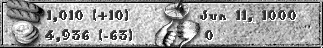
\includegraphics[width=0.7\linewidth]{Ifoodgoldetc}
\end{center}

To the right of the Function Scrolls, you will see four icons. These are, on the left: Food and Treasure, and on the right: Date and Reputation.

\subsection{Food}

\index{food}

The number in the upper left indicates how much Food is stored in your empire. The number in the parentheses to the right shows how much of a food surplus or deficit you have produced in the past year.

Each person in your kingdom, whether a Peasant, Worker or Mobile Unit, consumes 10 units of food each year. Remember that food is produced by your Peasants. If you do not keep enough Peasants you will run out of food. To maintain a constant food supply, you will need one Peasant toiling in the field for every three subjects of your kingdom.

If your Kingdom runs out of food, prepare for the worst. The Loyalty Levels of all of your units will decrease by one point every five days.

You may request to purchase food from other Kingdoms under the \textbf{Kingdoms Scroll/Diplomacy Button menu}.

\subsection{Treasure}

\index{treasure}

The number in the lower left indicates the amount of gold in your treasury. The number in the parenthesis to the right shows how much of a cash surplus or deficit you have incurred in the past year.

It is very important to keep your eyes on your Treasury and your Food supply.

Without money to pay the salaries of your Generals or Mobile units you will see a decrease in their Loyalty.

If you don’t have enough to pay your Spies in foreign Kingdoms, their Loyalty will also decrease. If they are acting as Counterspies in your own Kingdom you will also need to feed them. If you cannot their Loyalty will decrease.

If you can no longer pay foreign workers, they will resign.

If you no longer have enough money to maintain your Weapons or Ships, they will begin losing Hit-Points. If the situation continues, they will completely break down.

If you run out of funds, you will no longer be able to maintain your buildings. They will fall into disrepair and eventually collapse.

\subsection{Calendar}

\index{calendar}

It is here that you see the day and year. In a multiplayer game, this may become very important when you and your Allies are synchronizing an attack on another Kingdom.

\subsection{Reputation}

\index{reputation}

This number represents the esteem in which your Kingdom is held by the people of the world. A high Reputation level can have many and varied benefits during the long struggle for world domination.

Your Reputation may suffer if you persist in actions that other Kingdoms find to be downright antisocial or if you fail to adequately protect your subjects. The following are the various penalties you will pay for your behavior:

\begin{adjustwidth}{1cm}{}
If you attack a Kingdom without first declaring war:

Your Reputation will decrease by 40\% of your target’s Reputation, but only if the target has a positive Reputation.

\textbf{If you declare war on another Kingdom:}

Your Reputation will decrease by 20\% of your target’s Reputation, but only if the target has a positive Reputation.

\textbf{If you terminate an alliance treaty:}

Your Reputation will decrease by 20\% of the target’s Reputation, but only if their Reputation is positive. Note that if you declare war on an ally, your Reputation will decrease twice: once for declaring war and once for terminating an alliance.

\textbf{If you terminate a friendly treaty: }

Your Reputation will decrease by 10\% of the target’s Reputation, but only if the target has a positive Reputation. Note that if you declare war on a Kingdom with which you have a friendly treaty your Reputation will decrease twice; once for declaring war and once for terminating a friendly treaty.

\textbf{If you terminate a trade treaty:}

Your Reputation will decrease by 5\% of the target’s Reputation, but
only if the target has a positive Reputation.

\textbf{Additional Penalties}

\textbf{-10} points for destroying an enemy Caravan.

\textbf{-10} points for Sinking a Trader.

Although Caravels and Galleons may be used for trade, they are armed and may, therefore, be sunk without penalty.

\textbf{-3} points if one of your Caravans is destroyed by an enemy.

\textbf{-3} points if one of your Traders is sunk by an enemy.

\textbf{-3} points if one of your Spies is caught Spying.

\textbf{-1} points for each enemy Civilian collaterally damaged in the defense of their town.

\textbf{-0.3} points for each enemy Civilian collaterally damaged in battle.

\textbf{-0.3} points if one of your Civilians is cruelly murdered by an enemy.

Your Reputation will automatically increase by \textbf{+0.5} points per month, and by even more if you are engaged in battling Fryhtans.
\end{adjustwidth}

Because of the penalties for killing Civilians, you should be very clear on just who is a civilian and who isn’t. If you hold your cursor over an enemy unit, and no small icon pops up, you will know that he is a civilian.

\begin{wrapfigure}{r}{0.5\textwidth}
\vspace{-20pt}
	\begin{center}
		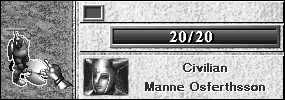
\includegraphics[width=0.4\textwidth]{Ipeasant2}
\end{center}
\vspace{-20pt}
\end{wrapfigure}

If you \textbf{Click} on any unit, you will be shown, as you can see on the right, more details on the unit.

\clearpage

\section{Map Modes}

\begin{center}
	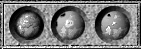
\includegraphics[width=0.4\linewidth]{Imapmode}
\end{center}

On the top left of your screen, you will see the three \textbf{World Map Mode Buttons}. These are, left to right: \textbf{Terrain View Button}, \textbf{Borders View Button}, and \textbf{Village View Button}.

\subsection{Terrain View Button}

\index{World Map modes!terrain view}

This is the default mode. When \textbf{Clicked}, it will show the World Map in relief and in its natural colors. You will also be able to see Villages, Troop, and Ship movements in the color of their respective Kingdoms.

\subsection{Borders View Button}

\index{World Map modes!border view}

The center button has two modes in itself. \textbf{Clicking} on it the first time will show the political borders of each kingdom on the World Map. You may also view all Troop and Ship movements. \textbf{Clicking} on this button a second time will project those political borders onto the main screen area.

Units of other Kingdoms will try to walk around your borders in their travels. This, of course, does not include Caravans or Soldiers who are coming to attack you.

\subsection{Village View Button}

\index{World Map modes!village view}

\textbf{Clicking} on this button will show you a simplified World Map with all Villages and all buildings clearly displayed. You may also view all Troop and Ship movements. Forested areas will not be shown on this map.

\section{Unit Information}

\begin{wrapfigure}{r}{0.5\textwidth}
	\vspace{-20pt}
	\begin{center}
		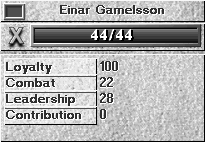
\includegraphics[width=0.4\textwidth]{Iunitinfo}
	\end{center}
	\vspace{-20pt}
\end{wrapfigure}

Whenever you \textbf{Click} on one of your units, you will be presented with information showing that unit’s Color, Name, Hit-Points, Loyalty Level, Combat Skill Level, Leadership Level, and Contribution Total.

Every person in the world of \textit{Seven Kingdoms: Ancient Adversaries} bears a unique name.

% CORRECT?

To center a selected Person, Weapon, Ship, Caravan, or Building on the main screen, \textbf{Click} on its name.

\section{News}

\index{news}

On the bottom of your main screen, you will receive news of happenings from around the world. From the in-game Options menu, you may decide if you want to receive all of the news or just the major happenings.

On the bottom right of your main screen, you will be able to see two small icons.

If you want to clear all of the news from the screen, \textbf{Click} on the 
\includegraphics[width=0.02\linewidth]{Bx} Icon or press the X key on your keyboard.

If you want to view the complete News Log, showing all of the previous news reports, \textbf{Click} on the 
\includegraphics[width=0.02\linewidth]{Bnews} Icon.

Some of the news reports will have a “Go To” Icon in front of them. If you wish to go to the location of the news story, \textbf{Click} on the 
\includegraphics[width=0.02\linewidth]{Bgoto} Icon.
%*
%* Seven Kingdoms: Ancient Adversaries
%*
%* Copyright 1997,1998 Enlight Software Ltd.
%* Copyright 2018 Timothy Rink
%*
%* This program is free software: you can redistribute it and/or modify
%* it under the terms of the GNU General Public License as published by
%* the Free Software Foundation, either version 2 of the License, or
%* (at your option) any later version.
%*
%* This program is distributed in the hope that it will be useful,
%* but WITHOUT ANY WARRANTY; without even the implied warranty of
%* MERCHANTABILITY or FITNESS FOR A PARTICULAR PURPOSE.  See the
%* GNU General Public License for more details.
%*
%* You should have received a copy of the GNU General Public License
%* along with this program.  If not, see <http://www.gnu.org/licenses/>.
%*
%*

\chapter{The Village}

\textbf{\textgoth{\Huge{C}}lick} on any one of the small houses in your first Village. When you do, you will see the Village Command Bar to the right of the main screen.

\begin{center}
    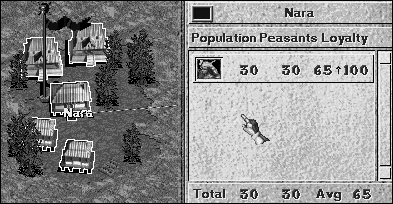
\includegraphics[width=0.9\linewidth]{Ivillage} % Original size.
\end{center}

\section{Village Demographics}

\index{demographics of village}
\index{villages!demographics}

\subsection{Population/Nationality}

\textgoth{\Huge{T}}he number on the lower left shows the total number of people in the selected Village. They are divided into their various national groupings, which you can distinguish by the small pictures on the far left. As long as you have not disabled the Help feature, holding your cursor over one of the small pictures for a few seconds will pop up a text bubble telling you which nationality it is.

Although there may be up to seven different nationalities in Villages that you will later build, absorb, or conquer, in your first Village there will be only one.

The style of houses in Villages will give you a quick idea as to what nationalities reside there.

To see what types of houses belong to which nationalities, see the house images in \textbf{Chapter 14}.

Populations in Villages will increase over time up to a maximum of 60. The rate of increase will not be the same for all Villages because Villages which have access to a steady supply of consumer goods will grow faster than those without. Higher standards of living induce higher growth rates.

See \textbf{Chapter 20} for Economic Strategy Tips.

\subsection{Peasants}

\index{peasants}

\textgoth{\Huge{A}}t the bottom of the middle column, you will see the total number of Peasants at work in the fields of this Village. They can either be left toiling in the fields, trained in various skills, ordered to work in other jobs, or sent out to be instructed in the ways of war.

Because Peasants grow all of the food for your empire, it is important to leave enough of them working in the fields. Each Peasant will produce 30 units of food per year, and each subject of your kingdom will consume 10 units per year. Thus, to maintain a sufficient food supply, you must have at least one Peasant for every three subjects.

\clearpage

\subsection{Loyalty}

\index{loyalty}

\begin{wrapfigure}{r}{0.4\textwidth}
    \vspace{-20pt}
    \begin{center}
        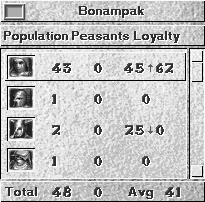
\includegraphics[width=0.4\textwidth]{Ivillage_peasants} % Original size.
    \end{center}
    \vspace{-20pt}
\end{wrapfigure}

These numbers (on the far right) show the level of Loyalty to your kingdom for each Nationality in a Village. The arrows indicate whether this Loyalty is increasing or decreasing.

On the bottom right, you can see the average Loyalty Level for all of the Nationalities in the Village.

If the Loyalty of a Nationality in one of your Villages falls to 30 or below, there will be a danger of revolt in that group.

% impacts? plural or singular verb?

Low Loyalty levels may also have negative impacts other than open revolt. Individual Villagers may leave your Villages for other Kingdoms, Independent Villages, or for unknown regions, although they will be most likely moved to a Village that is Linked to their present home.

\textbf{Loyalty Levels are positively influenced by:}

% Note this spot.

\begin{changemargin}{.5cm}{0cm}
Residential Harmony, which itself is a result of having a single Nationality in a Village rather than multiple Nationalities. The Villagers being of the same Nationality as the King.

A high Reputation for your Kingdom will help increase the Loyalty Level of all Villagers.

Having a General, in a Fort Linked to the Village, who is of the same Nationality as the Villagers. If the General has a high Leadership Level, the effect will be increased. If the General’s Nationality is the same as the King’s, the effect will be increased by an additional 50\%.
\end{changemargin}

\textbf{Loyalty Levels are negatively affected by:}

\begin{changemargin}{.5cm}{0cm}
Having a Fort from another Kingdom within Linking distance of your Village. If the rival General in that Fort is of the same Nationality as your Villagers, the effect will be increased, especially if he has a high Leadership Level.

A low Reputation for your Kingdom will hold down the Loyalty Level of all Villagers.
Recruiting Villagers or conscripting them directly into a Fort will lower a 

Village’s Loyalty somewhat for each Villager Recruited.
\end{changemargin}
    
\textbf{Loyalty Levels of Workers:}

\begin{changemargin}{.5cm}{0cm}
Since all Workers reside in Villages, their Loyalty Levels are reflected in the Loyalty Level of the Villages. This differs from Soldiers who reside inside Forts.
\end{changemargin}

\subsection{Quality of Life}

\index{quality of life}

\textgoth{\Huge{H}}aving a high Quality of Life in your Villages will cause their population to grow faster. With a large population, you will have an abundance of the most precious resource in \textit{Seven Kingdoms: Ancient Adversaries}, People.

Even the most ruthless of tyrants will benefit from improving his subjects’ lifestyle. If you wish your Villagers to have a high Quality of Life, you must make sure that they have access to consumer goods in Markets. The greater the quantity and variety of goods for them to buy, the higher their Quality of Life will be.

\section{Commanding Your Peasants}

\index{commanding peasants}

\subsection{Recruit}

\index{recruiting peasants}

\begin{wrapfigure}{r}{0.1\textwidth}
    \vspace{-20pt}
    \begin{center}
        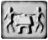
\includegraphics[width=0.1\textwidth]{Trecruit}
    \end{center}
    \vspace{-20pt}
\end{wrapfigure}

% Capitalization here.

\textgoth{\Huge{W}}ith this command, you order your peasants out of their Villages and assign them where you will. Have a care, though; Peasants resent this conscription, and there is therefore a small decrease in Village loyalty for each peasant recruited.

The rate of the decrease will depend upon the frequency of your Recruiting. Infrequent Recruiting will result in a lower Loyalty decrease than frequent Recruiting.

This tile will no longer be available if there are no more Peasants left in your Village.

\clearpage

\subsection{Moving between Villages}

\index{moving between villages}
\index{villages!moving between}

\begin{wrapfigure}{r}{0.6\textwidth}
    \vspace{-20pt}
    \begin{center}
        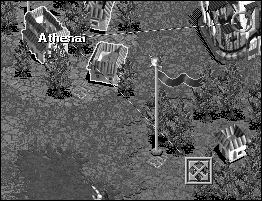
\includegraphics[width=0.6\textwidth]{Ivillage_villagelink} % Original size.
    \end{center}
    \vspace{-20pt}
\end{wrapfigure}

% Hyphenation here.

\textgoth{\Huge{I}}f you settle a new Village within Linking distance of an older Village, you will, when either of the Villages is selected, see a bright pink 4-Arrow Icon at the end of the Link.

% Hyphenation here.

If you wish to move Villagers from one Village to another \textbf{\textit{without}} suffering the decrease in Loyalty that you get when Recruiting Villagers, you may \textbf{Right-Click} on the Pink 4-Arrow Icon. One Villager at a time will then move from the selected Village into the Village under the Icon when \textbf{Left-Clicking}; when \textbf{Right-Clicking}, ten Villagers will moved.

\subsection{Train}

\index{training peasants}

\begin{wrapfigure}{r}{0.1\textwidth}
    \vspace{-20pt}
    \begin{center}
        
\includegraphics[width=0.1\textwidth]{Ttrain}
    \end{center}
    \vspace{-20pt}
\end{wrapfigure}

% Hyphenation here: Non-

\textgoth{\Huge{A}}ny Peasant may be trained in any of several useful skills. Training each unit will cost \$30. At the end of his training, which will take five days, the new Worker will have a skill level of 20. This skill will soon grow if he is put to work. Non-trained units who go to work will also see their skill levels increase, although from a starting level of 10.

Some workers are born with an inborn potential that outstrips that of their peers. Their Skill Levels will increase at a faster rate.

\subsubsection{How to Train a Unit}

\textgoth{\Huge{F}}irst select the Village where you want the Peasant to be trained in a new skill.

% Capitalization after colon here.

\textbf{NOTE:} If you have no Fort linked to the Village, or if you have a Fort that is not staffed with a General or King, this Tile will not be available, and you will be unable to train anyone.

Then \textbf{Click} on the \textbf{Train Tile} (above). The six Training Categories will appear on the right of your screen.

\textbf{Click} on the skill that you want, and one Peasant will begin training in his new profession.

\begin{wrapfigure}{r}{0.4\textwidth}
    \vspace{-20pt}
    \begin{center}
        
\includegraphics[width=0.4\textwidth]{Itrainprogress} % Original size.
    \end{center}
    \vspace{-15pt}
\end{wrapfigure}

% X is bold here.

You may cancel the training of a unit by \textbf{Clicking} on the large \textbf{X} to the right of the blue progress bar.

\subsubsection{How to Train more than one Unit at a time}

% Outdated image.

\begin{wrapfigure}{r}{0.35\textwidth}
    \vspace{-20pt}
    \begin{center}
        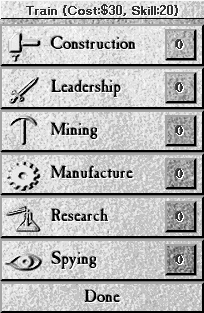
\includegraphics[width=0.35\textwidth]{Itrain} % Original size.
    \end{center}
    \vspace{-20pt}
\end{wrapfigure}

\textgoth{\Huge{T}}o the right of the Skill description, you will see another, smaller button with a number on it.

\textbf{Click} on this button repeatedly until it shows the number of Peasants that you want to train in a new skill.

\textbf{Right-Clicking} on the number button will decrease the number by one.

You may set numbers for more than one skill at a time.

When you are finished, \textbf{Click} on the \textbf{Done Button}. The Workers and/or Soldiers with their new skills will exit the Village one at a time as they are trained.

All Trained Units will begin with a Skill Level of 20.

% semicolon proper? Quotation marks here. informal. COMMA

Trained Units; Skill Levels will steadily increase, but only while they are at work. “At work” does not only mean being in their place of work; they must have something to do while there. For example, if a Factory has no Raw Materials to work with, then the skill of the workers will not increase.

\subsubsection{Construction}

\index{skills!construction}
\index{construction skill}

\begin{wrapfigure}{r}{0.1\textwidth}
    \vspace{-20pt}
    \begin{center}
        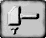
\includegraphics[width=0.1\textwidth]{Thammer}
    \end{center}
    \vspace{-20pt}
\end{wrapfigure}

% (see below): Bold?

\textgoth{\Huge{A}} unit trained in Construction is necessary to supervise the erection of most Buildings. Although other trained units (see below) may build certain structures, a unit trained in Construction will be able to build them all.

Construction of a Building will be suspended if the building is under attack.

In order to repair a damaged building, a worker trained in Construction must be assigned to it. To do this, send a selected Construction unit into any Building with a \textbf{Right-Click}.

The speed of a building’s construction or repairs will depend on the Skill Level of the Construction worker. The higher his skill, the faster he will build or repair.

\subsubsection{Leadership}

\index{skills!leadership}
\index{leadership skill}

\begin{wrapfigure}{r}{0.1\textwidth}
    \vspace{-20pt}
    \begin{center}
        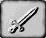
\includegraphics[width=0.1\textwidth]{Tleadership}
    \end{center}
    \vspace{-20pt}
\end{wrapfigure}

% Comma here

\textgoth{\Huge{A}} unit trained in Leadership serves as a soldier in your kingdom’s military, or be promoted to General. Upon completion of Leadership training, a unit will have an initial skill of 20 in both Leadership and Combat. If later promoted to Generals, trained leaders are also effective in helping your Empire to absorb independent Villages. Units trained in Leadership will be able to erect Forts, and having been used for this, they will immediately be assigned there when construction is complete.

\subsubsection{Mining}

\index{skills!mining}
\index{mining skill}

\begin{wrapfigure}{r}{0.1\textwidth}
    \vspace{-20pt}
    \begin{center}
        
\includegraphics[width=0.1\textwidth]{Tmining}
    \end{center}
    \vspace{-20pt}
\end{wrapfigure}

\textgoth{\Huge{A}} unit trained in Mining will begin as a more productive Miner, producing more raw materials for your factories than an untrained worker can. Units trained in Mining will also be able to dig Mines. If they are used for this, they will immediately be assigned there to begin their work.

\begin{wrapfigure}{r}{0.1\textwidth}
        \begin{center}
        
\includegraphics[width=0.1\textwidth]{Tmanufacturing}
    \end{center}
    \vspace{-20pt}
\end{wrapfigure}

\subsubsection{Manufacturing}

\index{skills!manufacturing}
\index{manufacturing skill}

\textgoth{\Huge{A}} unit trained in Manufacturing will begin working in your Factories and War Factories as a more productive worker than one who is untrained. Units trained in Manufacturing will be able to erect Factories and War Factories. If they are used for this, they will immediately be assigned there to begin production.

\begin{wrapfigure}{r}{0.1\textwidth}
        \begin{center}
        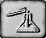
\includegraphics[width=0.1\textwidth]{Tresearch}
    \end{center}
    \vspace{-20pt}
\end{wrapfigure}

\subsubsection{Research}

\index{skills!research}
\index{research skill}

\textgoth{\Huge{A}} unit trained in Research will aid you in discovering the technologies needed to build Advanced Weapons and Ships.

Units trained in Research will be able to erect Towers of Science. If they are used for this, they will immediately be assigned there to begin their research.

\subsubsection{Spying}

\index{skills!spying}
\index{spying skill}

\begin{wrapfigure}{r}{0.1\textwidth}
    \vspace{-20pt}
    \begin{center}
        
\includegraphics[width=0.1\textwidth]{Tspy}
    \end{center}
    \vspace{-20pt}
\end{wrapfigure}

\textgoth{\Huge{A}} unit trained in Spying will be able to penetrate enemy Villages, influencing the Villagers’ loyalty, and give you all the information on the population that your enemy himself possesses. Spies may penetrate firms, quietly sabotaging production.

% FACTUAL?

Drinking in enemy Inns, they may be recruited and put into an important position in their society. They may even penetrate enemy Forts, giving you unrivaled intelligence on Combat levels, and giving your Spy the opportunity to assassinate a General or a King. 

For many more details on Spies and Espionage, see \textbf{Chapter 13}.

\subsubsection{More Details on all Trained Units}

\textgoth{\Huge{W}}hen outside and selected, all of your trained units will show a small icon above their heads denoting their particular specialty. These icons are the same as those appearing on the Train menu.

When you place your cursor over subjects of another kingdom, you will also be able to see their particular skill.

Any enemy unit without a Sword Icon is a civilian. It is good to know this as it will hurt your Kingdom’s Reputation if you attack civilians.

% Therefore here. Hypehnation is lacking here.

You should realize that your King and your Generals are easily recognizable to both friends and foes. It is therefore imperative that you protect these valuable units as best you can, because in battle, both human and computer controlled foes will probably attempt to slay your commanders first.

The productivity levels of all trained workers who have been injured will decline in proportion to their injury. Injury will also slow down the speed of their training.

% COMMA HERE

The same rule applies to training soldiers. If a fort’s commander is injured, the training of his Troop will be slowed, as will any increase to his own Leadership skill.

When a unit is sent to work in a building that already has a full complement of workers, he will replace the worker with the lowest skill level. That replaced worker will return to a Linked Village where he will live as a Peasant.

If you send a soldier into an already full Fort, one soldier from the Fort will then exit and stand outside. He will not Settle in a Village.

\begin{wrapfigure}{r}{0.5\textwidth}
    \vspace{-20pt}
    \begin{center}
        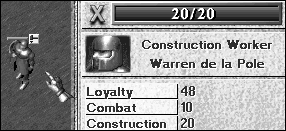
\includegraphics[width=0.5\textwidth]{Ipeasant} % Original size.
    \end{center}
    \vspace{-20pt}
\end{wrapfigure}

You may easily view the identity and other pertinent information on any unit by selecting it. The unit’s information will be displayed on the right. \\ % adds vspace due to wrapfig.

\section{Collect Tax}

\index{collecting taxes}
\index{taxes}

\textgoth{\Huge{T}}axes are yours to command from your people. In \textit{Seven Kingdoms: Ancient Adversaries}, there are two types of taxes. The Yearly Tax will be collected every January 1st from every person living in your Villages.

\begin{wrapfigure}{r}{0.1\textwidth}
    \vspace{-20pt}
    \begin{center}
        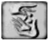
\includegraphics[width=0.1\textwidth]{Ttax}
    \end{center}
    \vspace{-20pt}
\end{wrapfigure}

Special Taxes may also be collected from each person living in a selected Village. When a Special Tax is collected, the Loyalty Level of all Villagers in the selected Village will decrease. The amount of the decrease will depend upon how often your tax collectors come calling. Collecting Taxes several times in quick succession will result in far greater loss of Loyalty than taxing over a greater period of time.

There will be no decrease in loyalty for the Yearly Tax.

\clearpage

% Outdated graphic.

\begin{wrapfigure}{r}{0.3\textwidth}
    \vspace{-20pt}
    \begin{center}
        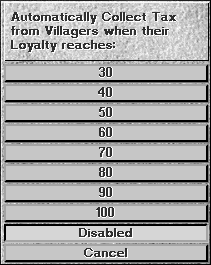
\includegraphics[width=0.3\textwidth]{Iautotax} % Original size.
    \end{center}
    \vspace{-20pt}
\end{wrapfigure}

\textbf{Auto-Taxing a Single Village}: If you \textbf{Right-Click} on the \textbf{Tax Tile}, you will be presented with a list of Loyalty Levels. By \textbf{Clicking} on one of these, you will automatically collect a Special Tax from the selected Village whenever their Loyalty reaches this level.

\textbf{Auto-Taxing All Villages}: By \textbf{Right-Clicking} on one of the numbers, instead of \textbf{Clicking}, you will, in the future, collect a Special Tax from every one of your Villages when their average Loyalty Level reaches the selected level.

This will also apply to new Villages when they are settled.

\subsection{Grant}

\index{grants}

\begin{wrapfigure}{r}{0.1\textwidth}
    \vspace{-20pt}
    \begin{center}
        
\includegraphics[width=0.1\textwidth]{Tgrant}
    \end{center}
    \vspace{-20pt}
\end{wrapfigure}

\textgoth{\Huge{G}}rants are the exact opposite of taxes. If you find some of your Villages’ Loyalty lacking, common peasants and workers are easily placated by spreading a little of your excess treasure around. Assuming that you have abundant funds, providing Grants to Villages around your Empire to ensure complete loyalty makes very good sense.

Each Grant will distribute \$10 to every Villager in the selected Village. The Villagers will then show an increase in their Loyalty Levels. The amount of increase will vary depending upon how often you Grant money to them. Issuing several Grants in rapid succession will have less effect than spreading your generosity out over a greater span of time.

% COMMA HERE

Grants may also be issued to Independent Villages if you have a Fort Linked to them and staffed with a General or your King. Each Grant to an Independent Village will cost you \$30 per Villager. These Grants will quickly lower the resistance of that Village to your rule, but at great cost to you.

You may also Grant money to Villagers of other Kingdoms if you have a staffed Fort Linked to their Village, and the other kingdom does not. These Grants will lower the Loyalty Level of those Villagers to their King.

\clearpage

% Outdated graphic.

\begin{wrapfigure}{r}{0.3\textwidth}
    \vspace{-20pt}
    \begin{center}
        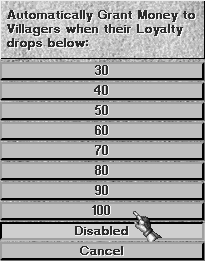
\includegraphics[width=0.3\textwidth]{Iautogrant} % Original size.
    \end{center}
    \vspace{-20pt}
\end{wrapfigure}

\textbf{Auto-Granting to a Single Village}: You may automatically Grant funds to your selected Village by first \textbf{Right-Clicking} on the \textbf{Grant Tile} and then \textbf{Clicking} on the Loyalty Level at which you wish to make your Grants.

\textbf{Auto-Granting to All Villages}: By \textbf{Right-Clicking} on one of the numbers, you will automatically Grant money to every one of your Villages when their average Loyalty Level drops to the selected level.

\begin{wrapfigure}{r}{0.1\textwidth}
    \vspace{-20pt}
    \begin{center}
        
\includegraphics[width=0.1\textwidth]{Tautotax100}
    \end{center}
    \vspace{-20pt}
\end{wrapfigure}

When you have set Auto Tax or Auto Grant, the level to which you have set it will be displayed on top of the \textbf{Tax} or \textbf{Grant Tiles}. \\

\begin{wrapfigure}{r}{0.1\textwidth}
    \vspace{-20pt}
    \begin{center}
        \includegraphics[width=0.1\textwidth]{Tautogrant40}
    \end{center}
    \vspace{-20pt}
\end{wrapfigure}

\textbf{NOTE}: The Auto Tax Loyalty Level must always be set higher than the Auto Grant Loyalty Level. If you do not set it so, the computer will automatically set it to be 10 points higher.

%*
%* Seven Kingdoms: Ancient Adversaries
%*
%* Copyright 1997,1998 Enlight Software Ltd.
%* Copyright 2018 Timothy Rink
%*
%* This program is free software: you can redistribute it and/or modify
%* it under the terms of the GNU General Public License as published by
%* the Free Software Foundation, either version 2 of the License, or
%* (at your option) any later version.
%*
%* This program is distributed in the hope that it will be useful,
%* but WITHOUT ANY WARRANTY; without even the implied warranty of
%* MERCHANTABILITY or FITNESS FOR A PARTICULAR PURPOSE.  See the
%* GNU General Public License for more details.
%*
%* You should have received a copy of the GNU General Public License
%* along with this program.  If not, see <http://www.gnu.org/licenses/>.
%*
%*

\chapter[Buildings, Workers, \& Links]{{\Huge B}UILDINGS, {\Huge W}ORKERS, {\Huge \&} {\Huge L}INKS}

\section{Constructing Your Buildings}

\index{buildings!constructing}
\index{constructing buildings}

\begin{wrapfigure}{r}{0.1\textwidth}
    \vspace{-20pt}
    \begin{center}
        \includegraphics[width=0.1\textwidth]{Thammer}
    \end{center}
    \vspace{-20pt}
\end{wrapfigure}

\textswab{\huge{A}} unit trained in Construction is necessary to supervise the erection of most Buildings. Although other trained units may erect certain structures, a unit trained in Construction will be able to erect them all.

To construct a Building, first select the unit that will do the construction and then \textbf{Click} on the \textbf{Build Tile}.

You will be presented with a list of structures that the unit has the ability to construct. When you \textbf{Click} on the one that you want, your cursor will change into a large black or flashing box.

\begin{wrapfigure}{r}{0.45\textwidth}
    \vspace{-20pt}
    \begin{center}
        \includegraphics[width=0.45\textwidth]{Ibuildbox} % Original size.
    \end{center}
    \vspace{-20pt}
\end{wrapfigure}

The box will be black if it is over an area where you may not build. It will be flashing if it is over an acceptable area.

\textbf{Click} when the box is flashing and in the area where you want to build. Note that mines must be built atop Natural Resource deposits. 

Construction of a Building will be suspended if the building is under attack.

The speed of a building’s construction will depend on the Skill Level of the Construction worker. The higher his level, the faster the construction.

Construction workers will increase their skill whenever they are engaged in construction or repair.

If you use a Construction worker to put up a structure, he will exit the building when his work is finished. If you use a Manufacturer to build a Factory, a Miner to build a Mine, a Researcher to build a Tower of Science, or a Soldier to build a Fort, he will remain inside the building when construction has been completed.

\section{Selling Your Buildings}

\index{buildings!selling}
\index{selling buildings}

\begin{wrapfigure}{r}{0.4\textwidth}
    \vspace{-20pt}
    \begin{center}
        \includegraphics[width=0.4\textwidth]{Ifullheath_building}
    \end{center}
    \vspace{-20pt}
\end{wrapfigure}

\textswab{\huge{Y}}ou will be able to Sell your building by \textbf{Clicking} on the \$ Icon. This icon will only be visible when your structure is no more than 20\% damaged.

For the sale of an undamaged building, you will receive 50\% of the original cost of the building. If it is damaged, you will receive somewhat less, depending on the extent of the damage. You may also sell your building before you have finished its construction.

\section{Demolishing Your Buildings}

\index{buildings!demolishing}
\index{demolishing buildings}
    
\begin{wrapfigure}{r}{0.4\textwidth}
    \vspace{-20pt}
    \begin{center}
        \includegraphics[width=0.4\textwidth]{Idamage}
    \end{center}
    \vspace{-20pt}
\end{wrapfigure}

\textswab{\huge{I}}f your building is more than 20\% damaged, you will no longer have the option of selling it. You may either demolish it or repair it. You may demolish a building by \textbf{Clicking} on the Wrecking Ball Icon.

You will recoup no money when you demolish a building. You may also demolish your building before you have finished its construction.

% resident?

When buildings, except for Forts and Seats of Power, are demolished or sold, the workers in them will return to their Village and lose all skills that they have acquired. If there is a Construction worker in the building, he will remain a Construction worker and will be seen standing on the site of the old building. If a Fort or a Seat of Power is demolished or sold, those resident at the time will be seen standing on the site of their old building.

\section{Repairing Your Buildings}

\index{buildings!repairing}
\index{repairing buildings}
    
\begin{wrapfigure}{r}{0.4\textwidth}
    \vspace{-20pt}
    \begin{center}
        \includegraphics[width=0.4\textwidth]{Irepair_building}
    \end{center}
    \vspace{-10pt} % -10pt
\end{wrapfigure}

\textswab{\huge{A}} building may be repaired by sending a Construction unit into it. This Construction unit will not take the place of any other worker or soldier. While he is in the building, his Hammer Icon will appear next to the Sell or Demolish Icon.

Your Construction Worker will constantly repair your building, except when it is under attack. While repairing a building, he will also be increasing his skill in construction.

If you wish to take the Construction Worker out of the building, \textbf{Click} or \textbf{Right-Click} on the Hammer Icon.

\section{Units in Buildings}

\index{buildings!units inside}
\index{units!inside buildings}

\begin{wrapfigure}{r}{0.4\textwidth}
    \vspace{-20pt}
    \begin{center}
        \includegraphics[width=0.4\textwidth]{Ifullfort} % Original size.
    \end{center}
    \vspace{-10pt}
\end{wrapfigure}

\textswab{\huge{W}}henever you \textbf{Click} on one of your Buildings, you will be able to see its state of repair, its color and name, all of the People currently inside and the health and status of each of them.

To see information on an individual unit inside the building, \textbf{Click} on its picture. The unit will then be highlighted in yellow, and its information will be shown below.

\subsection{Mobilizing/Laying off Working Units}

\index{units!laying off}
\index{units!mobilizing}

\textswab{\huge{T}}o take a worker out of his building for reassignment elsewhere, first \textbf{Click} on the building where he is working. Next, \textbf{Click} on his icon on the command bar to the right of the screen. With the unit’s icon highlighted in yellow, \textbf{Right-Click} on it. He will then exit the building with all of his skills intact.

If you wish to lay off a worker and send him back to his Village, first select his place of work and then close the Link between it and the Village. Do this by \textbf{Clicking} inside the rotating green and yellow ring centered over the Village. With this Link closed, nobody from the Village will be able to come to work in that building. This is a good way to control your number of workers.

Now select the worker by \textbf{Clicking} on his picture. He should then be highlighted in yellow. Send him back to his Village by \textbf{Right-Clicking} on the green cross (closed Link).

\begin{wrapfigure}{r}{0.4\textwidth}
	\vspace{-20pt}
	\begin{center}
		\includegraphics[width=0.4\textwidth]{Icloselink} % Original size?
	\end{center}
	\vspace{-10pt}
\end{wrapfigure}

You may do this in exactly the same way for your people who are working in the firms of other Kingdoms. If, in the future, you wish to hire some more workers from that Village, you will have to \textbf{Click} again on the green X, thus opening up the Link.

\subsection{Changing a Worker’s Residence}

\index{changing a unit's residence}
\index{units!changing residence}

\begin{center}
    \includegraphics[width=0.6\linewidth]{Iresidencechange} % Original size.
\end{center}

\textswab{\huge{I}}f you wish to move a Worker from one Village to another, you must first \textbf{Click} on his place of work and then on his picture. If that place of work is Linked to more than one Village, you will then be able to move his residence.

His present Village is the one that has the double-Link line between it and his place of work. To move his residence to another Village, \textbf{Right-Click} inside the rotating ring centered on that other Village.

\section{Linking Your Buildings}

\index{buildings!linking}
\index{linking buildings}

\textswab{\huge{L}}inks are established when buildings are built within a certain distance of one another. You can tell if buildings or Villages are linked when there is a Linking Line connecting them.

\subsection{Open Links}

\index{open links}
\index{links!open}

\begin{wrapfigure}{r}{0.5\textwidth}
    \vspace{-20pt}
    \begin{center}
        \includegraphics[width=0.5\textwidth]{Iopenlink_fort} % Original size.
    \end{center}
    \vspace{-20pt}
\end{wrapfigure}

\textswab{\huge{L}}inks are open and functioning when the yellow and green ring at the end of a line is rotating. An open Link means that goods, money, people, and influence can flow between both ends of the line.

\subsection{Closed Links}

\index{closed links}
\index{links!closed}

\begin{wrapfigure}{r}{0.3\textwidth}
    \vspace{-20pt}
    \begin{center}
        \includegraphics[width=0.3\textwidth]{Icloselink_fort} % Original size.
    \end{center}
    \vspace{-10pt}
\end{wrapfigure}

\textswab{\huge{Y}}ou may close an open Link by \textbf{Clicking} inside the rotating yellow and green ring. The ring will then change to a green X.

All flow between the two ends of the Link will then cease. This is useful for controlling the number of workers who can volunteer to work in your structures as well as for controlling the flow of goods and raw materials.

\section{Inactive Links}

\index{inactive links}
\index{links!inactive}

\begin{wrapfigure}{r}{0.5\textwidth}
    \vspace{-20pt}
    \begin{center}
        \includegraphics[width=0.3\textwidth]{Iinactivelink}
    \end{center}
    \vspace{-50pt}
\end{wrapfigure}

\textswab{\huge{L}}inks are inactive when the rings on the end of them are a solid orange in color. Inactive Links cannot be rendered active by you. They are controlled by Independent Villages or by other Kingdoms. 

\subsection{Fort-Village Links}

\index{fort-village links}
\index{links!fort-village}

\textswab{\huge{A}}n open Link between a Fort and a Village will allow the King or General in the Fort to exert their authority over the Village.

\begin{wrapfigure}{r}{0.5\textwidth}
    \vspace{-20pt}
    \begin{center}
        \includegraphics[width=0.7\textwidth]{Iactivelink_fort}
    \end{center}
    \vspace{-50pt}
\end{wrapfigure}

\subsection{Village-Firm Links}

\index{links!village-firm}
\index{village-firm links}

\begin{center}
    \includegraphics[width=1\linewidth]{Imultilinks} % Original size.
\end{center}

\textswab{\huge{A}}n open Link between a Village and a Firm (any building that employs workers) will allow Peasants from the Village to volunteer to work in the Firm.

Up to eight Peasants may volunteer to fill the open working slots in each firm.

If a Firm is built outside of Linking distance to a Village, you must remember to Recruit Peasants and send them to work there. There is no way for the Peasants to volunteer.

\subsection{Village-Market Links}

\index{links!village-market}
\index{village-market links}

\begin{wrapfigure}{r}{0.5\textwidth}
    \vspace{-20pt}
    \begin{center}
        \includegraphics[width=0.5\textwidth]{Ilink_villagemarket} % Original size.
    \end{center}
    \vspace{-20pt}
\end{wrapfigure}

\textswab{\huge{A}}n open Link between a Village and a Market will allow residents of the Village to buy goods from the Market.

It is a good idea, if possible, to build a Market within Linking distance of more than one Village.

Links between your Markets and your Villages will always be open. You may not close them.

Links between Villages and Foreign Markets will be open or closed depending on whether or not the two Kingdoms have a trade treaty. You will be unable to open or close the Link manually.

\subsection{Market-Factory Links}

\index{links!market-factory}
\index{market-factory links}

\begin{wrapfigure}{r}{0.2\textwidth}
    \vspace{-20pt}
    \begin{center}
        \includegraphics[width=0.2\textwidth]{Ilink_factorymarket} % Original size.
    \end{center}
    \vspace{-20pt}
\end{wrapfigure}

\textswab{\huge{A}}n open Link between a Market and a Factory will allow the Finished Goods from the Factory to be immediately sent to the Market for sale.

This will be the most efficient arrangement because it eliminates the need for a Caravan Link.

\clearpage

\subsection{Market-Mine Links}

\index{links!market-mine}
\index{market-mine links}

\begin{wrapfigure}{r}{0.5\textwidth}
    \vspace{-20pt}
    \begin{center}
        \includegraphics[width=0.5\textwidth]{Ilink_marketmine} % Original size.
    \end{center}
    \vspace{-10pt}
\end{wrapfigure}

\textswab{\huge{A}}n open Link between a Market and a Mine will allow the mined Raw Materials from the Mine to be placed in the Market for sale, either to one of your Factories that is Linked to the Market or to any Caravans that call at the Market.

This arrangement is most often used when you wish to sell Raw Materials to other Kingdoms, as their Caravans will be able to call at your Markets and not at your Mines.

\subsection{Factory-Mine Links}

\index{factory-mine links}
\index{links!factory-mine}

\begin{wrapfigure}{r}{0.4\textwidth}
    \vspace{-20pt}
    \begin{center}
        \includegraphics[width=0.4\textwidth]{Ilink_minefactory} % Original size.
    \end{center}
    \vspace{-20pt}
\end{wrapfigure}

\textswab{\huge{A}}n open Link between a Factory and a Mine will enable the Factory to receive immediate delivery of the Raw Materials that it needs to produce Finished Goods.

This arrangement is the most efficient because it eliminates the need for a Caravan to carry Raw Materials to the Factory.

\clearpage

\subsection{Market, Factory, and Mine-Harbor Links}

\index{links!market, factory, mine-harbor}
\index{market, factory, mine-harbor links}

\begin{center}
    \includegraphics[width=0.95\linewidth]{Ilink_harbor} % Original size.
\end{center}

\textswab{\huge{A}}n open Link between a Market, Factory or Mine and a Harbor enable Ships calling at the Harbor to pick up either Finished Goods or Raw Materials from those places.

Your Ships will also be able to drop off their cargo from foreign lands. These goods will be immediately transferred to the Market.

The Link between your Village and your Harbor will always be open. You will not be able to close it.

A Link between your Market and a Foreign Harbor will be open or closed depending on whether or not you have a trade treaty with that Foreign Kingdom. You will be unable to open or close the Link manually.
%*
%* Seven Kingdoms: Ancient Adversaries
%*
%* Copyright 1997,1998 Enlight Software Ltd.
%* Copyright 2018 Timothy Rink
%*
%* This program is free software: you can redistribute it and/or modify
%* it under the terms of the GNU General Public License as published by
%* the Free Software Foundation, either version 2 of the License, or
%* (at your option) any later version.
%*
%* This program is distributed in the hope that it will be useful,
%* but WITHOUT ANY WARRANTY; without even the implied warranty of
%* MERCHANTABILITY or FITNESS FOR A PARTICULAR PURPOSE.  See the
%* GNU General Public License for more details.
%*
%* You should have received a copy of the GNU General Public License
%* along with this program.  If not, see <http://www.gnu.org/licenses/>.
%*
%*

\chapter[Force and Its Use]{\textsf{FORCE AND ITS USE}}

\index{using force} % expand?

\section{\textsf{The Fort}}

\begin{wrapfigure}{l}{0.3\textwidth}
    \vspace{-20pt}
    \begin{center}
        \includegraphics[width=0.3\textwidth]{Ifort}
        \\ Fort
    \end{center}
    \vspace{-30pt} % -30pt
    \end{wrapfigure}

\textswab{\huge{Y}}our first Fort will be immediately visible when you begin a new game. \textbf{Click} on this Fort, and you will see its only resident: your King. In order to issue commands to your Villagers, you must have a linked Fort staffed by either your King or a General. As your King has the highest level of leadership in your Empire and is already stationed there, there is no need to train any other leaders just yet.

\subsection{\textsf{Conscription and Training}}

\index{conscription}

\textswab{\huge{I}}n order to fill up your Fort and train Soldiers, you must conscript Peasants into your armed forces.

\subsubsection{\textsf{How do you conscript Peasants?}}

\begin{wrapfigure}{r}{0.1\textwidth}
    \vspace{-20pt}
    \begin{center}
        \includegraphics[width=0.1\textwidth]{Trecruit}
    \end{center}
    \vspace{-20pt}
\end{wrapfigure}

First \textbf{Click} on the Village whose Peasants you wish to conscript and then \textbf{Click} on the \textbf{Recruit Tile} once for each Peasant that you wish to conscript. You may recruit up to eight Peasants for each Fort.

After eight or fewer Peasants have been recruited and are standing outside your Village, \textbf{Group Select} them and then order them into the Fort with a \textbf{Right-Click} on the Fort.

An alternative method of conscription is to select the Village and then to \textbf{Right-Click} inside the rotating ring centered on the Linked Fort. For every \textbf{Right-Click}, one peasant will be transferred into the Fort to begin his training.

Soldiers who have been assigned to a Fort will no longer live in the Village. The Fort will become their new residence.

Because only Villagers pay taxes, having a large percentage of your subjects in the army will severely restrict your tax base.

\subsubsection{\textsf{Combat and Leadership Levels}}

\index{combat and leadership levels}

\textswab{\huge{C}}onscripted Soldiers will start off with a Combat Level and a Leadership Level of just 10. While they are training in their Fort or while they are fighting, their Combat Level will increase. The speed of the increase depends on the Leadership Level of the General or King. If the commander’s Leadership Level is high, the soldier’s Combat Level will increase faster than if the commander’s Leadership Level were low.

The maximum combat level of any Soldier is 100.

A General’s or a new King’s Leadership will increase when training soldiers in a Fort or when soldiers under his command and within 10 spaces of him are engaged in battle.

A soldier’s Combat Level will never increase beyond the Leadership Level of his commander.

Generals or Kings will gain an improvement to their Leadership Level only if they have soldiers and/or Weapons to command. The more units they have under their command, the faster their Leadership ability will increase.

In a small percentage of your common soldiers, you may see a slow and steady increase in Leadership Level. These units should be watched and cultivated; they have an innate talent for Leadership and may make excellent Generals one day.

Training units who have been wounded and then returned to the Fort will be slower than training units that are completely well. This applies to both Combat Level and Leadership Level.

An injured General will also improve his Leadership Level more slowly than an uninjured one.

On the field of battle, a General’s Leadership Level is of critical importance. A General or King imparts a combat bonus to members of his own Troop equal to his Leadership Level. For example, if a General has a Leadership Level of 100, a Soldier or Weapon in his Troop will receive a 100\% bonus to his combat ability. This assumes that the General (or King) is no more than 10 spaces away from each Soldier or Weapon. Keeping your Generals safely away from battle is therefore not a good idea.

Units who are not part of a General’s troop receive no combat bonus while fighting within 10 spaces of him.

\subsubsection{\textsf{Hit-Point Bars}}

\index{hit-points bars}

\textswab{\huge{A}}bove the head of each selected unit, you will see a colored bar. There are three different colors that denote the maximum Hit-Points for any given unit.

A \textbf{Green} bar shows that the unit has a maximum of \textbf{between 20 and 50 Hit-Points}.

A \textbf{Yellow} bar shows that the unit has a maximum of \textbf{between 51 and 100 Hit-Points}.

A \textbf{Purple} bar shows that the unit has a maximum of \textbf{between 100 and the ultimate of 200 Hit-Points}.

\textbf{NOTE}: Although a unit may have only 5 Hit-Points remaining, only the length of the bar will change. The color will remain the same.

% Condenced sentences here.

A unit’s possible Hit-Point plateau will be twice his present Combat Skill Level. By paying attention to these colors, it will be to see where your most valuable units are and those of your rivals.

All units will recover their Hit Points at the fastest rate when they are safe inside a building. They will also recover at a slower rate while they are outside but not moving. If they are on the move, they will not recover.

\subsection{\textsf{Unit Alertness Modes in Forts}}

\index{altertness mode!in fort}
\index{units!alterness modes in forts}

\textswab{\huge{Y}}ou will have two options for the readiness of your troops inside their Fort: They may be ordered into either \textbf{Alert Mode} or \textbf{Stand Down Mode}.

\begin{wrapfigure}{r}{0.1\textwidth}
    \vspace{-20pt}
    \begin{center}
        \includegraphics[width=0.1\textwidth]{Talert}
    \end{center}
    \vspace{-20pt}
\end{wrapfigure}

When in \textbf{Alert Mode}, your Troops and Weapons inside a Fort will immediately Sortie to fight any foe who is attacking either their Fort or anything Linked to it. If that foe is defeated, your troops will then return to their Fort.

In this situation, your General will remain behind in the Fort directing operations. His leadership abilities will still influence his Troop and the Village to which the Fort is Linked.

\begin{wrapfigure}{r}{0.1\textwidth}
    \vspace{-20pt}
    \begin{center}
        \includegraphics[width=0.1\textwidth]{Tstanddown}
    \end{center}
    \vspace{-20pt}
\end{wrapfigure}

When in \textbf{Stand Down Mode}, your troops and weapons will stay safely behind the walls of your Fort until ordered otherwise. This may be a good idea if you are outnumbered and waiting for reinforcements.

\subsection{\textsf{Unit Alertness Modes outside of Forts}}

\index{altertness mode!outside fort}
\index{units!alterness modes outside forts}

\textswab{\huge{O}}utside of the Fort, troops in \textbf{Alert Mode} will behave with the intelligence that you would expect from real soldiers. They will automatically attack nearby enemy troops, (not civilians), but will not chase them out of the area unless so ordered by you. When attacking a structure, they will break off to defend themselves against an enemy attack. If they defeat that attack, they will return their attention to the targeted structure.

If troops come under attack while they are on their way to an assigned destination, they will stop and fight the enemy. Then, if they are victorious, they will continue their journey.

Troops outside their Fort in \textbf{Stand Down Mode} will more blindly follow orders. When an enemy approaches, they will not attack unless they are attacked first. When marching to another location, they will not stop to fight even when attacked, but will press on to their destination. They will only fight, in this case, if they are surrounded.

\subsection{\textsf{Sortie}}

\index{sortie}

\begin{wrapfigure}{r}{0.1\textwidth}
    \vspace{-20pt}
    \begin{center}
        \includegraphics[width=0.1\textwidth]{Tsortie}
    \end{center}
    \vspace{-20pt}
\end{wrapfigure}

\textswab{\huge{W}}hen your Fort is selected, \textbf{Click} on the \textbf{Sortie Tile}. The entire strength of your Fort will then sally forth to do your bidding. They will exit the Fort as a single Troop, selected and ready to do battle.

To select the group again later, \textbf{Right-Click} on any of the Soldiers in the Troop. The entire Troop will then be selected and awaiting your orders.

When a Troop is selected, you may order an attack on enemy Soldiers or on an enemy structure by \textbf{Right-Clicking} on the target. You will know that it is a valid target when your cursor turns red.

\subsection{\textsf{Numbering Groups}}

\index{numbering groups}

\textswab{\huge{Y}}ou may, if you wish, assign a number to a Troop, several Troops, or any group of people, Weapons, and/or Ships.

To do this, first \textbf{Select} or \textbf{Group-Select} the units that you want to number. Then press \textbf{Ctrl} + \textbf{number 0-9}. To recall a numbered group, press \textbf{Alt} + \textbf{number 0-9}.

Troops in a numbered group will lose their number if they return to their Fort. You may not, therefore, recall a numbered troop from its Fort.

Remember that when a Troop is sortied from its Fort, it is already grouped as a single unit that can be easily selected by \textbf{Right-Clicking} on any of its members.

If you have numbered a group of two or more Troops, you will still be able to select the individual Troops from within that group by \textbf{Right-Clicking} on any member. The selected Troop will still retain its assignment as a member of the numbered group if you wish to make use of it later.

\subsection{\textsf{Selecting Units in a Crowd}}

\index{selecting unit from a crowd}
\index{units!selecting from a crowd}

\textswab{\huge{S}}electing a single unit from within a crowd, or during a massive battle, can sometimes be difficult. To make it easier, hold down your \textbf{Ctrl key} while you \textbf{Click} on the area of the ground where the unit’s feet should be. The unit should then be selected. This selection method will work for all types of units.

\subsection{\textsf{Withdrawal}}

\index{units!withdrawal}

\begin{wrapfigure}{r}{0.1\textwidth}
    \vspace{-20pt}
    \begin{center}
        \includegraphics[width=0.1\textwidth]{Twithdrawl}
    \end{center}
    \vspace{-20pt}
\end{wrapfigure}

\textswab{\huge{T}}o return a selected Troop to its Fort, \textbf{Click} on the \textbf{Withdrawal Tile}. The Troop will immediately cease all present activity and march back to its Fort.

Even if your Troop is still being attacked, it will cease all fighting. In this case, the \textbf{Withdrawal Tile} will act as a quick retreat order. If members of a troop are surrounded by enemies and therefore cannot disengage from battle, they will continue fighting.

If you wish to send any selected units to another location without them stopping for \textbf{\textit{any}} reason, \textbf{Double-Click} on their destination.

\subsection{\textsf{Transfer}}

\index{transferring unit}
\index{units!transfer}

\textswab{\huge{T}}o transfer a soldier or soldiers from one Troop to another, \textbf{Click} on or Group Select them and then send them into another Fort with a \textbf{Right-Click}. They will then become members of that Fort’s Troop.

\subsection{\textsf{Waypoints}}

\index{setting!waypoints}
\index{units!setting wayspoints}

\textswab{\huge{T}}o set waypoints for your People, Ships, or Weapons to follow, first select the unit(s). Then, holding down the \textbf{Alt} key, \textbf{Right-Click} on either the world map or your main screen. For each \textbf{Right-Click}, you will set a waypoint. To set the last point, \textbf{Right-Click} without holding down the Alt key. Your selected units will begin to move as soon as the first waypoint has been set.

You may delete a waypoint (apart from the first) by \textbf{Right-Clicking} on the waypoint marker while the unit is selected.

Waypoints may \textbf{not} be used for Caravans or for Ships that are on trading routes.

\subsection{\textsf{The Death of a King}}

\index{death of king}
\index{king!death of}

\textswab{\huge{I}}f your King has been slain in battle, you must immediately choose a successor to the Crown. The longer you wait, the more restless and rebellious your people will become.

\begin{wrapfigure}{r}{0.1\textwidth}
    \vspace{-20pt}
    \begin{center}
        \includegraphics[width=0.1\textwidth]{Tcrown}
    \end{center}
    \vspace{-20pt}
\end{wrapfigure}

After the death of a King, upon selecting any unit, you will see the \textbf{Crown Tile} in the unit command bar. \textbf{Click} on this Tile if you want the selected unit to succeed to the Crown.

It is very important to your Empire that you select a unit with a high Leadership Level, because if the new King’s Leadership Level is less than the old King’s, your people’s loyalty will drop.

Also bear in mind the nationality of the majority of your population. Selecting a King from within this nationality may be the most prudent decision as the loyalty of people of Nationalities different from the new King will decrease.

Any other skills not befitting the station of a king, such as Spying, will be forgotten by a newly coronated unit. Combat and Leadership skills are retained.

\subsection{\textsf{Restoring Unit Health}}

\index{restoring unit health}
\index{units!restoring health}

\textswab{\huge{A}}ll Soldiers who have been wounded will eventually regain their full strength if they are not moved. If they are returned to a Fort, they will heal twice as fast.

\subsection{\textsf{Weapons in Forts}}

\index{weapons!in forts}

\textswab{\huge{Y}}ou may assign up to eight Weapons to a Fort, just as you would assign Soldiers. And just as with Soldiers, assigning a Weapon to a Fort commanded by a General makes the Weapon a part of that General’s Troop. When fighting within 10 spaces of the General, the Weapon and all other members of the Troop will receive a combat bonus equal to the General’s Leadership.

Your Weapons will be repaired in the Fort twice as fast as outside.

\subsection{\textsf{Promotion, or How to Make a General}}

\index{promoting units}
\index{units!promoting}

\textswab{\huge{E}}ach Fort, apart from the one that the King commands, needs a General to train the troops. A General is created by promoting a unit already trained in Leadership; that is one who has been trained either directly from one of your Villages or one who has learned soldiering skills as a common Soldier in his Fort.

\subsubsection{\textsf{How Do You Promote a Soldier?}}

\begin{wrapfigure}{r}{0.1\textwidth}
    \vspace{-20pt}
    \begin{center}
        \includegraphics[width=0.1\textwidth]{Tstar}
    \end{center}
    \vspace{-20pt}
\end{wrapfigure}

To promote a Soldier (with a small Sword Icon over his head) who is outside of a Fort, \textbf{Click} on him and then \textbf{Click} on the \textbf{Promote Tile}. His Sword Icon will change into a Star Icon, showing that he is now a General.

To promote a Soldier who is inside of a Fort that has no General in residence, first \textbf{Click} on the Fort. Then \textbf{Click} on the picture of the Soldier that you want to make into a General. The Soldiers are ranked from the top left in order of Leadership Level, so it is most likely that you will want to \textbf{Click} on the first Soldier. When his picture is highlighted in yellow, \textbf{Click} on the \textbf{Promote Tile}. That Soldier will become a General and take over command of the Fort. His picture will move to the General’s position on the top. You will also notice that his promotion increased his Loyalty Level by 20 points.

Your new general will now begin the training of those under him. At the same time, his Leadership skills will steadily improve.

If a General has no one to train, his Leadership Skills will not increase.

\subsection{\textsf{Demotion}}

\index{demoting unit}
\index{units!demoting}

\textswab{\huge{A}}ssigning a new General to a Fort that already has a General will result in the old General standing outside. This General may be Demoted and reassigned to the Fort as a common Soldier, or he may retain his rank and be assigned to build or command in another Fort.

\begin{wrapfigure}{r}{0.1\textwidth}
    \vspace{-20pt}
    \begin{center}
        \includegraphics[width=0.1\textwidth]{Tsword}
    \end{center}
    \vspace{-20pt}
\end{wrapfigure}

To Demote, \textbf{Click} on the General and then \textbf{Click} on the \textbf{Demotion Tile}. This will return the General to the ranks of common soldiers.

When a General is demoted, his loyalty to you will decrease by 40.

Kings may not be Demoted.

\subsection{\textsf{Honors}}

\index{honors for units}
\index{units!honors}

\begin{wrapfigure}{r}{0.1\textwidth}
    \vspace{-20pt}
    \begin{center}
        \includegraphics[width=0.1\textwidth]{Tmedal}
    \end{center}
    \vspace{-20pt}
\end{wrapfigure}

% Semicolon here.

\textswab{\huge{H}}onors are awards given to Soldiers (and other trained units) to help increase their level of loyalty. These Honors, although seldom deserved, cost money; but they can help ensure the happiness, loyalty, and obedience of your soldiers.

To Honor a Soldier or other unit, \textbf{Click} on him and then \textbf{Click} on the \textbf{Honors Tile}. Each time you do this, the unit’s loyalty will increase by 10 points, and your treasure will decrease by \$30.

If you have a General who is making great Contributions to your cause, he will show his demand for increased Honors by a lowering of his Loyalty. Contribution is a tally of great deeds that a General has accomplished in his battles with enemy Kingdoms and with Fryhtans.

Generals also keep track of their Power. This is figured on the number of Soldiers under their command and their Combat Level. Also counted is the population of any Villages Linked to a Fort where a General is in command.

If a Village is Linked to more than one Fort, the Generals in charge of those Forts will perceive their Power to be lessened.

The more Contribution a General has made, the more power and Honors he will demand. If he is not given all that he perceives to deserve, you will see a decrease in his loyalty.

\subsection{\textsf{Betrayal}}

\index{betrayal}
\index{units!betrayal}

\textswab{\huge{I}}f one of your Generals betrays you, some of the troops that he is commanding may join him, and some may remain true to you.

If he resides in a Fort, he will capture the Fort. Those soldiers who do not wish to mutiny will exit and begin attacking the Fort.

If your turncoat General is in a Seat of Power, he will capture it and all of the people inside.

When considering betrayal, a unit weighs the following factors:

\begin{changemargin}{.5cm}{0cm}
His own level of Loyalty

The Reputation of his Kingdom

The Power of his Kingdom

The Nationality, Reputation, and Power of the Kingdom that he is considering joining.
\end{changemargin}
%*
%* Seven Kingdoms: Ancient Adversaries
%*
%* Copyright 1997,1998 Enlight Software Ltd.
%* Copyright 2018 Timothy Rink
%*
%* This program is free software: you can redistribute it and/or modify
%* it under the terms of the GNU General Public License as published by
%* the Free Software Foundation, either version 2 of the License, or
%* (at your option) any later version.
%*
%* This program is distributed in the hope that it will be useful,
%* but WITHOUT ANY WARRANTY; without even the implied warranty of
%* MERCHANTABILITY or FITNESS FOR A PARTICULAR PURPOSE.  See the
%* GNU General Public License for more details.
%*
%* You should have received a copy of the GNU General Public License
%* along with this program.  If not, see <http://www.gnu.org/licenses/>.
%*
%*

\chapter{\textsf{DEVELOPING YOUR ECONOMY}}

\index{economic development}

\section{\textsf{Mines and Their Placement}}

\index{mines!placing}
\index{placing mines}

\begin{wrapfigure}{l}{0.3\textwidth}
    \vspace{-20pt}
    \begin{center}
        \includegraphics[width=0.3\textwidth]{Imine} % Original size.
        \\ Mine
    \end{center}
    \vspace{-30pt} % -30pt
\end{wrapfigure}

\textswab{\huge{M}}ines are required if your Empire is to have an assured source of raw materials. Although it is possible to prosper through trade, this may force you into a dependent relationship with other kingdoms.

All Mines must be built by a unit trained in either Mining or Construction atop a Natural Resource deposit. \\ %

\subsection{\textsf{Natural Resources}}

\index{natural resources}

% add hspace

\begin{center}
\includegraphics[width=0.5\linewidth]{Iresources} % Original size.
\\ Copper Iron Clay
\end{center}

\textswab{\huge{S}}cattered across the world, you will find the Natural Resources pictured above. \textbf{Clicking} on any of these icons will reveal its type and the amount of the Resource deposit.

% Hyphenation here. Key here.

On the small World Map, these Natural Resources will appear as a small black square. These are more easily seen in the middle or right hand modes of the World Map screen. The ‘J’ hot-key may also be used to quickly locate Resources.

\subsection{\textsf{Building Your Mines}}

\index{building!mines}
\index{mines!building}

\begin{wrapfigure}{r}{0.1\textwidth}
    \vspace{-20pt}
    \begin{center}
        \includegraphics[width=0.1\textwidth]{Thammer}
    \end{center}
    \vspace{-20pt}
\end{wrapfigure}

% Bold Cursor?

\textswab{\huge{T}}o build a Mine, send a unit trained in either Mining or Construction to the site of the Natural Resource. \textbf{Click} on the \textbf{Construction Tile} and then choose Build Mine. Center the flashing square and Construction Cursor over the Natural Resource and \textbf{Click}. The Mine will then be built on that spot.

The Mine, once built, cannot begin operations until workers, preferably trained in Mining, are assigned to it. If the Mine was built by a unit trained in Mining, he will automatically be assigned there.

Over time, the skill level of the workers will increase. This will directly affect their output. A Mine with one worker with a skill level of 80 will have the same output as a Mine with four workers with skill levels of 20 each.

\subsection{\textsf{Linking Your Mines}}

\index{linking mines}
\index{mines!linking}

\textswab{\huge{I}}f the Mine is Linked to a Village and the Link is open, Peasants from the Village will voluntarily go to work down in the pit as even Mining is better than being a Peasant. If there are not enough Peasants in the Village or if the Mine is beyond Linking range with any Village, you may Recruit and assign with a \textbf{Right-Click} either Peasants or trained Miners to it.

Since most of the time, those Natural Resources will be far removed from your Villages and therefore out of direct Linking range. Transportation of the mined materials to one of your Factories or Markets must be taken care of by way of a Caravan.

\textbf{NOTE}: When a new Mine, or other building with workers, is built out of direct Linking distance of a Village, the workers will settle a new Village next to their place of work. Although this new Village will belong to you, you will not be able to fully control it unless you build a new Fort Linked to it.

If there is no place for a new Village to be settled, then you will be unable to assign anyone to work there.

% COMMA HERE

The above three Natural Resources are the only ones that you will find in this world. It is essential that you acquire at least one of them, either through Mining or Trade. Without them, you cannot operate Factories to produce Finished Goods and sell them for money.

\subsection{\textsf{Operational Information}}

\index{mines!operational information}

\begin{wrapfigure}{r}{0.4\textwidth}
    \vspace{-20pt}
    \begin{center}
        \includegraphics[width=0.4\textwidth]{Imineinfo} % Original size.
    \end{center}
    \vspace{-50pt}
\end{wrapfigure}

\textswab{\huge{W}}hen you \textbf{Click} on one of your Mines, you will be able to see, on the Right, all of the information about its operation. This includes:

\textbf{The Raw Material} being mined.

\textbf{The Monthly Production} output.

\textbf{The amount of Mined Stock} waiting for movement out of the Mine.

Mines can hold a maximum of 500 units of Mined Stock. If this limit is reached, all work will cease until a Caravan picks some up or a Direct Link is established with a Factory or a Market. If a Direct Link is established with a Harbor, the Raw Materials will remain in the Mine until a Ship of Trade Leaves the Harbor.

\textbf{The Untapped Reserve}: This shows you how much more Raw Material is left to be extracted from the mine.

\begin{center}
    \includegraphics[width=0.6\linewidth]{Amine} % Original size.
\end{center}

\section{\textsf{Factories and Finished Goods}}

\begin{wrapfigure}{l}{0.3\textwidth}
    \vspace{-20pt}
    \begin{center}
        \includegraphics[width=0.3\textwidth]{Ifactory}
        \\ Factory
    \end{center}
    \vspace{-20pt}
\end{wrapfigure}

% Author's voice.

\textswab{\huge{F}}actories should be manned in the same way as Mines, except that an ideal Factory worker should be trained in Manufacturing. As with mines, a Factory built out of direct Linking distance from a Village will have to have workers assigned to it by you. They will then settle a new Village next to the Factory.

With the above raw materials available, the Factory will begin producing Finished Goods. It is the sale of these Finished Goods in markets around the world that generates the most money for your coffers.

\subsection{\textsf{Finished Goods}}

\index{factories!finished goods}

\begin{center}
    \includegraphics[width=0.5\linewidth]{Igoods} % Original size.
    \\ Copperware Ingots Pottery
    \\ (Copper) (iron) (Clay)
\end{center}

\subsection{\textsf{Toggling Production}}

\index{factories!toggling production}
\index{toggling factory production}

\begin{wrapfigure}{r}{0.1\textwidth}
    \vspace{-20pt}
    \begin{center}
        \includegraphics[width=0.1\textwidth]{Tgoodcycling}
    \end{center}
    \vspace{-20pt}
\end{wrapfigure}

% Parentheses here

\textswab{\huge{W}}hen the Factory is selected, \textbf{Click} on the \textbf{Production Tile} to toggle the items that you want produced in that Factory.

In order for the desired Finished Good to be produced in your Factory, you must have the appropriate kind of Raw Materials being delivered there.

Your Factory will automatically take in Raw Materials from a Linked Mine (which must be yours) or Market (which may belong to any kingdom with which you have a trade treaty).

\subsection{\textsf{Operational Information}}

\index{factories!operational information}

\begin{wrapfigure}{r}{0.4\textwidth}
    \vspace{-20pt}
    \begin{center}
        \includegraphics[width=0.4\textwidth]{Ifactoryinfo} % Original size.
    \end{center}
    \vspace{-20pt}
\end{wrapfigure}

\textswab{\huge{W}}hen you \textbf{Click} on one of your Factories, you will be able to see, on the Right, all of the information about its operation.

% See next comment below.

This information includes:

\textbf{Monthly Production}: quantity of Finished Goods being produced every month.

\textbf{Raw Material Stock}: quantity of Raw Material you have received from a Mine but have yet to convert into Finished Goods. If this reaches its maximum of 500, then you will be unable to receive any more Raw Materials.

% COMMA here

\textbf{Product Stock}: quantity of Finished Goods completed, but which have yet to be delivered to a Market or picked up directly from the Factory. If this number reaches the Maximum of 500, then production in your Factory will shut down until some of the units have been cleared.

\begin{center}
    \includegraphics[width=0.45\linewidth]{Afactory} % Original size?
\end{center}

\section{\textsf{Markets and Caravans}}

\index{building!markets and caravans}

\subsection{\textsf{Building and Linking Markets}}

\index{markets!building}

\begin{wrapfigure}{l}{0.3\textwidth}
    \vspace{-20pt}
    \begin{center}
        \includegraphics[width=0.3\textwidth]{Imarket} % Original size.
        \\ Market
    \end{center}
    \vspace{-30pt} % -30pt
\end{wrapfigure}

\index{caravans!building}

% Parentheses here

\textswab{\huge{A}}s was previously discussed, the correct use and placement of Markets is the key to a successful and profitable economy. As Markets are where your people buy and sell Raw Material and Finished Goods, they need to be Linked directly to Villages and Factories and, if you like, Mines (preferably all three at the same time). They may also be indirectly Linked to Mines, Factories, or other Markets by Caravans.

\begin{center}
    \includegraphics[width=0.7\linewidth]{Amarket} % Original size.
\end{center}

\subsection{\textsf{Operational Information}}

\index{markets!operational information}

\begin{wrapfigure}{r}{0.4\textwidth}
    \vspace{-20pt}
    \begin{center}
        \includegraphics[width=0.4\textwidth]{Imarketinfo} % Original size.
    \end{center}
    \vspace{-20pt}
\end{wrapfigure}

% caps here.

\textswab{\huge{W}}hen you \textbf{Click} on one of your Markets, you will be able to see, on the Right, all of the information about its operation.

% I see three.

You will be able to see, after the name of the Market and its repair status, three rows of information on the three spaces available in the Market for the placement of goods. In this example, only two places have been filled.

In the row for Iron Products, you can see:

% this spot is interesting. added colons. % i doubt colons used here are correct.

\textbf{Stock}: how many units of Iron Ingots are on hand.

\textbf{Sales}: how much money you have made in the past 365 days from the sale of Iron Ingots.

\textbf{Demand}: whether or not you could be selling more if you produced more. An oversupply will also be obvious by the goods being stacked up in your Market.

In another row, you see much the same for Clay Products.

If you wish to clear a space in your Market for something else to be sold, \textbf{Click} on the \textbf{Clear Button}. That row will then be emptied of all goods.

\textbf{Yearly Income}: the total amount earned for all sales in this Market for the past 365 days.

\subsection{\textsf{Hiring and Routing Caravans}}

\begin{wrapfigure}{r}{0.1\textwidth}
    \vspace{-20pt}
    \begin{center}
        \includegraphics[width=0.1\textwidth]{Tcamel} % Original size.
    \end{center}
    \vspace{-20pt}
\end{wrapfigure}

\index{caravans!hiring and routing}
\index{hiring and routing caravans}

\textswab{\huge{W}}hile the Market is selected, \textbf{Click} on the \textbf{Hire Caravan Tile}. A Camel will be hired and then stand outside your Market waiting for its assignment. To designate a route for your Caravan, you will be presented with the Caravan Routing area as seen on the right.

\subsubsection{\textsf{How do I set the Caravan’s route?}}

% add trade report text on setting trade routes.

\begin{wrapfigure}{r}{0.4\textwidth}
    \vspace{-20pt}
    \begin{center}
        \includegraphics[width=0.4\textwidth]{Icamelinfo} % Original size.
    \end{center}
    \vspace{-20pt}
\end{wrapfigure}

Your Caravan will begin with one default stop. That is the Market at which it was hired. This may, of course, be changed.

You begin to set your Caravan’s routes by \textbf{Clicking} on the \textbf{Set Stop Button}.

% CURSOR here.

Your cursor will then change into the Camel and Arrow Cursor as seen below.

\includegraphics[width=0.2\linewidth]{Bcamel}

With this new cursor, \textbf{Click} on any other Market or at any of your Factories or Mines. Remember that this is only necessary if those Factories or Mines are beyond direct Linking distance of your Market.

You may not \textbf{Click} on a foreign Factory or Mine or on a foreign Market belonging to a Kingdom with which you do not have a Trade Treaty.

% INFORMAL
% add information here

If you later want to see where a Caravan stop is, \textbf{Click} on the \textbf{View Stop Button} on the row of the stop you are interested in. Your main screen will then be centered over that stop.

If you want to clear a set stop, \textbf{Click} on the \textbf{X Button}. That stop will then be erased and the space left empty for another Set Stop.

\subsection{\textsf{Setting Caravan’s Loads}}

\index{caravans!setting loads}

\textswab{\huge{W}}hen a stop has been set, you will see on the same line all the possible loads that your Caravan may carry, depending upon what is available at that location.

% looks strange. , “Pick up:”.

To set your load, you must \textbf{Click} on the small buttons to the right of the words, “Pick up:”. For these buttons, you have the following choices:

\subsubsection{\textsf{Automatic (A)}}

% Not (A) ? FACTUAL?

\textbf{Click} on the \textbf{A}, and your Caravan will pick up goods if there are more than 100 units of those goods and if the supply is more than the demand.

\subsubsection{\textsf{Nothing (N)}}

\subsubsection{\textsf{Why Would You Want to Set Nothing?}}

% Contraction here.

For instance, let’s say that you want to pick up Raw Materials from a Mine, take them to a Factory, and then return empty to the Mine.

% Parentheses here

\begin{changemargin}{.5cm}{0cm}
In the first row, you would Set Stop at the Mine and then set the load to the Mine’s raw material. (You may also set Automatic.)

In the second row, you would Set Stop at the Factory, but as there would be nothing at the Factory that you would want to take back to the Mine, you would in that case set the load to (N). The Caravan will then go back empty to the Mine for another load of raw material.

% (N): Bold. Parentheses here

Instead of \textbf{Clicking} on (N), you may also deselect (button out) any icon that has been selected (button in).
\end{changemargin}

\textbf{NOTE}: If you set the first stop as the Factory and the second stop as the Mine, the resulting transfer of material would be the same.

\subsubsection{\textsf{Raw Materials or Finished Goods}}

\textbf{Click} on the small buttons of Raw Materials or Finished Goods that you wish to transport. You may \textbf{Click} on more than one if you wish.

% Quotations here and comma usage

If your have set Help to “Detailed”, holding your cursor over one of the buttons will bring up the Help text. You will then be able to see which material is represented by the icon.

\subsubsection{\textsf{Maximum Loads}}

Your Caravans may carry a maximum of 100 units of each material. This may seem like a huge load for a single camel, but remember that the camel you see is symbolic of a Caravan, which is made up of a long train of camels.

\subsection{\textsf{Idle Caravans}}

% expand

\textswab{\huge{I}}dle caravans are indicated by a * symbol.

\begin{center}
	\includegraphics[width=0.8\textwidth]{Icaravan}
\end{center}

\subsection{\textsf{Can You Drop off Your Goods at Foreign Markets?}}

\index{closed markets}

\textswab{\huge{N}}o. If you were allowed to do this, the builders of a Market would quickly lose control over what goods are being placed there. The Kingdom which owns the market is the only one who may sell goods there.

If you have a Trade Treaty with a foreign Kingdom, however, you may build your own Market in their territory, a Market that is Linked to their Villages and into which you may drop off your goods for sale to the people of that Kingdom.

\textbf{NOTE}: The Villagers of foreign Kingdoms will purchase goods from their own Markets before they purchase goods from yours, so if you are planning to build a Market in a foreign Kingdom, make sure that you put on sale only those goods that the locals do not already have access to or of which they have an insufficient supply.

\subsection{\textsf{Closed Markets}}

\index{markets!closed}

\textswab{\huge{S}}ome foreign Markets may be closed to your Caravans for political reasons. In this case, when you \textbf{Click} on a foreign Market, you will be notified that you may not trade here. In situations like this, it will become necessary for you to make a Trade Treaty with that Kingdom.

\subsection{\textsf{Healing Injured Caravans}}

\index{caravans!healing injured}

\textswab{\huge{I}}f you wish to heal an injured Caravan or to keep it out of a dangerous area, just delete one of its stops. The Caravan will then stop moving, and like any other unit that is at rest, it will heal itself. To start it moving again, just set a new second stop.

% Bold X ?

If the Caravan is severely injured, it may just be easier to disband it by \textbf{Clicking} on the X icon and then hire a new one.

\subsection{\textsf{Limits on Caravan Numbers}}

\index{caravans!limits}

\textswab{\huge{O}}ne Caravan needs ten Villagers to support it. If you have exceeded this limit, the \textbf{Hire Caravan Tile} will become disabled, and you will be unable to hire additional Caravans.

If you later have a drop in Villager population, you will not, however, lose your current Caravans.

\subsection{\textsf{Attacking Caravans}}

\index{caravans!attacking}
\index{attacking!caravans}

\textswab{\huge{Y}}ou may think it very clever to attack and destroy your opponent’s Caravans and thereby cripple that Kingdom's economy. You will soon learn, however, that the people of this world look upon this sort of behavior with horror. Do it if you must but in the certainty that your Reputation will be crippled for years to come.

\subsection{\textsf{Disbanding Caravans}}

\index{caravans!disbanding}
\index{disbanding caravans}

% X: I want this to be bold type. Hyphenation here.

\textswab{\huge{I}}f you wish to disband a Caravan, just \textbf{Click} on the big X to the left of the Hit-Point bar.

\section{\textsf{Trading Situations}}

\index{trading}

\textswab{\huge{A}}lthough you may find it distasteful to deal with the likes of common tradesmen, you will soon discover that Trade is the lifeblood of your Empire. Without Trade, you will be remembered as ruling the smallest and poorest Empire in history.

Below, you will find some of the most common Empire building situations, situations that call for expertise in Trading. The advice offered should be ignored at your peril.

In the charts to the right of the descriptions, the dark gray lines will represent direct Links. The dark gray lines with a Camel or a Trader will represent Caravan or Shipping Links.

% bug here.

\subsection{\textsf{Situation A: You have a producing Mine. What do you do with the Raw Material?}}

\begin{wrapfigure}{r}{0.4\textwidth}
    \vspace{-20pt}
    \begin{center}
        \includegraphics[width=0.4\textwidth]{Itradesit1} % Original size.
    \end{center}
    \vspace{-20pt}
\end{wrapfigure}

\textswab{\huge{Y}}ou must build a Factory that can make Finished Goods from those Raw Materials.

In order to receive the Raw Material, the Factory must be Linked, either directly or by Caravan, with the Mine.

% Parentheses here

In order to sell the Finished Goods (and to hire the Caravan), you must build a Market. Trade will be rendered more efficient if this Market is built close enough to be directly Linked to your Factory, while at the same time being close enough to be Linked to your Village. This is most important. Without that Link to a Village, you will be unable to sell Finished Goods.

Your profit in this situation will be \$4 per unit.

\subsection{\textsf{Situation B: You have no mines, yet you wish to produce Finished Goods.}}

\begin{wrapfigure}{r}{0.4\textwidth}
    \vspace{-20pt}
    \begin{center}
        \includegraphics[width=0.4\textwidth]{Itradesit2} % Original size.
    \end{center}
    \vspace{-20pt}
\end{wrapfigure}

\textswab{\huge{Y}}ou must first build a Market and then hire a Caravan in that Market.

Next, look for a foreign Market that has Raw Materials available. You may not send your Caravan directly to a foreign Mine.

Send your Caravan to that Market, making sure that it is set to pick up the Raw Material that your want.

Your Caravan will go to that Market and return with a load of that Raw Material.

You may set the stop for that Caravan to return to as your Factory or your Market.

If you set the Market as the stop, your Caravan will drop off its goods there and then go back for another load. Your Factory will then take the Raw Materials from the Market and use them to produce the Finished Goods.

If you send the Caravan to the Factory, you will produce the Finished Goods as before, but you will leave one space free in your Market for other goods. For this reason, it is the preferred method.

After you produce and sell Finished Goods made from those Raw Materials, your profit will be \$3 per unit. The foreign Market will earn \$1 per unit from the sale of its Raw Materials.

\subsection{\textsf{Situation C: In one Village, you have a lot of potential consumers, yet you have no Finished Goods to sell them and no chance to produce them yourself.}}

\begin{wrapfigure}{r}{0.5\textwidth}
    \vspace{-20pt}
    \begin{center}
        \includegraphics[width=0.5\textwidth]{Itradesit3} % Original size.
    \end{center}
    \vspace{-20pt}
\end{wrapfigure}

\textswab{\huge{F}}rom one of your Markets, hire a Caravan.

Next, send that Caravan to another of your Markets or to a foreign Market belonging to a Kingdom with which you have a Trade Treaty. You must, of course, look to make sure that that Market is selling Finished Goods.

Set your Caravan to pick up Finished Goods just as you picked up the Raw Material above.

When your Caravan returns, it will place those goods in its home Market for sale to your Villagers.

Your profit in this situation will be \$4 per unit if you are trading with another of your own Markets.

If you are trading with a foreign Market, your profit will be \$2 per unit. The foreign Market will also earn \$2.

\subsection{\textsf{Situation D: You have many skilled Factory workers, turning out a surplus of goods.}}

\begin{wrapfigure}{r}{0.5\textwidth}
    \vspace{-20pt}
    \begin{center}
        \includegraphics[width=0.5\textwidth]{Itradesit4} % Original size.
    \end{center}
    \vspace{-20pt}
\end{wrapfigure}

\textswab{\huge{A}}s a large amount of surplus goods sitting in your Market are doing you no good, the obvious solution is to either sell the goods abroad or move them to another of your Markets.

To do this, hire a Caravan, and then make sure that it is set to pick up that surplus from your Market.

% bug here.

Next, send that Caravan to one of your Markets that is Linked to another of your Villages, an independent Village, or to a Village belonging to a Friendly or Allied Kingdom.

Those goods will now be sold in the new Market. Remember that in order to sell to Independent Villagers, the average resistance level of the Village to your rule must be below 50.

Your profit in these situations will be \$4 per unit.

\textbf{NOTE}: You will be unable to build a Market Linked to a Village of another Kingdom unless your two Kingdoms have a Trade Treaty. You can check the Trade situation in the Kingdoms Scroll (F1).

\subsection{\textsf{How can you sell even more goods in the above situation?}}

\textswab{\huge{H}}aving a large population is the best bet to generate a lot of demand for goods. You will then be able to generate a lot of money, even if you never have a Mine, by importing Raw Materials or Finished Goods. It is important also to remember that people with jobs will spend more money than Peasants. If you bring jobs to your Villages or to Independent Villages, thus taking peasants out of the fields and giving them a salary, you will see your sales increase. This is because a Peasant will buy only six goods per year, while a salaried worker will buy 12 goods per year. These jobs are created with the building of Factories, Mines, Towers of Science, and War Factories.

Unlike your own workers, however, you must pay foreign workers \$10 per year. This should give you incentive to absorb their Villages by force or persuasion as soon as possible.

\subsection{\textsf{Can other Kingdoms hire my workers?}}

\textswab{\huge{Y}}es they can. If a Kingdom that has a trade treaty with you builds a firm Linked to one of your Villages, it may hire your workers. In this situation, they must pay \$10 per year into your treasury for each worker hired. An added advantage for you is that when you have a worker in another’s building, you will be able to see all that goes on there.
%*
%* Seven Kingdoms: Ancient Adversaries
%*
%* Copyright 1997,1998 Enlight Software Ltd.
%* Copyright 2018 Timothy Rink
%*
%* This program is free software: you can redistribute it and/or modify
%* it under the terms of the GNU General Public License as published by
%* the Free Software Foundation, either version 2 of the License, or
%* (at your option) any later version.
%*
%* This program is distributed in the hope that it will be useful,
%* but WITHOUT ANY WARRANTY; without even the implied warranty of
%* MERCHANTABILITY or FITNESS FOR A PARTICULAR PURPOSE.  See the
%* GNU General Public License for more details.
%*
%* You should have received a copy of the GNU General Public License
%* along with this program.  If not, see <http://www.gnu.org/licenses/>.
%*
%*

\chapter{Developing Weapons}

\section{Towers of Science}

\begin{wrapfigure}{l}{0.2\textwidth}
	\vspace{-20pt}
	\begin{center}
		\includegraphics[width=0.2\textwidth]{Itower}
		\\ Tower of Science
	\end{center}
	\vspace{-20pt}
\end{wrapfigure}

\textgoth{\Huge{W}}ithout the benefits of Towers of Science, you may as well resign yourself to a landlocked Empire known for sending its ill-equipped Soldiers into the mouths of enemy cannon. Put to use the benefits of research, however, and your Empire will become feared far and wide.

Researchers may be assigned to the Towers of Science in the same way that workers are assigned to factories. Peasants trained in Research or skilled researchers hired in Inns are the most useful. Over time, your scientists will acquire great skill and speed in their studies. They will become a most precious asset and must be protected accordingly.

You are not limited to one Tower of Science. It is most advisable to have more than one working on either the same or different projects simultaneously. All Towers of Science will share information so that if you begin a research project in a new Tower, your researchers will start at the level that the other Towers have reached.

\clearpage

\subsection{Choosing Technology to Research}

\begin{wrapfigure}{r}{0.5\textwidth}
	\vspace{-20pt}
	\begin{center}
		\includegraphics[width=0.4\textwidth]{Iresearch_begin}
	\end{center}
	\vspace{-20pt}
\end{wrapfigure}

\textgoth{\Huge{W}}hen selected, a Tower of Science will show a list of weapons and naval technologies that at this time have a possibility of being researched. Choose a Weapon or Ship, and your scientists will immediately to get to work on developing it.

The bar moving from left to right shows the progress of that research.

When the research is complete, you will hear the announcement, “\textbf{\textit{Research project is complete}}.” You should then go to your Tower of Science to start immediately on a new project.

All weapons and ships, when fully researched, will immediately become available for production in your War Factories or Harbors.

\subsection{Weapon Levels}

\textgoth{\Huge{M}}ost Weapon technologies can be researched to three levels: \textbf{Mark I}, \textbf{Mark II}, and \textbf{Mark III}. As soon as the research is complete at the Mark I level, your researchers will immediately begin on Mark II unless you order them otherwise.

\begin{center}
	\includegraphics[width=0.9\linewidth]{Atower}
\end{center}

To view the progress of research at all Towers of Science, press the \textbf{F6} key.

\section{War Factories}

\begin{wrapfigure}{l}{0.2\textwidth}
	\vspace{-20pt}
	\begin{center}
		\includegraphics[width=0.2\textwidth]{Iwarfactory}
		\\ War Factory
	\end{center}
	\vspace{-20pt}
\end{wrapfigure}

\textgoth{\Huge{W}}ar Factories produce those Weapons that are so necessary in keeping the peace. To assign workers to the War Factory, follow the same procedure as in an ordinary Factory. The skill of the workers will be reflected in the speed of Weapons production. \\ \\

\subsection{Make Weapon}

\index{creating!weapons in war facory}

\begin{wrapfigure}{r}{0.1\textwidth}
	\vspace{-20pt}
	\begin{center}
		\includegraphics[width=0.1\textwidth]{Tweaponmake}
	\end{center}
	\vspace{-20pt}
\end{wrapfigure}

\textgoth{\Huge{W}}hen the War Factory is selected, \textbf{Click} on the \textbf{Make Weapon Tile}.

You must then choose the type of Weapon that you would like to build. Your choices will depend on the Weapons that you have researched. (See Tower of Science). If you have not yet researched any Weapons, you will be unable to build anything.

\subsubsection{Producing a Single Weapon}

\textbf{\textgoth{\Huge{C}}lick} on the name of the weapon that you want to produce. You will then exit the menu and production will begin. The Weapon will exit the War Factory when production is finished.

\subsubsection{Production Queue}

\textgoth{\Huge{T}}o the right of the Weapon’s name, you will see the number 0. \textbf{Click} on this repeatedly until you see the number of Weapons that you would like to build. If you wish to decrease the number you may \textbf{Right-Click} on it.

Once you have researched more than one type of Weapon, you may select any number and combination of Weapons and produce them in the order that they were selected.

When you have entered the quantity for all of your desired Weapons, \textbf{Click} on the \textbf{Done Button}. When you do, production will begin on one Weapon at a time in the order that you \textbf{clicked} on their numbers.

As each Weapon is finished, it will exit the War Factory.

\subsubsection{Weapons Hit-Points}

\textgoth{\Huge{W}}eapons, like Soldiers, have a certain number of Hit-Points. These differ for each kind of Weapon. When a weapon has lost some Hit-Points in fighting, those Hit-Points can be restored by leaving the Weapon at rest. They will be restored twice as fast if the Weapons are assigned to a Fort.

\begin{center}
	\includegraphics[width=0.9\linewidth]{Awarfactory}
\end{center}

\section{Weapons}

\begin{center}
	\includegraphics[width=0.7\linewidth]{Iweapons}
	\\ Catapult Ballista Cannon Spitfire Porcupine Unicorn
\end{center}

\clearpage

\subsection{Catapults}

\index{catapults}

\begin{center}
	Yearly Cost: 50. Hit-Points: 50. Targets: Ground and Sea.
\end{center}

\begin{tabular}{ | p{1.3in} | p{1.3in} | p{1.3in} |}
	\hline
	\textbf{Mark I}	& \textbf{Mark II} & \textbf{Mark III} \\ \hline
	Stone Projectile	& Naphtha Projectile & Naphtha Projectile \\ \hline
	Range 1-7	& Range 1-7& Range 1-7 \\ \hline
	Damage Low	& Damage Medium & Damage High \\ \hline
\end{tabular}

\begin{wrapfigure}{r}{0.5\textwidth}
	\vspace{-20pt}
	\begin{center}
		\includegraphics[width=0.4\textwidth]{Acatapult}
	\end{center}
	\vspace{-50pt}
\end{wrapfigure}

\textgoth{\Huge{C}}atapults are your most basic weapon of defense. 

There are no prerequisites for researching Catapults. 

You will need to research Catapults before you can research the Spitfires.

\subsection{Ballistæ}

% ADD V SPACE HERE

\index{ballistae}

\begin{center}
	Yearly Cost: 60. Hit-Points: 60. Targets: Ground, Sea, and Air.
\end{center}

\begin{tabular}{ | p{1.3in} | p{1.3in} | p{1.3in} |}
	\hline
	\textbf{Mark I}	& \textbf{Mark II} & \textbf{Mark III} \\ \hline
	Range 1-7	& Range 1-7& Range 1-7 \\ \hline
	Speed Slow	& Speed Medium & Speed High \\ \hline
\end{tabular}

\begin{wrapfigure}{r}{0.5\textwidth}
	\vspace{-20pt}
	\begin{center}
		\includegraphics[width=0.4\textwidth]{Aballista}
	\end{center}
%	\vspace{-20pt}
\end{wrapfigure}

\textgoth{\Huge{Y}}our Ballistæ are a step up from the Catapults.

You may, however, find a higher Mark Catapult to be more deadly than a lower Mark Ballista.

There are also no prerequisites for the research of Ballistæ.

You will need to research Ballistæ before you can research Cannon.

\clearpage

\subsection{Cannon}

\index{cannon}

\begin{center}
	Yearly Cost: 80. Hit-Points: 60. Targets: Ground, Sea, and Air.
\end{center}

\begin{tabular}{ | p{1.3in} | p{1.3in} | p{1.3in} |}
	\hline
	\textbf{Mark I}	& \textbf{Mark II} & \textbf{Mark III} \\ \hline
	Range 1-6	& Range 1-7 & Range 1-8 \\ \hline
	Damage Low	& Damage Medium & Damage High \\ \hline
\end{tabular}
   
\begin{wrapfigure}{r}{0.5\textwidth}
	\vspace{-20pt}
	\begin{center}
		\includegraphics[width=0.4\textwidth]{Acannon}
	\end{center}
	\vspace{-50pt}
\end{wrapfigure}

\textgoth{\Huge{A}}fter the Mark II Ballista has been researched, you will be able to begin the researching of the Cannon.

Nothing makes an impression on your foes better than a barrage from the mouths of a dozen Cannon.

\subsection{Spitfires}

% ADD V SPACE HERE

\index{spitfires}

\begin{center}
	Yearly Cost: 70. Hit-Points: 50. Targets: Ground and Sea.
\end{center}

\begin{tabular}{ | p{1.3in} | p{1.3in} | p{1.3in} |}
	\hline
	\textbf{Mark I}	& \textbf{Mark II} & \textbf{Mark III} \\ \hline
	Range 1-6	& Range 1-7 & Range 1-8 \\ \hline
	Damage Low	& Damage Medium & Damage High \\ \hline
\end{tabular}

\begin{wrapfigure}{r}{0.5\textwidth}
	\vspace{-20pt}
	\begin{center}
		\includegraphics[width=0.4\textwidth]{Aspitfire}
	\end{center}
%	\vspace{-20pt}
\end{wrapfigure}

\textgoth{\Huge{S}}pitfires ensure that the Soldiers of your foes are given a warm reception whenever they stop by.

You must have researched the Mark II Catapult in order to begin research on the Spitfire. 

You will need to research Spitfires before you can begin research on Porcupines.

\clearpage

\subsection{Porcupines}

\index{porcupines}

\begin{center}
Yearly Cost: 50. Hit-Points: 10. Targets: Ground.
\end{center}

\begin{wrapfigure}{r}{0.5\textwidth}
	\vspace{-20pt}
	\begin{center}
		\includegraphics[width=0.4\textwidth]{Aporcupine}
	\end{center}
%	\vspace{-20pt}
\end{wrapfigure}

\textgoth{\Huge{T}}he Porcupine is a Weapon that, when used correctly and in ample numbers, can wreak havoc on enemy formations and buildings.

It is a Weapon designed to be destroyed by you. Send one or many to a targeted area. When they arrive, fire on them with a Cannon, Catapult, Spitfire, or arrowed soldier. When one of them has been hit by your fire, it will explode, sending its sharp projectiles into your foes.

To fire on a Porcupine, you must first select at least one Cannon, Catapult, Spitfire, or arrowed soldier. Then hold down the Shift Key on your Keyboard. \textbf{Right-Click} on one of your Porcupines to launch the attack.

When used in large, close-knit formations, the explosion of one will cause a chain reaction explosion in the others of the group.Although Porcupines may be easily destroyed by your enemies, they will not explode, so do not fear keeping them near your other units. You will be unable to research Porcupines until you have completed your research on the Mark II Spitfire.

\clearpage

\subsection{Unicorns}

\index{unicorns}

\begin{center}
	Yearly Cost: 110. Hit-Points: 60. Targets: Ground and Sea.
\end{center}

\begin{tabular}{ | p{1.3in} | p{1.3in} | p{1.3in} |}
	\hline
	\textbf{Mark I}	& \textbf{Mark II} & \textbf{Mark III} \\ \hline
	Range 7	& Range 7 & Range 7 \\ \hline
	Damage Medium	& Damage High & Damage High \\ \hline
\end{tabular}

\begin{wrapfigure}{r}{0.5\textwidth}
	\vspace{-20pt}
	\begin{center}
		\includegraphics[width=0.4\textwidth]{Aunicorn}
	\end{center}
%	\vspace{-20pt}
\end{wrapfigure}

\textgoth{\Huge{Y}}ou may research Unicorns only after you have finished your research on the Porcupines.

Unicorns offer your army a powerful weapon with an extremely rapid rate of fire.

It is not unknown for an attacking army to lose every single man before coming within striking distance of a line of Unicorns.
%*
%* Seven Kingdoms: Ancient Adversaries
%*
%* Copyright 1997,1998 Enlight Software Ltd.
%* Copyright 2018 Timothy Rink
%*
%* This program is free software: you can redistribute it and/or modify
%* it under the terms of the GNU General Public License as published by
%* the Free Software Foundation, either version 2 of the License, or
%* (at your option) any later version.
%*
%* This program is distributed in the hope that it will be useful,
%* but WITHOUT ANY WARRANTY; without even the implied warranty of
%* MERCHANTABILITY or FITNESS FOR A PARTICULAR PURPOSE.  See the
%* GNU General Public License for more details.
%*
%* You should have received a copy of the GNU General Public License
%* along with this program.  If not, see <http://www.gnu.org/licenses/>.
%*
%*

\chapter{Harbors and Ships}

\begin{wrapfigure}{l}{0.2\textwidth}
	\vspace{-20pt}
	\begin{center}
		\includegraphics[width=0.2\textwidth]{Iharbor}
		\\ Habor
	\end{center}
	\vspace{-20pt}
\end{wrapfigure}

Depending upon the geographic situation of your Empire, Harbors and the ships that are built in them could come to have an overriding importance to your survival.

From an isolated stretch of land or from an island, it will only be by sea that you will be able to carry on trade or to expand your Empire.

% IS THIS CENTERED? PROBABLY THE ABOVE IMAGE IS MAKING IT ENTER A WRAPFIGURE

\begin{center}
	\includegraphics[width=0.7\linewidth]{Iships}
	\\ Trader Transport Caravel Galleon
\end{center}

\section{Traders}

These unarmed vessels may carry a cargo of raw materials or of finished goods of up to 250 units. They may not carry Soldiers or Peasants.

There is no need to research Traders. You begin the game with the knowledge of their construction.

\section{Transports}

These unarmed vessels carry no goods, only people or Weapons. Their capacity is nine People or Weapons or a combination of the two. While on Transports, Weapons may not be fired either offensively or defensively.

There is also no need to research Transports.

\section{Caravels}

\index{caravels}

Caravels are capable of carrying both goods and military units. Each Caravel comes with pre-mounted Cannon that may not be removed from the Ship. Other Weapons placed on board may not be used for the Ship’s defense.

\subsection{On-Board Leadership}

If you have any Soldiers on board your Caravel or your Galleon (Below), the one with the highest Leadership Level will direct the Ship’s Cannon. If his Leadership Level is 100, for example, your Cannon’s fire-power will be double that of a Cannon without leadership.

The Caravel’s capacity is nine People or Weapons or a combination of the two. Its goods carrying capacity is, as with the Traders, 250 units. Caravels may not be researched until you have finished researching Cannon.

\section{Galleons}

Galleons, like Caravels, are capable of carrying both goods and military units. Each Galleon is built with pre-mounted Cannon that may not be removed from the Ship. As with the Caravel, other Weapons placed on board may not be used for the Ship’s defense.

The Galleon’s capacity is, as with the Caravel, nine People or Weapons, or a combination of the two. Its goods carrying capacity is double that of Traders and Caravels. And, although you will find that Galleons are slower than the smaller Caravels, they do pack more powerful Cannon and can take more punishment before sinking. Galleons may not be researched until you have finished researching Caravels.

\section{Damaged Ships and Injured Sailors Contents}

\index{damaged ships}

Damaged Ships will slowly repair themselves if they are not moving and will repair twice as fast in Harbors. Any injured Soldiers on ships will slowly regain their health whether the Ship is moving or not. They will regain their health twice as fast if their Ship is in Harbor.

All Harbors have a capacity of four ships.

\begin{center}
	\includegraphics[width=0.7\linewidth]{Aharbor}
\end{center}

\section{Conducting Seaborne Trade}

\subsection{Linking Harbors to Sources of Goods}

For a Harbor to function as a trading port, it must be Linked directly to a Market, Factory, or Mine. If a Market, then that Market should be receiving goods from somewhere, either by direct Link or by Caravan.

With these Links, Finished Goods from the Market or Factory and Raw Materials from the Market or Mines will be automatically sent to the Harbor where they will be picked up by Traders that call there.

\subsection{Building Ships for Trade}

\index{building!ships} You will begin the game with the technological ability to build Traders, so there will be no need for you to research them. Later, as your technology progresses, you will be able to build Caravels and Galleons to more efficiently and safely conduct seaborne trade.

\begin{wrapfigure}{r}{0.1\textwidth}
	\vspace{-20pt}
	\begin{center}
		\includegraphics[width=0.1\textwidth]{Tshipmake}
	\end{center}
	\vspace{-20pt}
\end{wrapfigure}

Caravels and Galleons may, of course, also be used solely for purposes of war. To build a Ship, select the Harbor and then \textbf{Click} on the \textbf{Build Ship Tile}.

\begin{wrapfigure}{r}{0.5\textwidth}
	\vspace{-20pt}
	\begin{center}
		\includegraphics[width=0.4\textwidth]{Iship_begin}
	\end{center}
	\vspace{-20pt}
\end{wrapfigure}

You will then see a selection of Ships that you will be able to build with your present technology. \textbf{Click} on the Ship that you want to build.

You may build more than one Ship at a time, though if the Harbor is full (maximum four Ships), production will cease until there is space made for them.

To build multiple ships, \textbf{Click} on the number on the right until it shows the number that you want to build. \textbf{Right-Click} on the number to lower it.

When you are finished, \textbf{Click} on the \textbf{Done Button}. The Ships will be built as you order.

\begin{wrapfigure}{r}{0.5\textwidth}
	\vspace{-20pt}
	\begin{center}
		\includegraphics[width=0.4\textwidth]{Iharborinfo}
	\end{center}
	\vspace{-20pt}
\end{wrapfigure}

When the Ship is finished it will appear in the harbor where you have the choice of leaving it there or of setting sail. To set sail, \textbf{Click} on the desired Ship and then \textbf{Click} on the \textbf{Set Sail Tile}. \textbf{\textit{See Below}}.

% "See Below" bf and it? weird. check similar usage

\clearpage

\subsection{Setting Sail}

\begin{wrapfigure}{r}{0.1\textwidth}
	\vspace{-20pt}
	\begin{center}
		\includegraphics[width=0.1\textwidth]{Tsail}
	\end{center}
	\vspace{-20pt}
\end{wrapfigure}

When you wish to send ships out of the Harbor, \textbf{Click} on the desired Ship and then \textbf{Click} on the \textbf{Set Sail Tile}. Your Ship will then exit the Harbor and await further commands.

\begin{center}
	\includegraphics[width=0.7\linewidth]{Aship}
\end{center}

\subsection{Setting Trade Routes and Cargo}

\begin{wrapfigure}{r}{0.1\textwidth}
	\vspace{-20pt}
	\begin{center}
		\includegraphics[width=0.1\textwidth]{Bship}
	\end{center}
	\vspace{-20pt}
\end{wrapfigure}

Setting the seaborne trade routes and Ship loads is exactly the same as setting the Caravan routes, except that when a Ship is selected, you must use the Ship and Arrow Cursor (Right) to \textbf{Click} on either your other Harbors or on the Harbors of Kingdoms with which you have a Trade Treaty.

\begin{wrapfigure}{r}{0.5\textwidth}
	\vspace{-20pt}
	\begin{center}
		\includegraphics[width=0.4\textwidth]{Iharbortradesit}
	\end{center}
	\vspace{-20pt}
\end{wrapfigure}

When a route is set, your Ship will automatically sail back and forth between those Harbors, picking up and delivering Finished Goods and Raw Materials.

You will be able to set the cargo for the Ships in the same way as you set the loads for the Caravans.

Make sure when sending your Ships to pick up goods from foreign Harbors that those Harbors have Markets Linked to them.

You may \textbf{\textit{not}} pick up goods from a foreign Factory or Mine that is Linked to a foreign Harbor. Only their Ships will have that ability.

As with Caravans and foreign Markets, your Ships may \textbf{\textit{not}} drop off goods in foreign Harbors. They may only pick up goods that are for sale in a Linked Market.

Your goods will be sold when foreign Ships call at your Harbors.

\subsection{Controlling your Ships}

\index{controlling ships}

\begin{wrapfigure}{r}{0.5\textwidth}
	\vspace{-20pt}
	\begin{center}
		\includegraphics[width=0.4\textwidth]{Ishipinfo}
	\end{center}
	\vspace{-20pt}
\end{wrapfigure}

There are two modes of control for your Ships of Trade. The default mode is T (Trade), where the Ships will continuously sail their trading route.

If for any reason you wish to take your ship out of its set route, without losing all of the routing programming, \textbf{Click} on the \textbf{T Button} to change it into an C (Control). In this mode, you will be able to direct your Ship either to a safe area or into battle.

By \textbf{Clicking} on the \textbf{Units} or \textbf{Goods Buttons}, you will be able to view either the Soldiers and Weapons on board or the cargo and trading routes that you have set.

\section{War on the High Seas}

\subsection{Attacking with Ships}

Caravels and Galleons may be used to attack any other ship or any land or airborne target that is within range.

Remember that if your Caravel or Galleon is on a trading route and you wish to use it for battle, you should \textbf{Click} on the \textbf{T (Trade) Button} — changing it into the \textbf{C (Control) Button}. After the battle, \textbf{Click} on the \textbf{C Button} again. It will change back into a T and your Ship will resume its trading route.

Attacking a Trader will have the same effect as attacking a Caravan on land. Although you may cut off your opponent’s trade, attacking a civilian vessel will damage your Reputation.

Additionally, if one of your Traders is sunk by an enemy, your Reputation will also suffer because of your inability to protect your civilians.

\subsection{Loading Soldiers and Weapons onto Warships}

\begin{wrapfigure}{r}{0.5\textwidth}
	\vspace{-20pt}
	\begin{center}
		\includegraphics[width=0.4\textwidth]{Igalleonfull}
	\end{center}
	\vspace{-20pt}
\end{wrapfigure}

To load Soldiers and Weapons for transport onto a Ship, \textbf{Group Select} the intended units and then \textbf{Right-Click} on the Ship. When \textbf{Right-Clicked}, the Ship will move to the shore and the Soldiers and Weapons will board.

To view the units that you have just loaded, \textbf{Click} on the \textbf{Units Button}.

\subsection{Unloading Warships}

Move your Ship up onto the shore and make sure that the \textbf{Units Button} has been \textbf{Clicked}. Now, \textbf{Right-Click} on the Soldier or Weapon that you want to take off of the Ship. That Soldier or Weapon will then be off-loaded onto the beach.

\begin{wrapfigure}{r}{0.1\textwidth}
	\vspace{-20pt}
	\begin{center}
		\includegraphics[width=0.1\textwidth]{Tdisembark}
	\end{center}
	\vspace{-20pt}
\end{wrapfigure}

To unload the entire Ship’s company onto the beach, you must \textbf{Click} the \textbf{Disembark Tile}. When you do so, your Ship will quickly empty itself of its Soldiers and Weapons.
%*
%* Seven Kingdoms: Ancient Adversaries
%*
%* Copyright 1997,1998 Enlight Software Ltd.
%* Copyright 2018 Timothy Rink
%*
%* This program is free software: you can redistribute it and/or modify
%* it under the terms of the GNU General Public License as published by
%* the Free Software Foundation, either version 2 of the License, or
%* (at your option) any later version.
%*
%* This program is distributed in the hope that it will be useful,
%* but WITHOUT ANY WARRANTY; without even the implied warranty of
%* MERCHANTABILITY or FITNESS FOR A PARTICULAR PURPOSE.  See the
%* GNU General Public License for more details.
%*
%* You should have received a copy of the GNU General Public License
%* along with this program.  If not, see <http://www.gnu.org/licenses/>.
%*
%*

\chapter[Mercenaries]{{\Huge M}ERCENARIES}

\index{mercenariees}

\section{Hiring Mercenaries and Skilled Foreign Workers}

\index{hiring mercenaries}

\begin{wrapfigure}{l}{0.3\textwidth}
    \vspace{-20pt}
    \begin{center}
        \includegraphics[width=0.3\textwidth]{Iinn} % Original size.
        \\ Inn % Which font is this in the original?
    \end{center}
    \vspace{-30pt}
\end{wrapfigure}

\textswab{\huge{I}}nns are gathering places used by travelers from around the area. Perhaps exiled from their homelands or perhaps in search of adventure or gold, these travelers are a mixed bag of skilled mercenaries, accomplished artisans, and Spies.

Your Inns may be placed anywhere; they need not be Linked directly or indirectly with any other building.

\subsection{How to Hire a Mercenary}

\textswab{\huge{A}} Mercenary is hired into your service by selecting the Inn and then scrolling down the list of people there. You will see their specialty as well as their level of skill and asking price.

To hire, \textbf{Click} on the person that you are interested in and then \textbf{Click} on the \textbf{Hire Tile} on the bottom left.

These travelers will come and go from the Inn, so if you see nobody of use, make sure to come back later as there is a good chance that you will find what you seek.

It is important to remember that Mercenaries also tend to have a low level of loyalty to your rule. Incentives in the way of Grants or Honors may be called for to raise that level.

\subsection{When to Hire Mercenaries}

\begin{wrapfigure}{r}{0.5\textwidth}
	\vspace{-20pt}
	\begin{center}
		\includegraphics[width=0.5\textwidth]{Iinninfo} % Original size?
	\end{center}
	\vspace{-20pt}
\end{wrapfigure}

\textswab{\huge{Y}}ou will notice that you find more people at the Inns in the early years of the game. This reflects the fact that at that time, national allegiances are not well established. It is important, therefore, that you hire some of the best that you can find in the early years of the game.

As time goes on, you will find fewer and fewer good people to hire. You will instead have to concentrate on training your own.

\vspace{1.5in}

\begin{center}
	\includegraphics[width=0.7\textwidth]{Ainn}
\end{center}
%*
%* Seven Kingdoms: Ancient Adversaries
%*
%* Copyright 1997,1998 Enlight Software Ltd.
%* Copyright 2018 Timothy Rink
%*
%* This program is free software: you can redistribute it and/or modify
%* it under the terms of the GNU General Public License as published by
%* the Free Software Foundation, either version 2 of the License, or
%* (at your option) any later version.
%*
%* This program is distributed in the hope that it will be useful,
%* but WITHOUT ANY WARRANTY; without even the implied warranty of
%* MERCHANTABILITY or FITNESS FOR A PARTICULAR PURPOSE.  See the
%* GNU General Public License for more details.
%*
%* You should have received a copy of the GNU General Public License
%* along with this program.  If not, see <http://www.gnu.org/licenses/>.
%*
%*

\chapter{\textsf{DIPLOMACY}}

\textswab{\Huge{T}}here are numerous moves available to you in the great game of Diplomacy.

% Kingdoms Scroll (F1) here.

Your access to Diplomacy options and information on the status of your relationships to other Kingdoms comes through \textbf{Clicking} on the Kingdoms Scroll (F1) and then \textbf{Clicking} on the name of the Kingdom that you wish to contact.

\begin{center}
    \includegraphics[width=0.85\linewidth]{Idimplomacy} % Original size.
\end{center}

\section{\textsf{Contacting Other Kingdoms}}

\index{diplomacy!contacting other kingdoms}

\textswab{\Huge{Y}}ou will be unable to initiate contact with a foreign Kingdom until you have come upon one of their structures or Villages in your explorations.

% May or will see?

For each Kingdom that you have encountered, you may see, on the bottom half of the page, different options as to what kind of messages you can send to them. These differences will arise due to the varying relationships that you may have with these Kingdoms.

\begin{center}
    \includegraphics[width=0.4\linewidth]{Idimplomacy_propose} % Original size.
\end{center}

If you wish to send an overture to the selected Kingdom, just \textbf{Click} on the message that you want to send.

Although the message will be dispatched immediately, you will have to wait a while for a reply. Communications in this age are not as fast as you might wish.

\section{\textsf{Replying to Other Kingdoms}}

\index{diplomacy!replying to other kingdoms}

\textswab{\Huge{I}}f another Kingdom is contacting you, you will see their message on the bottom left of your screen along with a colored square showing who the message is from.

\begin{center}
    \includegraphics[width=0.8\linewidth]{Imessage} % Original size.
\end{center}

% Kingdoms screen

To reply to an overture from another Kingdom, \textbf{Click} on the colored square in front of the message. This will take you to the Kingdoms screen where you will see your two options. Just \textbf{Click} on your choice; either Accept or Reject.

These messages will remain on the bottom of your screen for one month. At the end of this time, it is assumed that the message has been rejected, and so it will disappear. This will ensure that all messages will correctly reflect the present world situation.

\section{\textsf{Possible Diplomatic Overtures}}

\index{diplomacy!possible overtures}

\subsection{\textsf{Propose a Trade Treaty}}

\index{diplomacy!trade treaty}
\index{trade!treaty!proposing}

\textswab{\Huge{T}}his may only be proposed between Kingdoms that are not already Allied. Allied Kingdoms are automatically bound to Trade with each other.

When Trade Treaties are in effect, Treaty partners are allowed to pick up goods from each other’s Markets.

% Choppy here.

They are also allowed to build their own Markets near their partner’s Villages. If they do this and if they are selling the same goods as are for sale in their partner’s Markets, then the Villagers will buy from their own Markets first and then, if their demand cannot be sated, from the Market of the foreign Treaty partner.

\subsection{\textsf{Propose a Friendly Treaty}}

\index{diplomacy!friendly treaty}
\index{friendly treaty!proposing}

\textswab{\Huge{T}}his may only be proposed between Kingdoms whose relations are either Neutral or Tense.

The only binding element of such a Treaty is that the signatory Kingdoms must not attack each other.

\subsection{\textsf{Propose an Alliance Treaty}}

\index{alliance treaty!proposing}
\index{diplomacy!alliance treaty}

\textswab{\Huge{T}}his may only be proposed between Kingdoms whose relations are either Neutral or Friendly.

Kingdoms in an Alliance Treaty will automatically be considered to have a Trade Treaty.

An added benefit is that even when the Fog of War is on, Allies will be able to see each others’ units, Villages, and Buildings.

Kingdoms in an Alliance may come to the aid of each other when under attack by enemy Kingdoms or by Fryhtans.

\subsection{\textsf{Request Immediate Military Aid}}

\index{military aid}

\textswab{\Huge{T}}his request may be made only to an Allied or a Friendly Kingdom and only if the requesting Kingdom is presently at war with either another Kingdom, with an Independent Village, or with Fryhtans.

If the request is accepted, military forces will be immediately dispatched to the nearest battle in which the requesting Kingdom’s soldiers are taking part.

When the last of the enemy is destroyed, the requested forces will return to their previous positions.

\subsection{\textsf{Request a Trade Embargo}}

\index{trade!embargo}

\textswab{\Huge{T}}his request may be made only to Allied or Friendly Kingdoms. You are requesting that they terminate any Trade Treaties that they might have with a certain Kingdom.

% Hyphenated 'non" here.

When you make this request, you will be presented with a list of all Non-Allied Kingdoms. You may not Embargo trade with Allied Kingdoms.

When you \textbf{Click} on the targeted Kingdom, your request will be sent.

\subsection{\textsf{Terminate Our Trade Treaty}}

\index{trade!treaty!terminating}

\textswab{\Huge{T}}his may only be proposed to a Kingdom when that Kingdom is not an Ally as Allies are bound to Trade with each other.

\subsection{\textsf{Terminate Our Friendly Treaty}}

\index{friendly treaty!terminating}

\textswab{\Huge{T}}his may only be proposed to a Kingdom when relations with that Kingdom are Friendly.

\subsection{\textsf{Terminate Our Alliance Treaty}}

\index{alliance treaty!terminating} 

\textswab{\Huge{T}}his may only be proposed to a Kingdom that is an Ally.

\subsection{\textsf{Request a Cease-Fire}}

\index{cease-fire}

\textswab{\Huge{T}}his may only be requested by a Kingdom currently at War with another.

\subsection{\textsf{Request a Declaration of War against a Foe}}

\index{declaration of war}

\textswab{\Huge{T}}his may only be requested of an Allied Kingdom.

You will be presented with a list of Kingdoms. When you \textbf{Click} on the targeted Kingdom, your message will be sent.

\subsection{\textsf{Request to Purchase Food}}

\index{request to purchase food}

\textswab{\Huge{T}}his may only be requested by Kingdoms that are not at War with each other.

The Kingdom making the request will be asked for the monetary amount that it wishes to spend. When the amount is \textbf{Clicked} on, the offer will be sent.

\subsection{\textsf{Declare War}}

\index{declaration of war}
\index{diplomacy!declaration of war}

\textswab{\Huge{T}}his may only be Declared by Kingdoms that are not already at war with one another.

If you wish to avoid a great loss to your Reputation, it is a good idea to Declare War \textit{before} you attack.

\subsection{\textsf{Offer to Pay Tribute}}

\index{tribute!offer to pay}

\textswab{\Huge{T}}his may be proposed at any time between Kingdoms that are at War or whose relations are Tense or Neutral.

Paying Tribute to another Kingdom will make it more likely that the receiver of the Tribute will look upon future proposals from the Tributary with more good will.

The Kingdom making the offer will be presented with a list of amounts. When the selected amount is \textbf{Clicked} on, the offer will be sent.

\subsection{\textsf{Demand Tribute}}

\index{tribute!demand for}

\textswab{\Huge{T}}ribute may be demanded only from a Kingdom that is at War or that has Tense or Neutral relations with the demander.

If Tribute is granted, it is more likely that the demanding Kingdom will work to improve its relations with the Kingdom that pays.

% Accept or comply?

If your Kingdom is on the receiving end of a demand, you will be notified of the demanded amount. If you choose to accept the demand, your money will be transferred to the demanding Kingdom.

If you are making the demand, you will be presented with a list of amounts. When you \textbf{Click} on the desired amount, the demand will be sent.

\subsection{\textsf{Offer to Transfer Technology}}

\index{transferring technology}

\textswab{\Huge{T}}echnology may be transferred between Kingdoms only if they are Allied or Friendly.

You will be presented with a list of technologies that you wish to transfer. When you \textbf{Click} on the intended technology, the offer will be sent.

The offer of technology will be rejected if the other Kingdom already possesses it. If they do not possess it, they will certainly and gratefully accept.

\subsection{\textsf{Request Technology}}

\index{requesting technology}

\textswab{\Huge{A}} request for technology may be made only to an Allied or a Friendly Kingdom.

If you are requesting a transfer, you will be presented with a list of technologies. When you \textbf{Click} on one, your request will be sent. This process will be much more efficient if you know exactly which technologies other Kingdoms possess. That, among other thing, is what Spies are for.

If another Kingdom is requesting a transfer from you, you will be told which technology it is that they desire. If you accept, they will immediately receive the technology.

\subsection{\textsf{Offer Aid}}

\textswab{\Huge{A}}id may be offered to all Kingdoms except for those that are at War with each other.

The offering \index{aid!offering} of Aid will influence future relations by making those who have been offered Aid more friendly towards those who have made the offer.

\subsection{\textsf{Request Aid}}

\index{aid!requesting}

\textswab{\Huge{T}}his may only be requested from Kingdoms that are Allied or Friendly.

If you are requesting Aid, you will be presented with a list of amounts. When you \textbf{Click} on the desired amount, your request will be sent.

If another Kingdom is requesting Aid from you, you will be notified of the amount of the request. If you accept, the amount will be immediately transferred.

\subsection{\textsf{Offer to Purchase Throne and Unite Kingdoms}}

\index{purchasing throne}
\index{uniting kingdoms}

\textswab{\Huge{W}}ith this request, you may be able to purchase the throne, people, and property of another Kingdom.

It is unlikely that your offer will be considered if your Kingdom suffers from a poor Reputation or if it lacks the funds to make an enticing offer.

If you receive this offer from another Kingdom and accept it, you shall immediately relinquish your entire Kingdom. The money that you receive will be added to your final score.

If you wish to continue to watch, you will see your former King in his new role as a General in the army of the united Kingdom.

\subsection{\textsf{Surrender}}

\index{surrender}

\begin{wrapfigure}{r}{0.6\textwidth}
    \vspace{-20pt}
    \begin{center}
        \includegraphics[width=0.6\textwidth]{Idimplomacy_surrender} % Original size.
    \end{center}
    \vspace{-20pt}
\end{wrapfigure}

\textswab{\Huge{S}}urrender is always an option for a Kingdom in dire straits. It offers you the option of turning your possessions and people over to a friendly King who may then carry on your fight.

When you \textbf{Click} on the Surrender option, you will be asked if you are sure.

\begin{center}
    \includegraphics[width=0.7\linewidth]{Isurrender_responce} % Original size.
\end{center}

If you are quite sure, \textbf{Click} on the Confirm line. When you have done so, all of your people and possessions will be put under the control of the selected Kingdom. You may then continue to observe the game if you so wish.

\section{\textsf{Changes in Diplomatic Status}}

\index{changes in diplomatic status}

\subsection{\textsf{From Friendly}}

\textswab{\Huge{W}}hen one Kingdom ends a Friendly Treaty with another, their status will change to Neutral.

When one Kingdom attacks or Declares War on another, their status will change to War.

\subsection{\textsf{From Alliance}}

\textswab{\Huge{W}}hen one Kingdom withdraws from an Alliance, their relationship to the Allied Kingdoms will change to Neutral.

When one Kingdom in an Alliance attacks or Declares War on another Allied Kingdom, the status of both will change to War.

\subsection{\textsf{From Neutral}}

\textswab{\Huge{W}}hen Neutral Kingdoms sign a Friendly Treaty, their status will change to Friendly.

When Neutral Kingdoms sign an Alliance Treaty, their status will change to Alliance.

When Neutral Kingdoms attack or Declare War on each other, their status will change to War.

\subsection{\textsf{From Tense}}

\textswab{\Huge{T}}wo Tense Kingdoms who have not fought for three years will change their status to Neutral.

When two Tense Kingdoms sign a Friendly Treaty, their status will change to Friendly.

When two Tense Kingdoms sign an Alliance Treaty, their status will change to Alliance.

When a Tense Kingdom attacks or Declares War on another, their status will change to War.

\subsection{\textsf{From War}}

% in a War relationship = at war.

\textswab{\Huge{W}}hen two Kingdoms in a War relationship have not fought for three years, their status will change to Tense.

\section{\textsf{Information}}

% (F1) here.

\textswab{\Huge{W}}hen you are in the Kingdoms Report (F1), \textbf{Clicking} on the \textbf{Information Button} will show information on the relationship between the selected Kingdom and your Kingdom.

\section{\textsf{Multiplayer Chat}}

% Index right?

\index{chat, multiplayer}
\index{Mutiplayer!chat}

% Informal. Key here

\textswab{\Huge{I}}f you are in a multiplayer game and wish to chat with your human opponents, \textbf{Click} on the \textbf{Chat Button}. This will take you to the chat page. To send a message, \textbf{Click} on the Kingdom that you wish to chat with, type your message, and press Enter. You may send a message to more than one player at a time by \textbf{Clicking} on either the second or third option buttons that you can see on the bottom of the chat screen.

\begin{center}
    \includegraphics[width=0.85\linewidth]{Imutlichat} % Original size?
\end{center}

To answer a chat message, \textbf {Click} on the colored square in front of it. That will take you to the chat page where you can type your reply. Your reply will then appear on the bottom of the original poster’s screen.

\begin{center}
    \includegraphics[width=0.85\linewidth]{Imutlichat_message} % Original size.
\end{center}

\section{\textsf{Diplomatic Message Logs}}

\index{diplomatic message logs}

% (F1)

\textswab{\Huge{W}}hen you are in the Kingdoms Report (F1), \textbf{Click} on the \textbf{Diplomatic Log Button}. These Diplomatic Logs will show you all of your past Diplomatic correspondence.

If your own Kingdom is selected in the Kingdoms list, the log will display the diplomatic messages that have gone to or from your Kingdom in the recent past.

If another Kingdom is selected in the Kingdoms list, the log will display the diplomatic messages that have traveled between your Kingdom and the selected Kingdom in the recent past.
%*
%* Seven Kingdoms: Ancient Adversaries
%*
%* Copyright 1997,1998 Enlight Software Ltd.
%* Copyright 2018 Timothy Rink
%*
%* This program is free software: you can redistribute it and/or modify
%* it under the terms of the GNU General Public License as published by
%* the Free Software Foundation, either version 2 of the License, or
%* (at your option) any later version.
%*
%* This program is distributed in the hope that it will be useful,
%* but WITHOUT ANY WARRANTY; without even the implied warranty of
%* MERCHANTABILITY or FITNESS FOR A PARTICULAR PURPOSE.  See the
%* GNU General Public License for more details.
%*
%* You should have received a copy of the GNU General Public License
%* along with this program.  If not, see <http://www.gnu.org/licenses/>.
%*
%*

\chapter[Creating an Empire]{\textsf{{\Huge C}REATING AN {\Huge E}MPIRE}}

\index{creating!empire}

\section{\textsf{Settling New Villages}}

\index{villages!settling new}

\begin{wrapfigure}{r}{0.1\textwidth}
    \vspace{-20pt}
    \begin{center}
        \includegraphics[width=0.1\textwidth]{Tsettle}
    \end{center}
    \vspace{-20pt}
\end{wrapfigure}

\textswab{\huge{B}}y far, the simplest way to increase the extent of your realm is to Recruit a large group of peasants from one or several of your Villages and to send them into a suitable area to Settle. As all Villages have a Population limit of 60, it makes good sense to do this when a Village approaches this level.

\begin{wrapfigure}{l}{0.1\textwidth}
    \vspace{-20pt}
    \begin{center}
        \includegraphics[width=0.1\textwidth]{Bflag} % Original size.
    \end{center}
    \vspace{-20pt}
\end{wrapfigure}

After the Peasants have been recruited and are standing outside of their Village, select them all and then \textbf{Click} the \textbf{Settle Tile} (above right). Your cursor will immediately be changed into the Flag and Arrow Cursor (Right).

By placing this new cursor in any location on the map to which the Settlers are able to walk, you are ordering them to pick up and move to this new spot, build their new hovels, and raise the glorious colors of your Empire.

The \textbf{Settle Tile} may also be used to force skilled units to enter an existing village and revert to the life of a common Peasant. In this case, the unit(s) will retain their Combat rating, but forget any other skills they possess.

\subsection{\textsf{Controlling New Villages}}

\index{villages!controlling new}

\textswab{\huge{U}}nfortunately, Peasants far removed from your presence tend to grow rebellious, getting ideas of self determination and other such non-sense. After they have built their new Village, you will have no control over them, apart from the ability to Recruit them. (If your new Village is settled within Linking distance of an enemy Fort, you won’t even be able to Recruit your Peasants)

% Hyphenation here. and well-manicured?

These situations necessitate the erection and staffing of a new Fort Linked to that Village. Once finished, the wretches will once again be under your well-manicured thumb.

\section{\textsf{Taking over Enemy Villages}}

\index{villages!taking over enemy}

\textswab{\huge{A}} most satisfying experience can be had by humiliating a foe in battle and then taking one of his Villages as your own.

\subsection{\textsf{What Is the Best Way to Take an Enemy Village?}}

You must first destroy any and all Forts Linked to the Village that belong to the Kingdom that rules the Village.

Then you must build your own Fort, Linked to the Village and staffed with a General, preferably, though not necessarily, of the same Nationality as the Villagers.

You may then wait for the Village’s resistance level to your Kingdom to decrease on its own, or you may help it along with a liberal application of Grants or of violence. If you do attack, the Villagers whose resistance level is 50 or more will come out to fight. Village resistance will not begin to drop until all of those who have come out to fight have been dispatched.

When over two-thirds of the Villagers’ resistance level has dropped below 30, the Village will consider surrendering.

If there are Forts from other Kingdoms Linked to the Village, the Villagers will consider surrendering to the Kingdom with the highest Reputation and/or whom are of the same nationality as them.

It is important to note that when you attack a Village and slaughter civilians (no matter how deserving of such treatment they may be) your Reputation will suffer.

\section{\textsf{Absorbing Independent Villages}}

\textswab{\huge{I}}ndependent Villages, those with no flag flying, are ripe for the picking. They may be acquired by force, by persuasion, or by guile.

\textbf{Clicking} on an Independent Village, you will see, next to the Population and Peasants statistics, the Resistance Level to your rule. Your object is to lower this Resistance Level to zero for each nationality in that Village.

\subsection{\textsf{By Force}}

\index{villages!absorbing independent!by force}

\textswab{\huge{F}}orce is by far the fastest and most straightforward way of taking an Independent Village. Simply send an appropriately sized and trained army and attack. Those Villagers who possess a resistance level of 30 or more will take down their grandfather’s rusty swords and come out to fight, but as they are nothing but untrained farmers, they will soon be overwhelmed and leave the Village undefended. Hit the Village a few more times, and it will fall. Your banner will be raised, and with the erection and staffing of a Fort, you will take complete control.

In the rare instance that your forces are defeated by these Peasants, they will return to their Village as heroes, and the Village’s resistance to you will increase still further.

If this seems almost too easy to be true, it is. This method of Empire expansion has some serious drawbacks. Apart from killing most of the people in the Village and thereby rendering them unfit for useful labor, attacking peaceful Villages does your Reputation no end of harm. You may not care what others think of you, but a low Reputation rating can have disastrous implications.

And as your empire grows, you will come to have many nationalities under your control. When you attack an independent Village, it is quite likely that the targeted Villagers will be of a nationality shared by many of your subjects. This will certainly decrease their loyalty to you and could even ignite in them the spark of revolt.

\textbf{NOTE}: You may set the level of resistance possessed by these Villagers under the Advanced Options II section of the Game Settings Menu.

Independent Villagers may sometimes leave their Villages and join your Kingdom. If the Resistance Level is set to high in the initial game options, these Villagers will possess much greater Combat Skill than if you had set the Independent Village Resistance to low.

\subsection{\textsf{By Persuasion}}

\index{villages!absorbing independent!by persuation}

\subsubsection{\textsf{Building a Fort}}

\textswab{\huge{T}}he Building of a Fort Linked to an independent Village can be an effective way of imposing your will on these future subjects. It is best accomplished by appointing to the Fort a General of the same nationality as the Villagers. This will give them the illusion that you are so called sensitive to their situation and that you wish them only the best. Of course, as many Villages are made up of more than one nationality, a second Fort and another General may be advisable.

The rate at which the Resistance Level of a Village falls depends greatly upon the leadership ability of the General and on the Reputation of your Kingdom. The offering of Grants to the Villagers will also help to drive down their resistance.

You will be able to see the Resistance Level falling: a red, downward pointing arrow will appear between the present level on the left and the level towards which it is headed on the right.

The level on the right is the level to which the resistance will fall because of the effect of the Fort and the Leadership Level of its General. The level may fall still further, but that will depend on such things as your Reputation, the effect of Spies, and of your economic links (see below) to the Village.

If the resistance level falls to zero, the Village will gratefully become part of your empire. You may then use them as you will.

\subsubsection{\textsf{Providing Jobs}}

\textswab{\huge{T}}he Building of firms such as Mines, Factories, or anything that will give employment to local peasants, will help the Villagers to see the advantages of your way of life and subsequently help to lower resistance to your inevitable rule over that Village. It may not be enough by itself though, so this method is best used along with the building of a Fort.

\textbf{NOTE}: Villagers will not go to work in your Firms or buy in your Markets unless the average resistance level to your Kingdom is below 50. 

\subsubsection{\textsf{Results of Persuasion}}

\textswab{\huge{I}}ndependent Villagers and other units who have betrayed their Kings will occasionally migrate from their homes to more attractive places. It is up to you to make sure that your Kingdom is such a place. If you do this skillfully, you may acquire a huge number of people which can immeasurably strengthen your Empire.

You will be notified with a news message when these people have chosen to join you. They will stand outside of their old Villages and wait for your further orders. It is possible that some of these immigrants are in fact Spies in the pay of an enemy Kingdom. See \textbf{Chapter 17} for details on Spying.

On occasion, entire Independent Villages or enemy-controlled Villages may decide to join your Empire. They will only do this if your Kingdom has a very high Reputation and if they believe you are powerful enough to protect them.

\subsection{\textsf{By Guile}}

See next chapter.
%*
%* Seven Kingdoms: Ancient Adversaries
%*
%* Copyright 1997,1998 Enlight Software Ltd.
%* Copyright 2018 Timothy Rink
%*
%* This program is free software: you can redistribute it and/or modify
%* it under the terms of the GNU General Public License as published by
%* the Free Software Foundation, either version 2 of the License, or
%* (at your option) any later version.
%*
%* This program is distributed in the hope that it will be useful,
%* but WITHOUT ANY WARRANTY; without even the implied warranty of
%* MERCHANTABILITY or FITNESS FOR A PARTICULAR PURPOSE.  See the
%* GNU General Public License for more details.
%*
%* You should have received a copy of the GNU General Public License
%* along with this program.  If not, see <http://www.gnu.org/licenses/>.
%*
%*

\chapter[Spies and Espionage]{\textsf{SPIES AND ESPIONAGE}}

\index{espionage}

\textswab{\huge{U}}sing Spies as \textit{agents provocateurs} is an effective way to help persuade Independent Villagers to acknowledge your rule. And against other Kingdoms, you will have a wide range of missions that your Spies can perform.

\section{\textsf{Infiltrating Spies}}

\begin{wrapfigure}{r}{0.4\textwidth}
    \vspace{-20pt}
    \begin{center}
        \includegraphics[width=0.4\textwidth]{Ispyinfo} % Original size.
    \end{center}
    \vspace{-15pt}
\end{wrapfigure}

\index{spy!acquiring}

\textswab{\huge{Y}}ou acquire Spies by training them in your Villages or by hiring them in Inns.

To infiltrate another Kingdom with a Spy, you will need to set the color of the Spy’s cloak to match that of the targeted Kingdom. Use white for Independent Villages.

To change the Spy’s cloak, select the Spy and then \textbf{Click} on the color of the intended target Kingdom.

Before you make the change though, you will have to make sure that you have toggled the \textbf{Surrender/Sneak Tile} to the correct setting.

\begin{wrapfigure}{r}{0.1\textwidth}
    \vspace{-20pt}
    \begin{center}
        \includegraphics[width=0.1\textwidth]{Tsneak}
    \end{center}
    \vspace{-10pt}
\end{wrapfigure}

If a Spy is set to Sneak, the enemy Kingdom will not be notified that you have changed cloak colors. This is for when you want to sneak your unit into an enemy Building or Village. You will retain control over your unit when he is toggled to this mode.

\begin{wrapfigure}{r}{0.1\textwidth}
    \vspace{-20pt}
    \begin{center}
        \includegraphics[width=0.1\textwidth]{Treveal}
    \end{center}
    \vspace{-20pt}
\end{wrapfigure}

If a Spy is set to Surrender, the enemy Kingdom will be notified (falsely, of course!) that a unit has betrayed its Kingdom and has joined their own. They may suspect that your unit is in fact a Spy and execute him forthwith, or, as you had hoped, they may take him into their fold and give you a chance of practicing further espionage. When toggled to this mode, you will still retain your ability to move your Spy, but this will risk him being exposed.

You may \textbf{Group Select} several Spies and change their cloaks’ color at the same time.

Spies may not change to a new cloak color if they are near enemy units. They may, however, change back to their original color at any time. This is especially useful when your Spy is a General in command of an enemy Troop. He may then reveal his true colors at a turning point in a battle.

A Spy of yours who has achieved the rank of General will not be able to change his color to that of a third Kingdom and still keep his rank. He will automatically be demoted to common soldier, and it will then be up to the enemy to restore him to his former rank or not.

\begin{wrapfigure}{r}{0.1\textwidth}
    \vspace{-20pt}
    \begin{center}
        \includegraphics[width=0.1\textwidth]{Tsettle}
    \end{center}
    \vspace{-20pt}
\end{wrapfigure}

To send your selected Spy into a Village, \textbf{Click} on the \textbf{Settle Tile} and then \textbf{Right-Click} the Settle Cursor on the Village.

You may send a Spy into a building with a \textbf{Right-Click} on the building.

\textbf{NOTE}: You cannot send a Spy into a building if it is already full. In this case, you must insert your Spy into a Village and then hope that he is hired by your foe when he builds a new structure.

\subsection{\textsf{A Spy’s Missions}}

\index{spy!missions}

\begin{wrapfigure}{r}{0.1\textwidth}
    \vspace{-20pt}
    \begin{center}
        \includegraphics[width=0.1\textwidth]{Tspy}
    \end{center}
    \vspace{-20pt}
\end{wrapfigure}

\textswab{\huge{W}}hen in a Village or a Building belonging to another kingdom, a Spy will have several possible missions to perform. When that Village or Building is selected, you may toggle these options by \textbf{Clicking} on the \textbf{Spy Tile}.

\subsubsection{\textsf{Sleep}}

\index{spy!sleep mode}

\textswab{\huge{I}}n this mode, your Spy is not actively spying. He is instead slowly building up his skill level and quietly insinuating himself into the community. His skill level will increase at a slower pace than if he were performing a more dangerous mission. A Spy cannot be exposed while he is in Sleep mode.

\subsubsection{\textsf{Sow Dissent}}

\index{spy!sow dissent mode}

\textswab{\huge{A}}ssign your Spy to this mode when you wish him to drive down the Loyalty of the local Villagers to their King. This will, at the same time, decrease their level of resistance to you and your eventual rule. A Spy may only Sow Dissent among those who are of the same Nationality as the Spy. He will have no effect on units of Nationalities other than his own.

This option is also available when your Spy is working in an enemy Building. It will affect any workers in that Building who are of the same nationality as your Spy.

If the Villagers revolt against their King, your Spy, who has been Sowing Dissent, will revolt along with them. This will not happen if he is in Sleep Mode.

\subsubsection{\textsf{Sabotage}}

\index{spy!sabotage mode}

\textswab{\huge{S}}abotage may be conducted once your Spy has infiltrated an enemy building.

Sabotage in a Mine means that your Spy will cut down the Mine’s rate of Raw Material extraction.

In a Factory and a War Factory, it will result in decreased production speed.

In a Tower of Science, it will slow the speed of research.

Inns and Markets may not be Sabotaged.

If your Spy is employed as the Construction Worker in an enemy structure, he will work to weaken it. This weakness will not be visible to the enemy until the building is attacked. It will then be destroyed much more quickly.

\subsubsection{\textsf{Bribe}}

\index{spy!bribe mode}

\textswab{\huge{Y}}our Spies have the ability to bribe enemy units inside firms.

\subsubsection{\textsf{Why would you want to bribe someone?}}

If an enemy worker takes your bribe, he will help you with whatever spying work you are doing in that firm or that Village, multiplying your effectiveness by two. You may, of course, bribe more than one worker.

If your bribe fails, your Spy will be exposed and killed.

The chance of the bribe’s success rests on several things:

\begin{changemargin}{.5cm}{0cm}
The skill level of your Spy.

The amount of money offered.

The loyalty of the unit that you are attempting to bribe.

Your Kingdom’s Reputation.

Your Kingdom’s nationality (The same as the target is better).

Your Spy’s nationality (The same as the target is better).
\end{changemargin}

There is a chance that the unit that you are attempting to bribe is in fact a Spy for another nation or a local in the pay of another nation. If this other nation is your enemy, they will expose and execute your Spy.

\subsubsection{\textsf{How Do I Offer a Bribe?}}

\textbf{\textswab{\huge{C}}lick} on a firm that your Spy has infiltrated.

(You will see the \textbf{Spy Tile} confirming that you have a Spy in this firm).

Then \textbf{Click} on the enemy worker that you want to bribe.

\begin{wrapfigure}{r}{0.1\textwidth}
    \vspace{-20pt}
    \begin{center}
        \includegraphics[width=0.1\textwidth]{Tbribe}
    \end{center}
    \vspace{-20pt}
\end{wrapfigure}

% Spy Icon. Author's voice.

If it is at all possible to bribe this man, you will see the \textbf{Bribe Tile} enabled. \textbf{Clicking} on the \textbf{Bribe Tile} will bring up a list of possible amounts that you can offer to him. This amount will be paid to the man one time only. If the amount is enough, then he will be yours. You will be informed that the bribe has succeeded. From then on, you will see a Spy Icon next to that unit’s picture.

If the bribing amount is not enough, your Spy will be exposed and executed.

If you happen to have more than one Spy in place when you attempt to bribe someone, you will be asked which Spy you want to do the deed. It is best to choose the one with the highest Skill Level.

It is impossible to bribe Kings.

\subsubsection{\textsf{Stealing Information}}

\index{spy!stealing information} % Not a mode?

\begin{wrapfigure}{r}{0.1\textwidth}
    \vspace{-20pt}
    \begin{center}
        \includegraphics[width=0.1\textwidth]{Tsteal}
    \end{center}
    \vspace{-20pt}
\end{wrapfigure}

\textswab{\huge{W}}hen your Spy has infiltrated into any enemy building or Village, you will have the option of stealing information on that enemy Kingdom. To do this, \textbf{Click} on the \textbf{Steal Information Tile}. When you do, you will be presented with a choice of scrolls that your Spy will be able to examine.

\begin{wrapfigure}{r}{0.3\textwidth}
    \vspace{-20pt}
    \begin{center}
        \includegraphics[width=0.3\textwidth]{Isecrets} % Original size.
    \end{center}
    \vspace{-20pt}
\end{wrapfigure}

The scrolls available to your Spy will depend on his Skill Level. Below, you can see what skill levels are needed to view which scrolls:

\begin{changemargin}{.5cm}{0cm}
\textbf{20} - Villages

\textbf{30} - Economy, Trade

\textbf{40} - Kingdoms, Technology

\textbf{50} - Military

\textbf{90} - Espionage \\ % ?
\end{changemargin}

The stealing of this information is the most dangerous thing your Spy can do. It is possible that he will be exposed and executed when the enemy sees that its secrets have been revealed.

Your spy will have the best chance of survival if his skill level is much higher than the level of secrets that he is stealing. If, for instance, your Spy’s skill level is 100 and you give him the task of stealing Trade information (30), he will have a very good chance of survival.

\subsubsection{\textsf{Assassination}}

\index{assassination}
\index{spy!assassination attempts}

\textswab{\huge{A}} Spy who has infiltrated an enemy Fort or Seat of Power will have the option of attempting to assassinate the enemy General or King who is in command there.

\begin{wrapfigure}{r}{0.1\textwidth}
    \vspace{-20pt}
    \begin{center}
        \includegraphics[width=0.1\textwidth]{Tassinate}
    \end{center}
    \vspace{-20pt}
\end{wrapfigure}

To carry out this mission, select the Spy that you wish to use and then \textbf{Click} on the \textbf{Assassination Tile}.

\begin{changemargin}{.5cm}{0cm}
The chance of success will depend upon several factors:

The Hit Points of the target.

The Hit Points of the Spy.

The skill level of the Spy.

The number of other enemy units in the building.

The number of your Spies in the building.

Whether or not there are enemy Counterspies in the building.

A random factor.
\end{changemargin}

If the assassin fails in his mission, he will be immediately exposed and executed. Even if he succeeds, this may still happen, depending upon the other enemy units in the building.

\section{\textsf{Other Espionage Details}}

\subsection{\textsf{Mobilizing Spies}}

\index{spy!mobilization}

\begin{wrapfigure}{r}{0.1\textwidth}
    \vspace{-20pt}
    \begin{center}
        \includegraphics[width=0.1\textwidth]{Tmobilize}
    \end{center}
    \vspace{-20pt}
\end{wrapfigure}

\textswab{\huge{I}}f you wish to take your Spy out of an Independent or an enemy Village, \textbf{Click} on your Spy in the Village’s information area and then \textbf{Click} on the \textbf{Mobilize Tile}. Your Spy will exit the Village, ready for further commands.

\subsection{\textsf{Capturing Enemy Buildings}}

\index{buildings!capturing enemy buildings}
\index{spy!capturing enemy buildings}

\begin{wrapfigure}{r}{0.1\textwidth}
    \vspace{-20pt}
    \begin{center}
        \includegraphics[width=0.1\textwidth]{Tcapture}
    \end{center}
    \vspace{-20pt}
\end{wrapfigure}

\textswab{\huge{A}}t times, you will find that your Spy, or units in your pay, are the only units in an enemy building. If this is the case, you will have one more option. You may Capture the building.

\textbf{NOTE}: Spies may only capture Seats of Power or Forts if they are the commanders there.

The \textbf{Capture Tile} will become visible only when this is possible. If you wish to capture the building, \textbf{Click} on the \textbf{Capture Tile}. The building will change its color to that of your Kingdom.

You may not capture Inns, Markets, or Harbors in this way.

\subsubsection{\textsf{How Do You Know that a Building Is Empty?}}

Just looking at it may give you some indication. The giant gear in an empty Factory will not be turning, and the Factory will not be spewing smoke. An empty Mine will show no light from inside. The gyroscope on top of an empty Tower of Science will no longer spin. Note that any of these buildings may still be occupied, but producing nothing.

At times, you may defeat and take control of an enemy Village. After your flag is raised over the Village, you will see that the enemy firms that are Linked to that Village will still show the enemy’s colors. If you want to capture these buildings (which may not be empty), select each one and \textbf{Click} on the \textbf{Capture Tile} that will have become visible. There will be no need to send a Spy into them.

\subsubsection{\textsf{What Happens when the Building Your Spy Is in Is Destroyed?}}

If the building is a Fort or a Seat of Power, your Spy will be mobilized and ready for your next command. If it is another type of building, your spy will remain in the local Village. You may access him by \textbf{Clicking} on the \textbf{Spy Tile} when the Village is selected.

\subsection{\textsf{When Your Spy Becomes a General}}

\index{spy!becoming a general}

\textswab{\huge{I}}f you have infiltrated a Spy into an enemy Fort, it will sometimes happen that he will be promoted to General. Once your Spy has become a General, you will, when he is in the Fort, have the option of Capturing it. This being done, the soldiers under his command will either join him and your Kingdom or fight against you.

If your General is mobile, you may, at the appropriate time, change his cloak to your Kingdom’s color, thus revealing his true allegiance. At that time, his troop will either join him or fight him.

Once a General has returned his allegiance to you, he will be fully under your control.

\subsection{\textsf{When Your Spy Becomes a King}}

\index{spy!becoming King}

\textswab{\huge{A}}t no time does your investment in espionage pay off more than when one of your Spies succeeds to the crown of a foreign Kingdom. This occasion is not without danger however; it all depends upon the level of Loyalty of your Spy.

If the loyalty of your Spy is at a very high level, then it is most likely that he will capture the foreign Kingdom and turn over its rule to you.

If your Spy’s loyalty is somewhat suspect, it is quite likely that he will betray you and rule the captured Kingdom for himself. If the captured Kingdom is more powerful than yours, it will be an added incentive to his betrayal.

\subsection{\textsf{Disloyal Spies}}

\index{spy!disloyal}

\textswab{\huge{I}}f the loyalty level of one of your Spies drops too far, he may defect to his targeted nation and become a model citizen. If your Spy is mobile at the time of his defection, he may turn to another Kingdom and move to live there.

\subsection{\textsf{Executing Spies}}

\index{spy!executing}

\textswab{\huge{Y}}ou may at any time execute a unit that you suspect of being a Spy by \textbf{Clicking} on the large X to the left of the unit’s blue Hit-Point Bar. If an Executed unit is in fact a Spy from another Kingdom, you and that Kingdom will both be notified that the execution of a Spy has taken place.

If the unit is not a Spy, your Reputation will decrease by 2\% times the executed unit’s loyalty level.

\subsection{\textsf{Dropping Spy Identities}}

\index{spy!dropping indentity}

\begin{wrapfigure}{r}{0.1\textwidth}
    \vspace{-20pt}
    \begin{center}
        \includegraphics[width=0.1\textwidth]{Tnospy}
    \end{center}
    \vspace{-20pt}
\end{wrapfigure}

\textswab{\huge{A}}t any time, you may order your Spy to lay down his cloak and dagger. He will retain all of his other skills but cease to be in any way associated with spying activities. Do this by \textbf{Clicking} on the \textbf{No Spy Tile} when your Spy is selected.

\subsection{\textsf{The Cost of Spies}}

\index{spy!cost}

\textswab{\huge{S}}pies are expensive. When Spies are mobile, you must pay them \$100 per year as their salary and 10 food units per year.

If these Spies have infiltrated another kingdom or an Independent Village, you will no longer have to provide them with food, although you must still pay their salary.

\subsection{\textsf{Spies and Your Reputation}}

\index{spy!effect on reputation} % spelled as "affect" in the original.

\textswab{\huge{I}}f one of your Spies is caught in his activities, and subsequently executed, the Reputation of your Kingdom will decrease by three points.

\subsection{\textsf{Limitations}}

\index{spy!limitations}

\textswab{\huge{A}}t no time may one of your Spies, in the cloak of another Kingdom, initiate an attack or build any structures unless he is commanded to by the ruler of the Kingdom whose colors he wears. Such actions would immediately expose the spy.

\section{\textsf{Counterspies}}

\index{counterspy}

\textswab{\huge{D}}o not feel that you are without defense against these devious operatives. Any Spies that you have trained may be assigned to your own possessions where they will actively work to search for their enemy counterparts.

Their success rate at this will, of course, depend on their skill level and the skills of the enemy agents.

While your Spies are assigned to your firms, they will not just be at work as Counterspies; they will also be picking up skills and contributing to production just as your other workers. It is in this way that you give your Spies those extra skills that they may need before they are sent to infiltrate another kingdom. The higher their secondary skill levels, the more likely it is that another kingdom will welcome them with open arms.

Your Counterspies will also have deceptive loyalty levels. The one that you can see will be their true level. The one that your enemies can see will be false, designed to lure their agents into an offering of a bribe. As soon as this bribe is offered, the enemy Spy will be caught and executed.
%*
%* Seven Kingdoms: Ancient Adversaries
%*
%* Copyright 1997,1998 Enlight Software Ltd.
%* Copyright 2018 Timothy Rink
%*
%* This program is free software: you can redistribute it and/or modify
%* it under the terms of the GNU General Public License as published by
%* the Free Software Foundation, either version 2 of the License, or
%* (at your option) any later version.
%*
%* This program is distributed in the hope that it will be useful,
%* but WITHOUT ANY WARRANTY; without even the implied warranty of
%* MERCHANTABILITY or FITNESS FOR A PARTICULAR PURPOSE.  See the
%* GNU General Public License for more details.
%*
%* You should have received a copy of the GNU General Public License
%* along with this program.  If not, see <http://www.gnu.org/licenses/>.
%*
%*

\chapter{\textsf{NATIONALITIES}}

\textswab{\Huge{N}}ationalities differ not only in language and costume, but also in fighting skills and methods.

% Hyphenation here.

The Soldiers of all nationalities are well trained in the use of Basic Weapons, which are used for close-in fighting.

Some will acquire the skill of Ranged Weapons only after long years of training and the raising of their Combat Levels. Ranged weapons will then be used as a weapon of first choice. When, however, the enemy closes to fight at melee range, Soldiers will switch back to their Basic Weapons.

Others are expert in defenses that can turn a blade or arrow.

Others will, from time to time, become Berserkers and inflict great damage with a single stroke. This will happen at a set interval but only with units that have been very well trained.

Below you will find a list of the abilities of each nationality.

\clearpage % USED IN THIS CHAPER FOR THE SECTIONS TO FIT ON A PAGE EACH

\section{\textsf{Chinese}}

\index{Chinese nationality}
\index{nationalities!Chinese}

\textswab{\Huge{L}}ong known for their skills in the martial arts, your Chinese Warriors will give you a well balanced and devastating attack. Striking like serpents with their Long Axes, they are also easily trained as archers who will kill from afar.

\fbox{\parbox[l][2.5in]{4.2in}{%
\begin{wrapfigure}{r}{0.4\textwidth}
    \includegraphics[height=2.3in]{Achinese}
\end{wrapfigure}

Basic Weapon: Chinese Long Axe
\begin{changemargin}{.5cm}{0cm}
    Damage: 6–16 \\
    Delay between strokes: 2
\end{changemargin}
Ranged Weapon: Bow and Arrow
\begin{changemargin}{.5cm}{0cm}
    Damage: 5–8 \\
    Combat Level required: 30 \\
    Shot Delay: 7
\end{changemargin}
}}

\fbox{\parbox{4.2in}{%
    \begin{center}
        \includegraphics[width=2in]{Ajingnung}\hspace{1pt}\includegraphics[width=2in]{Ichinesehouse}
    \end{center}
}}

\clearpage

\section{\textsf{Greeks}}

\index{Greek nationality}
\index{nationalities!Greek}

\textswab{\Huge{T}}he Greek Warrior excels in quick, sharp sword thrusts from behind the safety of his shield. From childhood, he is well schooled in the art of war. Training will introduce no new skills but will greatly reinforce old ones.

\fbox{\parbox[l][2.5in]{4.2in}{%
\begin{wrapfigure}{r}{0.5\textwidth}
    %\begin{center}
    %    \vspace{-20pt}
        \includegraphics[height=2.3in]{Agreek}
%    \end{center}
%    \vspace{-20pt}
\end{wrapfigure}

Basic Weapon: Short Sword
\begin{changemargin}{.5cm}{0cm}
    Damage: 5–8 \\
    Delay between strokes: 1
\end{changemargin}
Basic Defense: Shield
\begin{changemargin}{.5cm}{0cm}
    The shield will completely block arrows from one direction only.
\end{changemargin}
}}

\fbox{\parbox{4.2in}{%
\begin{center}
    \includegraphics[width=2in]{Aphoenix}\hspace{1pt}\includegraphics[width=2in]{Igreekhouse}
\end{center}
}}

\clearpage

\section{\textsf{Japanese}}

\index{Japanese nationality}
\index{nationalities!Japanese}

% Hyphenation here.

\textswab{\Huge{T}}he Japanese Warrior is a fast-attacking and skilled swordsman. When the blood lust is upon him, a well trained warrior may dispatch an enemy with a single stroke.

\fbox{\parbox[l][2.5in]{4.2in}{%
\begin{wrapfigure}{r}{0.5\textwidth}
%    \begin{center}
%        \vspace{-20pt}
        \includegraphics[height=2.3in]{Ajapanese}
%    \end{center}
%    \vspace{-40pt}
\end{wrapfigure}

Basic Weapon: Katana
\begin{changemargin}{.5cm}{0cm}
    Damage: 5–8 \\
    Delay between strokes: 2
\end{changemargin}
Berserker Attack: Katana
\begin{changemargin}{.5cm}{0cm}
    Damage: 32 \\
    Combat level required: 55 \\
    Stroke Delay: 90
\end{changemargin}
}}

\fbox{\parbox{4.2in}{%
\begin{center}
    \includegraphics[width=2in]{Amindturner}\hspace{1pt}\includegraphics[width=2in]{Ijapanesehouse}
\end{center}
}}

\clearpage

\section{\textsf{Maya}}

\index{Mayan nationality}
\index{nationalities!Maya}

\textswab{\Huge{W}}ielding his Jaguar Fang club with incredible skill and power, the Maya Warrior is devastating in close combat.

\fbox{\parbox[l][2.5in]{4.2in}{%
\begin{wrapfigure}{r}{0.5\textwidth}
%    \begin{center}
%        \vspace{-20pt}
        \includegraphics[height=2.3in]{Amaya}
%    \end{center}
%    \vspace{-20pt}
\end{wrapfigure}

Basic Weapon: Jaguar Fang Club
\begin{changemargin}{.5cm}{0cm}
    Damage: 8–14 \\
    Delay between strokes: 3
\end{changemargin}
}}

\fbox{\parbox{4.2in}{%
\begin{center}
    \includegraphics[width=2in]{Akukulcan}\hspace{1pt}\includegraphics[width=2in]{Imayanhouse}
\end{center}
}}

\clearpage

\section{\textsf{Normans}}

\index{Norman nationality}
\index{nationalities!Norman}

\textswab{\Huge{T}}he Norman Warrior’s value is in his versatility. Apart from his trusty Broadsword, a well trained Norman will protect himself with his shield and rain devastation from a distance with bolts from his crossbow.

\fbox{\parbox[l][2.5in]{4.2in}{%
\begin{wrapfigure}{r}{0.5\textwidth}
%    \begin{center}
%        \vspace{-20pt}
        \includegraphics[height=2.3in]{Anorman}
%    \end{center}
%    \vspace{-20pt}
\end{wrapfigure}

Basic Weapon: Broadsword
\begin{changemargin}{.5cm}{0cm}
    Damage: 5–10 \\
    Delay between strokes: 3
\end{changemargin}
Ranged Weapon: Crossbow
\begin{changemargin}{.5cm}{0cm}
    Damage: 7–10 \\
    Combat level required: 50 \\
    Delay between shots: 8
\end{changemargin}
Defense: Shield
\begin{changemargin}{.5cm}{0cm}
    Will block all arrows from one direction only. \\
    Combat Level required: 30
\end{changemargin}
}}

\fbox{\parbox{4.2in}{%
\begin{center}
    \includegraphics[width=2in]{Adragon}\hspace{1pt}\includegraphics[width=2in]{Inormanhouse}
\end{center}
}}

\clearpage

\section{\textsf{Persians}}

\index{Persian nationality}
\index{nationalities!Persian}

\textswab{\Huge{P}}ersians are born archers. Unlike the soldiers of other nations, who must be trained in the use of the bow, your Persian Warriors will enter your service already skilled in this weapon.

% hyphenation here.

For close-in work, they will fight with their spears, although not with great skill.

\fbox{\parbox[l][2.5in]{4.2in}{%
\begin{wrapfigure}{r}{0.5\textwidth}
%    \begin{center}
%        \vspace{-20pt}
        \includegraphics[height=2.3in]{Apersian}
%    \end{center}
%    \vspace{-40pt}
\end{wrapfigure}

Basic Weapon: Spear
\begin{changemargin}{.5cm}{0cm}
    Damage: 3–6 \\
    Delay between strokes: 3
\end{changemargin}
Basic Ranged Weapon: Bow and Arrow
\begin{changemargin}{.5cm}{0cm}
    Damage: 6–12 \\
    Shot Delay: 6
\end{changemargin}
}}

\fbox{\parbox{4.2in}{%
\begin{center}
    \includegraphics[width=2in]{Ahealinglord}\hspace{1pt}\includegraphics[width=2in]{Ipersianhouse}
\end{center}
}}

\clearpage

\section{\textsf{Vikings}}

\index{Viking nationality}
\index{nationalities!Viking}

% Hyphenation here.

\textswab{\Huge{Y}}our Vikings are hard-swinging, hard-fighting warriors, ideal for close-in and dirty butchery.

When well trained, they will occasionally go berserk and wreak havoc in enemy ranks.

\fbox{\parbox[l][2.5in]{4.2in}{%
\begin{wrapfigure}{r}{0.5\textwidth}
%    \begin{center}
%        \vspace{-20pt}
        \includegraphics[height=2.3in]{Aviking}
%    \end{center}
%    \vspace{-20pt}
\end{wrapfigure}

Basic Weapon: Heavy Axe
\begin{changemargin}{.5cm}{0cm}
    Damage: 6–12 \\
    Delay between strokes: 4
\end{changemargin}
Berserker Attack: Lightning Axe
\begin{changemargin}{.5cm}{0cm}
    Lightning Axe will inflict greater damage on enemy units. \\
    Damage: 40 \\
    Combat level required: 50 \\
    Stroke Delay: 120 
\end{changemargin}
}}

\fbox{\parbox{4.2in}{%
\begin{center}
    \includegraphics[width=2in]{Athor}\hspace{1pt}\includegraphics[width=2in]{Ivikinghouse}
\end{center}
}}

\clearpage

\section{\textsf{Egyptians}}

\index{Egyptian nationality}
\index{nationalities!Egyptian}

\textswab{\Huge{W}}ith his fighting traditions dating back over 3,000 years, your Egyptian warrior is a master of many skills.

\fbox{\parbox[l][2.5in]{4.2in}{%
\begin{wrapfigure}{r}{0.5\textwidth}
%    \begin{center}
%        \vspace{-20pt}
        \includegraphics[height=2.3in]{Aegyptian}
%    \end{center}
%    \vspace{-20pt}
\end{wrapfigure}

Basic Weapon: Khopesh
\begin{changemargin}{.5cm}{0cm}
    Damage: 5–9 \\
    Delay between slashes: 3
    \end{changemargin}
Range Attack: Bow and Arrow
\begin{changemargin}{.5cm}{0cm}
    Damage: 6-9 \\
    Combat level required: 40 \\
    Shot Delay: 7
\end{changemargin}
Power Attack: Ra Arrows
\begin{changemargin}{.5cm}{0cm}
    Damage: 25 \\
    Combat level required: 70
    Shot Delay: 120 \\
\end{changemargin}
}}

\fbox{\parbox{4.2in}{%
\begin{center}
    \includegraphics[width=2in]{Aisis}\hspace{1pt}\includegraphics[width=2in]{Iegyptianhouse}
\end{center}
}}

\clearpage

\section{\textsf{Mughuls}}

\index{Mughul nationality}
\index{nationalities!Mughul}

\textswab{\Huge{W}}ith their scimitars flashing in the blazing sun, your Mughul warriors will cleave through enemy ranks like a desert wind.

\fbox{\parbox[l][2.5in]{4in}{%
\begin{wrapfigure}{r}{0.5\textwidth}
%    \begin{center}
%        \vspace{-20pt}
        \includegraphics[height=2.3in]{Amughal}
%    \end{center}
%    \vspace{-20pt}
\end{wrapfigure}

Basic Weapon: Scimitar
\begin{changemargin}{.5cm}{0cm}
    Damage: 5–11 \\
    Delay between strokes: 3
\end{changemargin}
Berserker Attack: Scimitar
\begin{changemargin}{.5cm}{0cm}
    Damage: 30 \\
    Combat level required: 60 \\
    Stroke Delay: 100
\end{changemargin}
}}

\fbox{\parbox{4.2in}{%
\begin{center}
    \includegraphics[width=2in]{Adjinni}\hspace{1pt}\includegraphics[width=2in]{Imughalhouse}
\end{center}
}}

\clearpage

\section{\textsf{Zulus}}

\index{Zulu nationality}
\index{nationalities!Zulu}

\textswab{\Huge{R}}ising up from the tall grasses, your Zulu warrior will rain down a devastating shower of spears upon any who dare to invade his lands.

\fbox{\parbox[l][3in]{4.2in}{%    
\begin{wrapfigure}{r}{0.5\textwidth}
%    \begin{center}
%        \vspace{-20pt}
        \includegraphics[height=2.3in]{Azulu}
%    \end{center}
%    \vspace{-20pt}
\end{wrapfigure}

Basic Weapon: Assegai
\begin{changemargin}{.5cm}{0cm}
    Damage: 4–7 \\
    Delay between thrusts: 3
\end{changemargin}
Range Weapon: Throwing Spear
\begin{changemargin}{.5cm}{0cm}
    Damage: 10–18 \\
    Delay between throws: 15 \\
    Combat level required: 30
\end{changemargin}
Defense: Shielding against range attacks when not throwing spear
\begin{changemargin}{.5cm}{0cm}
    Combat level required: 50
\end{changemargin}
}}

\fbox{\parbox{4.2in}{%
\begin{center}
    \includegraphics[width=2in]{Aoldone}\hspace{1pt}\includegraphics[width=2in]{Izuluhouse}
\end{center}
}}
%*
%* Seven Kingdoms: Ancient Adversaries
%*
%* Copyright 1997,1998 Enlight Software Ltd.
%* Copyright 2018 Timothy Rink
%*
%* This program is free software: you can redistribute it and/or modify
%* it under the terms of the GNU General Public License as published by
%* the Free Software Foundation, either version 2 of the License, or
%* (at your option) any later version.
%*
%* This program is distributed in the hope that it will be useful,
%* but WITHOUT ANY WARRANTY; without even the implied warranty of
%* MERCHANTABILITY or FITNESS FOR A PARTICULAR PURPOSE.  See the
%* GNU General Public License for more details.
%*
%* You should have received a copy of the GNU General Public License
%* along with this program.  If not, see <http://www.gnu.org/licenses/>.
%*
%*

\chapter[Fryhtans and Their Ways]{{\Huge F}RYHTANS {\Huge \&} {\Huge T}HEIR {\Huge W}AYS}

\section{\textsf{Fryhtan Lairs}}

\index{Fryhtans!lairs}

\begin{center}
    \includegraphics[width=0.7\linewidth]{Ilairs} % Original size?
\end{center}

\textswab{\huge{A}}cross the landscape, you will discover a number of Fryhtan Lairs which harbor beings so horrific as to make any rational description impossible.

If you have set the Fryhtans option to Defensive, these Fryhtans will be of little or no concern if left alone, but once disturbed, they will be a vile and dangerous plague.

If you have set the Fryhtans option to Offensive, they may attack on their own initiative, especially if you build too close to their Lairs.

\section{\textsf{Why Therefore Would You Disturb Them?}}

\index{Fryhtans!disturbing}

You may wish to because throughout the ages they have hoarded vast amounts of wealth as well as the Ancient Scrolls of Power.

You will also notice that when you attack Fryhtans or their Lairs, the Reputation of your Kingdom rises.

Another reason is that in the game’s setup, you may set as your Goal the destruction of all Fryhtans. In this case, it will of course be necessary to attack them.

\section{\textsf{How Do You Relieve Them of Their Wealth?}}

% Ordo is a he.

Every time a Fryhtan Ordo (the Fryhtan equivalent of a General) is slain, he will leave with his bones a pile of gold coins. Send one of your units to this spot, and this treasure will be yours.

\section{\textsf{How Do I Acquire Scrolls of Power?}}

% Ordo is plural? The All High is a he.

Although this is much more difficult, it is also a much greater reward than gold. Scrolls of Power can be acquired by slaying an All High Fryhtan who will issue forth from his Lair only after the dispatch of his Ordo. These Scrolls may only be handled by a unit of the same Nationality as the language of the scroll’s magical inscription.

You will know to which Nationality it belongs by the letter next to each scroll. This will be the first letter of a Nationality. For instance, only a Greek may pick up a Scroll labeled with a G.

\section{\textsf{Of What Use Are the Scrolls of Power?}}

\index{scrolls of power}

The Scrolls of Power grant the mystical knowledge needed to build the Seats of Power and to summon the Greater Beings.

See \textbf{Chapter 16} for details on Seats of Power and Greater Beings.
%*
%* Seven Kingdoms: Ancient Adversaries
%*
%* Copyright 1997,1998 Enlight Software Ltd.
%* Copyright 2018 Timothy Rink
%*
%* This program is free software: you can redistribute it and/or modify
%* it under the terms of the GNU General Public License as published by
%* the Free Software Foundation, either version 2 of the License, or
%* (at your option) any later version.
%*
%* This program is distributed in the hope that it will be useful,
%* but WITHOUT ANY WARRANTY; without even the implied warranty of
%* MERCHANTABILITY or FITNESS FOR A PARTICULAR PURPOSE.  See the
%* GNU General Public License for more details.
%*
%* You should have received a copy of the GNU General Public License
%* along with this program.  If not, see <http://www.gnu.org/licenses/>.
%*
%*

\chapter{Seats of Powers and Greater Beings}

% Please ignore this error, or apply a fix that has the same result.

\begin{center}
	\\ \textbf{Seats of Power}
	\\ Chinese Greek Mayan Persian Viking
	\includegraphics[width=0.7\linewidth]{Iseats}
	\\ Egyptian Japanese Mughul Zulu Norman
\end{center}

\textgoth{\Huge{S}}eats of Power may be built only after a Scroll of Power has been acquired.

They may only be built by Kings, Generals, or trained Construction workers of the appropriate nationality.

A very fortunate Kingdom may end up building seven different Seats of Power, but they may build no more than one of each type.

\clearpage

\section{What purpose do they serve?}

With a Seat of Power, you will be able to Invoke Greater Beings.

Every Nationality has a different Greater Being that it can Summon. These Greater Beings are extremely powerful and versatile---and will either give you good fortune or wreak great havoc on your enemies.

Greater Beings are immune to most of the weapons of mere humans. They are supported by the prayers of the faithful and will only leave this plane when those prayers have been exhausted.

Greater Beings may be invoked again---but only when the prayers have reached an appropriately fevered pitch.

\clearpage % needed for images to fit on the right pages. Graphics here are \linewidth. Needs standard .5 indentation?

\section{Greater Beings}

\subsection{Chinese Jing Nung}

\index{greater beings!Chinese Jing Nung}
\index{Jing Nung}

\begin{center}
	\includegraphics[width=1\linewidth]{Ajingnung}
\end{center}

\textgoth{\Huge{O}}n your Invocation, the great Jing Nung will appear in the skies over your Chinese Seat of Power.

The Jing Nung will give you clear sight deep into the territory of your foes. If ordered to attack, the Jing Nung’s fire balls will spread flaming death into the ranks of your foes.

You may direct his fire in the same manner as you would for any of your soldiers.

\subsection{Greek Phoenix}

\index{greater beings!Greek Phoenix}
\index{Phoenix}

\begin{center}
	\includegraphics[width=1\linewidth]{Aphoenix}
\end{center}

\textgoth{\Huge{W}}hen Invoked, the Phoenix will rise from its ashes and appear in the skies over your Greek Seat of Power.

The Phoenix will enable you to see twice as far as the other Greater Beings. In its field of view, it will not only be able to see surface images, but will enable you to gaze into the buildings and Villages of your foes.

You may direct its movements as you do with any of your units.

\subsection{Persian Lord of Healing}

\index{greater beings!Persian Lord of Healing}
\index{Lord of Healing}

\begin{center}
	\includegraphics[width=1\linewidth]{Ahealinglord}
\end{center}

\begin{wrapfigure}{r}{0.1\textwidth}
	\vspace{-20pt}
	\begin{center}
		\includegraphics[width=0.1\textwidth]{Theal}
	\end{center}
	\vspace{-20pt}
\end{wrapfigure}

\textgoth{\Huge{T}}he Lord of Healing will, when you request it, fly over any area of the world and heal all of your people and weapons in that area. To bring this about, direct the Lord of Healing to the appropriate area and \textbf{Click} on the \textbf{Heal Tile}. A large white circle will appear. Center this circle over the target and \textbf{Click} again. Your injured people will be healed of a portion of their wounds.

The healing will affect all units; those outside as well as those inside Ships, Buildings, and Villages. The effect will be stronger, however, on those outside.

\subsection{Norman Dragon}

\index{greater beings!Norman Dragon}
\index{Dragon}

\begin{center}
	\includegraphics[width=1\linewidth]{Adragon}
\end{center}

\textgoth{\Huge{W}}hen Invoked, a great Dragon will materialize in the skies over your Norman Seat of Power.

Following your commands, it will fly to the skies over the cities of your foes and strike down with balls of fire. Fear and famine may follow.

A Dragon may be commanded in the same way as you command your common soldiers.

\subsection{Japanese Mind Turner}

\index{greater beings!Japanese Mind Turner}
\index{Mind Turner}

\begin{center}
	\includegraphics[width=1\linewidth]{Amindturner}
\end{center}

\begin{wrapfigure}{r}{0.1\textwidth}
	\vspace{-20pt}
	\begin{center}
		\includegraphics[width=0.1\textwidth]{Tmindturn}
	\end{center}
	\vspace{-20pt}
\end{wrapfigure}

\textgoth{\Huge{T}}he Mind Turner will fly over an enemy area chosen by you. \textbf{Click} on the \textbf{Mind Turning Tile} and center the large white circle over the area where you wish to work your magic. When you \textbf{Click} again, enemy soldiers, workers, and peasants will find themselves less inclined to support their King, sometimes to the point of open revolt.

This power will affect all units; those outside as well as those inside Ships, Buildings, and Villages. The effect will be stronger, however, on those outside.

\subsection{Mayan Kukulcan}

\index{greater beings!Mayan Kukulcan}
\index{Kukulcan}

\begin{center}
	\includegraphics[width=1\linewidth]{Akukulcan}
\end{center}

\textgoth{\Huge{T}}he Invocation of Kukulcan will grant you the power to greatly increase the fighting skill of your Mayan units.

\begin{wrapfigure}{r}{0.1\textwidth}
	\vspace{-20pt}
	\begin{center}
		\includegraphics[width=0.1\textwidth]{Tfightupgrade}
	\end{center}
	\vspace{-20pt}
\end{wrapfigure}

To dispense this magic, \textbf{Click} on the \textbf{Fighting Upgrade Tile} and center the large white circle over your target. When you \textbf{Click} again, the transformation shall take place.

The transformation will affect all Mayan units in the area, those outside as well as those inside Ships, Buildings, and Villages. The effect will be stronger, however, on those outside.

\subsection{Viking Thor}

\index{greater beings!Viking Thor}
\index{Thor}

\begin{center}
	\includegraphics[width=.9\linewidth]{Athor}
\end{center}

\textgoth{\Huge{W}}ith Thor in the skies, your Kingdom will have the power to summon Thunderstorms or Tornadoes. They are so ordered by \textbf{Clicking} on either the \textbf{Thunderstorm Tile} or the \textbf{Tornado Tile} when Thor is over the desired position.

\begin{wrapfigure}{r}{0.1\textwidth}
	\vspace{-20pt}
	\begin{center}
		\includegraphics[width=0.1\textwidth]{Train}
	\end{center}
	\vspace{-20pt}
\end{wrapfigure}

Thunderstorms are most useful for putting out fires that threaten your buildings and the lives of your people. \\

\begin{wrapfigure}{r}{0.1\textwidth}
	\vspace{-20pt}
	\begin{center}
		\includegraphics[width=0.1\textwidth]{Ttornedo}
	\end{center}
	\vspace{-20pt}
\end{wrapfigure}

\textgoth{\Huge{T}}ornadoes are best for striking at the heart of your enemy’s Kingdom. When you \textbf{Click} on the \textbf{Tornado Tile}, your cursor will change into a small square. Center this square on your target and \textbf{Click}. Thor will fly to the area and summon a tornado to the spot. When Thor has been invoked at full strength, he should be able to summon three or four tornadoes before he returns from whence he came.

\clearpage

\subsection{Egyptian Isis}

\index{greater beings!Egyptian Isis}
\index{Isis}

\begin{center}
	\includegraphics[width=1\linewidth]{Aisis}
\end{center}

\textgoth{\Huge{T}}he invocation of the fertility goddess Isis will bring the blessings of many healthy children to your villages. Isis can dispense her blessings on any and all nationalities in your Empire.

\begin{wrapfigure}{r}{0.1\textwidth}
	\vspace{-20pt}
	\begin{center}
		\includegraphics[width=0.1\textwidth]{Tfertility}
	\end{center}
	\vspace{-20pt}
\end{wrapfigure}

When Isis is selected, \textbf{Click} on the \textbf{Fertility Tile} and then place the small white square over one of your Villages and \textbf{Click}. When you do, Isis will fly to the location and work her magic. The population of the selected Village will increase by five for every Click.

\subsection{Mughul Djinni}

\index{greater beings!Mughul Djinni}
\index{Djinni}

\begin{center}
	\includegraphics[width=1\linewidth]{Adjinni}
\end{center}

\textgoth{\Huge{T}}he Djinni is the spirit of the desert winds who strikes fear into the hearts of those who would dare to oppose you. This fear will cause enemy people to harbor resentment against their King, even to the point of betrayal.

\begin{wrapfigure}{r}{0.1\textwidth}
	\vspace{-20pt}
	\begin{center}
		\includegraphics[width=0.1\textwidth]{Tdjinni}
	\end{center}
	\vspace{-20pt}
\end{wrapfigure}

When the Djinni is selected, \textbf{Click} on the \textbf{Djinni Tile} and then place the small white square over your intended target. This target may be any soldier, worker, or peasant of the enemy who has been caught out of doors. The Djinni will have no effect on those cowering inside their Village houses.

The decrease of a target's loyalty will be between 20 and 30 points for each Click.

\subsection{Zulu uNkulunkulu}

\index{greater beings!Zulu uNkulunkulu}
\index{uNkulunkulu}

\begin{center}
	\includegraphics[width=1\linewidth]{Aoldone}
\end{center}

\textgoth{\Huge{u}}Nkulunkulu, the “Old, Old One” of the Zulus, can be called from his abode to give great leadership skills to your Zulu Generals.

\begin{wrapfigure}{r}{0.1\textwidth}
	\vspace{-20pt}
	\begin{center}
		\includegraphics[width=0.1\textwidth]{Toldone}
	\end{center}
	\vspace{-20pt}
\end{wrapfigure}

When uNkulunkulu has been invoked and selected, \textbf{Click} on the \textbf{Shield and Assegai Tile}. Then place the small white box over your targeted Zulu General. For each Click thereafter, the General will gain 30 points in Leadership skill. This magic will work only on Zulu Generals, not on common soldiers and not on the people of any other race.

\section{How to Invoke a Greater Being}

\textgoth{\Huge{O}}nce you have recovered a Scroll of Power and built a Seat of Power, you must assign a General or your King to it. It is he who will lead the prayers of the faithful.

The faithful are the people that you have sent into the Seat of Power just as you would send people into a Mine or Factory.

You may send in up to 8 units---of the appropriate Nationality only. These units must be Peasants or units who already possess Praying skills. Other units are unacceptable---as their education has cluttered their minds.

As these people enter the Seat of Power, they will immediately begin their prayers to the Greater Being. You need do nothing but wait.

While they are in the Seat of Power, their skill in Praying will gradually increase. The speed of the increase will depend upon the leadership level of the commander in the Seat of Power.

If the those praying are sent out of the Seat of Power, they will retain their skill and show the Praying icon over their heads.

\begin{wrapfigure}{r}{0.1\textwidth}
	\vspace{-20pt}
	\begin{center}
		\includegraphics[width=0.1\textwidth]{Tinvoke}
	\end{center}
	\vspace{-20pt}
\end{wrapfigure}

% GENDER HERE.

Once the prayers have reached the minimum level of 40 points out of the maximum of 400, you may Invoke the Greater Being by \textbf{Clicking} on the \textbf{Invoke Tile}.

This being done, the Greater Being will appear hovering over your Seat of Power, ready to listen to your request as to what he or she should do. You may direct him or her as you would an ordinary being.

Upon Invocation, the Greater Being will begin consuming the Pray Points in the Seat of Power. He or she will use very little if left alone, but when his or her spells are cast, he or she will use up a good portion.

These Pray Points are the exact equivalent of the Hit-Points of ordinary units, and so when the Pray Points have been exhausted, the Greater Being will disappear. You may of course Invoke him or her again at a later date.

Greater Beings may not be injured by mere mortals.

If you have captured an enemy’s Seat of Power, you will be able to use it to invoke Greater Beings. You will not, however, acquire the Scroll of Power and the knowledge required to build another Seat of Power of the same kind.

%*
%* Seven Kingdoms: Ancient Adversaries
%*
%* Copyright 1997,1998 Enlight Software Ltd.
%* Copyright 2018 Timothy Rink
%*
%* This program is free software: you can redistribute it and/or modify
%* it under the terms of the GNU General Public License as published by
%* the Free Software Foundation, either version 2 of the License, or
%* (at your option) any later version.
%*
%* This program is distributed in the hope that it will be useful,
%* but WITHOUT ANY WARRANTY; without even the implied warranty of
%* MERCHANTABILITY or FITNESS FOR A PARTICULAR PURPOSE.  See the
%* GNU General Public License for more details.
%*
%* You should have received a copy of the GNU General Public License
%* along with this program.  If not, see <http://www.gnu.org/licenses/>.
%*
%*

\chapter{Rebellion and Rebels}

% informal

\textgoth{\Huge{R}}ebellion is something that you must constantly be on the lookout for. Rebellion can transform a mighty army into a dangerous foe in seconds. It can cause large areas of your Empire to become neutral or even actively hostile.

Below is a list of possible situations concerning Rebels.

\section{Rebellious Units}

\index{rebellious units}
\index{units!rebellious}

\textgoth{\Huge{I}}f the loyalty level of one of your units falls below the 30 point mark, it may betray your Kingdom and change its color to that of one of your foes

\section{Rebellious Peasants}

\index{rebels!peasant}

% Hyphenation here

\textgoth{\Huge{P}}easants in your Villages may on occasion rebel when more than two-thirds of a Village’s loyalty to you drops below the 30 point level. You must, therefore, be very careful when recruiting your Villagers. If you try to recruit when their loyalty is 30 percent or below, they will rebel.

\section{Mobile Rebels}

\index{rebels!mobile}

\textgoth{\Huge{M}}obile Rebels may attack the Villages where they originated, dispatching those still loyal to your rule.

They may attack your firms.

They may move off and settle a new Village.

They may move into a Village belonging to another Rebel group.

\section{Rebel Controlled Villages}

\index{villages!rebel controlled}

% Quotation marks here.

\textgoth{\Huge{R}}ebels may take control of Villages, making them independent. A Rebel Controlled Village will be labeled “Controlled by Rebels” on the Village interface.

Even though you have built and staffed a Fort Linked to a Rebel Controlled Village, the resistance of the Villagers will not decrease.

These Villages may at times become new Kingdoms with the rebel leader becoming the new King.

% FACTUAL?

On the other hand, they may sometimes tire of their rebellion and revert to a normal Independent Village.

\section{Attacking Rebel Controlled Villages}

\index{attacking!rebel villages}
\index{villages!attacking rebel}

% correct?

\textgoth{\Huge{W}}hen you attack a Rebel Village, the Rebels will come out to defend their town.

\section{Destroying a Rebel Village}

\index{destroying rebel villages}

\textgoth{\Huge{I}}f you destroy a Rebel Village, the Rebels will once again become mobile.
%*
%* Seven Kingdoms: Ancient Adversaries
%*
%* Copyright 1997,1998 Enlight Software Ltd.
%* Copyright 2018 Timothy Rink
%*
%* This program is free software: you can redistribute it and/or modify
%* it under the terms of the GNU General Public License as published by
%* the Free Software Foundation, either version 2 of the License, or
%* (at your option) any later version.
%*
%* This program is distributed in the hope that it will be useful,
%* but WITHOUT ANY WARRANTY; without even the implied warranty of
%* MERCHANTABILITY or FITNESS FOR A PARTICULAR PURPOSE.  See the
%* GNU General Public License for more details.
%*
%* You should have received a copy of the GNU General Public License
%* along with this program.  If not, see <http://www.gnu.org/licenses/>.
%*
%*

\chapter[Fire and the Forces of Nature]{{\Huge F}IRE AND THE {\Huge F}ORCES OF {\Huge N}ATURE}

\section{\textsf{Fire}}

\index{fire}

\textswab{\huge{F}}ires, which can be started by lightning, weapons fire, or the wrath of certain Greater Beings, will usually burn for a short while before they go out by themselves. Although they will not spread, there is no action that you can take that will put them out apart from Invoking Thor to bring rain. The length of time that a fire burns will depend on the terrain type and on the weather.

Fires may be put out by Rain or Snow.

If you wish to keep a fire burning, you must help it along with, for instance, Naphtha projectiles from your Catapults.

The effects of fire are many. In a Village, it will kill the people. In a building, it will damage the structure. It will damage all mobile units that it comes in contact with it, and it will destroy trees and other plants.

\section{\textsf{Lightning}}

\index{lightning}

% Condensed sentences here.

\textswab{\huge{L}}ightning is a random event. Unless called down by Thor, it will only cause damage when the Random Event Option is enabled. Lightning can strike and cause damage to units, structures, Villages, and plants.

\section{\textsf{Earthquakes}}

\index{earthquakes}

\textswab{\huge{E}}arthquakes are random events. They will only cause damage when the Random Event Option is enabled.

Earthquakes will damage buildings and may damage units that are in Villages as well. Units inside of buildings will be safe from Earthquakes.

\section{\textsf{Rain}}

\index{rain}

\textswab{\huge{R}}ain will cause no damage, but it will slow down the movement speed of mobile units. Rain will also extinguish fires.

\section{\textsf{Snow}}

\index{snow}

\textswab{\huge{S}}now, like rain, will cause no damage. It will slow down the movement speed of mobile units. Snow can also extinguish fires.

\section{\textsf{Tornadoes}}

\index{tornados}

\textswab{\huge{T}}ornadoes are random events. Unless they are summoned by Thor, they will only appear when the Random Event Option is enabled.
%*
%* Seven Kingdoms: Ancient Adversaries
%*
%* Copyright 1997,1998 Enlight Software Ltd.
%* Copyright 2018 Timothy Rink
%*
%* This program is free software: you can redistribute it and/or modify
%* it under the terms of the GNU General Public License as published by
%* the Free Software Foundation, either version 2 of the License, or
%* (at your option) any later version.
%*
%* This program is distributed in the hope that it will be useful,
%* but WITHOUT ANY WARRANTY; without even the implied warranty of
%* MERCHANTABILITY or FITNESS FOR A PARTICULAR PURPOSE.  See the
%* GNU General Public License for more details.
%*
%* You should have received a copy of the GNU General Public License
%* along with this program.  If not, see <http://www.gnu.org/licenses/>.
%*
%*

\chapter[Assorted Costs and Amounts]{\textsf{ASSORTED COSTS AND AMOUNTS}}

\index{costs}

\section{\textsf{Buildings}}

\begin{tabular}{|p{1.3in} p{1.3in} p{1.3in}|}
    \hline
    \textbf{Building} & \textbf{Initial Cost} & \textbf{Yearly Cost} \\ 
    \rowcolor{gray}Mine & \$600 & \$600 \\ 
    Seat of Power & \$800 & \$400 \\ 
    \rowcolor{gray}Factory    & \$100 & \$100 \\ 
    War Factory    & \$200 & \$200 \\ 
    \rowcolor{gray}Tower of Science & \$200 & \$200 \\ 
    Harbor & \$100 &\$100 \\ 
    \rowcolor{gray}Fort & \$60 & \$60 \\ 
    Market & \$60 & \$30 \\ 
    \rowcolor{gray}Inn    & \$60 & \$60 \\ 
    \hline
\end{tabular}    

\clearpage

\section{\textsf{Units}}

\begin{tabular}{|p{2in} p{2in}|}
    \hline
    \textbf{Subject} & \textbf{Cost} \\ 
    \rowcolor{gray}General & \$50 Yearly \\ 
    Spy    & \$100 Yearly \\ 
    \rowcolor{gray}Other Mobile Human Units & \$10 Yearly \\ 
    Foreigners working for you & \$10 Yearly \\ 
    \rowcolor{gray}Caravans & \$10 Yearly \\ 
    Honoring a Unit (Will increase Unit loyalty by 10 points.) & \$30 one time \\ 
    \rowcolor{gray}Tax collected from each Villager (Will decrease Village loyalty by 10. Automatic yearly tax will not decrease loyalty.) & \$5 one time \\ 
    Grant to your Village per Villager. (Will increase Village loyalty by 10) & \$10 \\  
    \rowcolor{gray}Grant to Independent or other Kingdom’s Villages per Villager. (Will decrease their resistance to you by 10 or will decrease their loyalty to their King by 10.) & \$30 \\ 
    \hline 
\end{tabular}

\section{\textsf{Technology}}

\begin{tabular}{|p{1.3in} p{1.3in} p{1.3in}|}
    \hline
    \textbf{Weapons, Ships, and Caravans} & \textbf{Days to Build} *Assuming 100 Production Skill & \textbf{Yearly Cost} \\ 
    \rowcolor{gray}Trader & 40 & \$50 \\ 
    Transport & 40 & \$50 \\ 
    \rowcolor{gray}Caravel    & 100 & \$120 \\ 
    Galleon    & 120 & \$150 \\ 
    \rowcolor{gray}Caravans & 0 & \$10 \\ 
    Catapult & 80* & \$100 \\ 
    \rowcolor{gray}Ballista & 80* & \$100 \\ 
    Spitfire & 90* & \$110 \\  
    \rowcolor{gray}Cannon & 100* & \$120 \\  
    Porcupine & 60* & \$80 \\  
    \rowcolor{gray}Unicorn    & 90* & \$110 \\ 
    \hline 
\end{tabular}

\section{\textsf{General Information}}

\begin{tabular}{|p{2in} p{2in}|}
    \hline
    \textbf{Subject} & \textbf{Amount} \\ 
    \rowcolor{gray}Food Production per Year per Peasant & 30 \\ 
    Food Consumption per Year per Person & 10 \\ 
    \rowcolor{gray}Trained Unit’s beginning Skill Level & 20 \\ 
    Days needed to Train a Unit    & 5 \\ 
    \rowcolor{gray}Loyalty Level needed to Recruit & 30 \\ 
    Independent Villages will enable Links to you if their Resistance to you falls to: & 50 \\ 
    \rowcolor{gray}Villagers may Rebel if over two-thirds of the population’s Loyalty falls below: & 30 \\ 
    A Village of one Kingdom will surrender to another Kingdom (with a Linked Fort) if the Loyalty of over two-thirds of the Villagers falls below: & 30 \\ 
    \rowcolor{gray}Resistance Level above which Independent Villagers will defend themselves against attack. & 30 \\ 
    A Mobile Unit may Betray his Kingdom if his Loyalty Level falls below: & 30 \\ 
    \rowcolor{gray}Promoting a Soldier to General will increase his Loyalty Level by: & 20 \\ 
    Demoting a General to Soldier will decrease his Loyalty Level by: & 40 \\ 
    \hline
\end{tabular}
%*
%* Seven Kingdoms: Ancient Adversaries
%*
%* Copyright 1997,1998 Enlight Software Ltd.
%* Copyright 2018 Timothy Rink
%*
%* This program is free software: you can redistribute it and/or modify
%* it under the terms of the GNU General Public License as published by
%* the Free Software Foundation, either version 2 of the License, or
%* (at your option) any later version.
%*
%* This program is distributed in the hope that it will be useful,
%* but WITHOUT ANY WARRANTY; without even the implied warranty of
%* MERCHANTABILITY or FITNESS FOR A PARTICULAR PURPOSE.  See the
%* GNU General Public License for more details.
%*
%* You should have received a copy of the GNU General Public License
%* along with this program.  If not, see <http://www.gnu.org/licenses/>.
%*
%*

\chapter{\textsf{STRATEGY TIPS}}

\index{tips}

\section{\textsf{Economic}}

\index{strategy!economic}

% Rhetorical language use here.

\textswab{\huge{T}}here are three things to remember if you want to build a healthy economy: trade, trade, and trade. Even a Kingdom with no access to natural resources will be able to prosper as long as it establishes trading links with as many other Kingdoms as possible.

% Hyphenation here.

A large population will give you a huge economic boost as it will provide a large tax base and will generate a large demand for goods. It will be difficult to get a large population, however, unless you supply a good standard of living for your Villagers. You do this by making sure that your Villagers have access to well-stocked Markets.

Special Taxes can also give your treasury a boost. You should set it up so that Special Taxes will be automatically collected in every one of your Villages when they reach a certain loyalty level.

If you take care of these basic things, you will soon have more than enough money for erecting Buildings, making Weapons, hiring Mercenaries, and paying Bribes.

\section{\textsf{Military}}

\index{strategy!military}

\textswab{\huge{T}}he training and fighting skills of your soldiers are greatly enhanced by having Generals with a high Leadership Level. Because of this, it is vital that you build up a good supply of skilled Generals.

% of course here

Your enemies are of course thinking along the same lines, so it is to your advantage to relieve them of their Generals. When in battle, the first people that you should target are the enemy’s Generals. When they are dispatched, the fighting ability of the enemy force will be greatly diminished.

At the very beginning of the game, instead of just Recruiting Peasants for your first Troop, try Training eight of them in Leadership. This will give them double the strength and ability of raw recruits.

% Stupid here. Hyphenation here.

Fighting to the last man may be brave and honorable, but it is also stupid. It is far better to run away so that you may live to fight again, especially if you are about to lose some very well-trained soldiers.

Running away can sometimes be used as an effective ruse. Try running into the arms of a far larger force of your soldiers. If you are playing with the fog of war on, this method can deliver a nasty surprise to your enemy.

\section{\textsf{Espionage}}

\index{strategy!espionage}

\textswab{\huge{A}}t the very beginning of the game, send spies into as many Independent Villages as you can. There they will have time to increase their skill while sleeping. If, in the future, you are trying to absorb a Village, you can activate your Spy and use him to sow dissent. If another Kingdom takes over an Independent Village where your Spy is sleeping, he will be in good position to be drafted into their service.

If one of your Spies has been drafted into an opponent’s forces, use him to bribe his General. If you have the money, don’t worry about the cost, because with enemy Generals under your control you will have an important ace up your sleeve. If that Kingdom declares war on you, you may use your secretly controlled Generals to capture their Forts and quickly turn the tide of the war.

If one of the Generals that you have turned has a high leadership level, it may be a good decision to leave the Fort uncaptured in case the enemy’s King is slain in the war. In this situation, your Spy General may well become the next King and subsequently turn the enemy empire over to you.

If your Spy is alone in an enemy Fort with the enemy King or a high ranking General, it would be a good time to attempt an assassination. By being alone with the target, you will have a much better chance of succeeding.

When you are in an enemy building and selecting units to bribe, it is a good idea to first choose those with the lowest loyalty to their King.

If you have more than one Spy in the building, you will be asked which one will offer the bribe. Choosing the Spy with the highest skill will give you the greatest chance of success, but it will also open your most valuable Spy to the possibility of exposure and execution.

\begin{wrapfigure}{r}{0.1\textwidth}
    \vspace{-20pt}
    \begin{center}
        \includegraphics[width=0.1\textwidth]{Treveal}
    \end{center}
    \vspace{-20pt}
\end{wrapfigure}

If you wish one of your Spies to mimic defecting to the enemy without the enemy suspecting that he is a Spy, it may be wise to first change his cloak to Independent white. While in that cloak, place him near an Independent Village, \textbf{Click} on the \textbf{Surrender Tile}, and then change your Spy’s cloak to the enemy’s color.

When you follow this procedure, your enemy will be notified that an Independent Villager has joined his Kingdom. If you change the Spy’s color directly from yours, it is more likely that your enemy will suspect his motives and then execute him.

Use your Spies to sow dissent in enemy Villages. If you have one or several Spies in an enemy Village, watch for the loyalty level of that Village to fall to a low level. Then, all at once, change the task of your Spies in that Village from “Sleep” to “Sow Dissent”. Then sit back and watch the fun.

When a rebellion takes place, all of your Spies in the Village will exit and change their cloaks to the color of a Kingdom that is not at war with your enemy. When they are a safe distance from the fighting, they will become idle and wait for your further instructions.

\begin{wrapfigure}{r}{0.1\textwidth}
    \vspace{-20pt}
    \begin{center}
        \includegraphics[width=0.1\textwidth]{Tsneak}
    \end{center}
    \vspace{-20pt}
\end{wrapfigure}

When your Spy is toggled to “Sneak” and cloaked in the colors of your enemy, your units will not attack him because they will be aware of his true identity.

% Idiomatic language here. It is British English, too.

In the Sneak mode, you will also be able to control your Spy’s movements. You may in this way try to infiltrate your Spy into enemy Forts. This may be dangerous however because the computer or human opponents will be more likely to notice that this unit is moving without any order for him to do so. If they do notice, it will be the chop for him.

\section{\textsf{Small Kingdom Survival}}

\index{strategy!small kingdom survival}

\textswab{\huge{I}}f you are a small, weak Kingdom and wish to survive to become a big and powerful Kingdom, it is very important to make sure that you keep a good Reputation. This is because attacking a Kingdom with a high Reputation will severely lower the Reputation of the attacking Kingdom.

It is also a good idea to try to form an alliance with a Kingdom that has a high Reputation. This is because those Kingdoms will be less likely to break their alliance treaty with you.

Making trade treaties with as many Kingdoms as possible is also a good idea, both for your economy and for your survival. If you import a large amount of goods from a Kingdom or if you sell a large amount of goods to a Kingdom, they will be less likely to go to war with you.

Try to infiltrate as many Spies as you can into other Kingdoms, friend or foe. While you are still small and weak, your Spies will be increasing their skills and working their way into the society of the other Kingdoms.
%*
%* Seven Kingdoms: Ancient Adversaries
%*
%* Copyright 1997,1998 Enlight Software Ltd.
%* Copyright 2018 Timothy Rink
%*
%* This program is free software: you can redistribute it and/or modify
%* it under the terms of the GNU General Public License as published by
%* the Free Software Foundation, either version 2 of the License, or
%* (at your option) any later version.
%*
%* This program is distributed in the hope that it will be useful,
%* but WITHOUT ANY WARRANTY; without even the implied warranty of
%* MERCHANTABILITY or FITNESS FOR A PARTICULAR PURPOSE.  See the
%* GNU General Public License for more details.
%*
%* You should have received a copy of the GNU General Public License
%* along with this program.  If not, see <http://www.gnu.org/licenses/>.
%*
%*

\chapter{\textsf{FAQ}}

\index{frequently asked questions}

{\large \textbf{\textsf{How can I slow down or speed up the game?}}}

Press the 0-9 keys on your keyboard. 0 is pause, and 9 is the fastest. Many of the overlays and menus will still function with the game speed set to zero.

{\large \textbf{\textsf{Why is my Caravan Tile disabled? I am unable to hire any more Caravans!}}}

This could be because you do not have enough money or, more probably, because you do not have enough Villagers in your Empire to support any more Caravans. Each Caravan needs 10 Villagers to support it.

You will not lose your existing Caravans, however, if you lose some of the Villagers who are supporting them.

{\large \textbf{\textsf{Why can’t I drop off any goods in the Market of a Kingdom with which I have a trade treaty?}}}

If you were allowed to do this, the builders of a Market would quickly lose control over what goods are being placed there. Only the kingdom which owns a Market may sell its goods there.

If you have a Trade Treaty with a foreign Kingdom, you may instead build your own Market in their territory; a Market that is Linked to their Villages and into which you may drop off your goods for sale to the people of that Kingdom.

Note that the Villagers of foreign Kingdoms will purchase goods from their own Markets before they purchase goods from yours. So if you are planning to build a Market in a foreign Kingdom, make sure that you put on sale only those goods that the locals do not already have access to or of which they have an insufficient supply.

{\large \textbf{\textsf{Why is my Train Tile disabled? I am unable to train any more Peasants!}}}

This can occur if you have run out of money or, more likely, because there are no more Peasants remaining in your Village. Although there still may be many people living in your Village, they are all working at other jobs, and you will therefore be unable to train them.

\begin{wrapfigure}{r}{0.1\textwidth}
    \vspace{-20pt}
    \begin{center}
        \includegraphics[width=0.1\textwidth]{Tstar}
    \end{center}
    \vspace{-20pt}
\end{wrapfigure}

Another reason is that you have no General or King in your Fort and, therefore, no way to issue orders to the Village. If your General has been slain in battle, you will need to promote a soldier to take his place. To do this, select a soldier with high leadership skills and \textbf{Click} on the \textbf{Star Tile}. He will then become a General.

{\large \textbf{\textsf{I can not find my King! How do I find him quickly?}}}

Press the F5 key or \textbf{Click} on the Military Scroll at the top of your screen. Then \textbf{Double-Click} on the King in the list of your military commanders. This will center your main screen over his location. For an even faster method, you can press the ‘\textbf{K}’ key to find and select your King.

{\large \textbf{\textsf{Why is my Mine producing nothing even though I have Miners inside?}}}

Either the Natural Resource has been depleted or the stock of mined Raw Materials has reached its maximum of 500. You must clear some of the stock before you can mine any more.

The same thing will happen if your Factory’s stock has reached 500. In this case, the Factory will stop producing Finished Goods.

{\large \textbf{\textsf{I have ordered a building to be built, but it wasn’t! Why not?}}}

This could happen for several reasons. First of all, it is possible that you have run out of money and cannot afford to build anything.

Secondly, the building placement square might have been black instead of white when you clicked on the location. If it is black, it means that the selected location is not open for building.

Thirdly, when the builder got to the location, there may have been a mobile unit temporarily occupying the space.

{\large \textbf{\textsf{When I attack an Independent Village, I end up killing everybody! How can I do this and still leave some people alive?}}}

You should try being more subtle in your methods: You could try building a Fort, linked to the Village and staffed with a commander of the same nationality. This will help to lower the Village’s resistance before your attack, thus causing fewer casualties.

You could also try infiltrating a Spy or two of the same nationality as the Villagers. Set their task to “Sow Dissent” and then wait for the resistance to fall.

It is also important not to attack a Village with too few people.

{\large \textbf{\textsf{I have no more Peasants available to work in my new Mine, so I want to retire some from my Factory and then train them as Miners. But when I send them from the Factory back to the Village, they immediately go back to the Factory! How do I prevent this?}}}

Before you send them from the Factory back to the Village, you should close the Link between the two by \textbf{Clicking} on the rotating green and yellow circle. This will prevent them from volunteering to work in the Factory again.

{\large \textbf{\textsf{It seems that the positive and negative numbers showing my money statistics are not correct! My money total is increasing, but the incoming money is shown as a negative!}}}

This is because the income is shown for the preceding 365 days. It may be negative for that time period if you have paid for some expensive buildings or hired some costly Mercenaries.

{\large \textbf{\textsf{Why can’t I capture an enemy’s empty Fort simply by moving into it? This would seem the realistic thing to do!}}}

It might seem so, but when playing the game with others you would see that whenever you Sortied your troops for battle, another player would quickly send a unit in to capture your Fort. Now \textit{that} would not be very realistic.

Think of it this way: when your soldiers leave the Fort, they don’t leave it completely empty. There is still support staff there and the gates are securely locked. In this case, it would be far stranger if someone could just walk in and claim it as their own.

If you want to capture a Fort (or other structures), make use of your Spies! This way is much more fun!

{\large \textbf{\textsf{I tried to settle a person in my Village but he won’t go in! He just stands outside!}}}

All Villages have a population limit of 60. If your Village is full, you will be unable to settle anyone there.

In this case, it would be a good idea to settle a new Village next to the old; then \textbf{Click} on the old Village. You will see an icon of four pink arrows centered on the new Village. \textbf{Right-Clicking} on this will transfer Peasants from the old Village to the new, thus freeing up space for more population growth!

{\large \textbf{\textsf{Does it help to have more than one Tower of Science working on the same project}?}}

You bet! Two Towers with similarly skilled scientists will take half the time of a single Tower to finish a project. But why stop at two? Try three, four, or ten!

{\large \textbf{\textsf{When I send a soldier into an already full Fort, he replaces one inside who then stands outside. I understand this, but when I do it in a Factory or Mine, etc. nobody comes out! Does somebody just disappear?}}}

Nobody disappears. Unlike soldiers, who live in their Forts, workers in Factories and other buildings live in Villages. When you send someone into a full Factory, the lowest skilled worker in that Factory will resign and become a Peasant in his Village.

{\large \textbf{\textsf{I have Caravans carrying Raw Materials into my Factory but nothing is being produced! Yes, my Factory already has workers in it.}}}

\begin{wrapfigure}{r}{0.1\textwidth}
    \vspace{-20pt}
    \begin{center}
        \includegraphics[width=0.1\textwidth]{Tgoodcycling}
    \end{center}
    \vspace{-20pt}
\end{wrapfigure}

\textbf{Click} on your Factory and then Toggle the \textbf{Change Production Tile} until the Factory’s production is set to match the incoming Raw Material.

{\large \textbf{\textsf{When my troops hit an independent Village, the Villages sometimes come out to fight and sometimes not. How can I know which will happen?}}}

Whether they come out to fight or not will depend on their resistance level to your rule. Those Villagers who have a resistance level of more than 50 will come out to fight you.

You can check the \textit{average} resistance level of the Village by \textbf{Clicking} on it.

{\large \textbf{\textsf{There are Peasants still in my Village but I find myself unable to Recruit any of them!}}}

This will occur if their loyalty level is 30 or less. Wait until it goes up (or quickly raise it with a Grant) and then try again.

{\large \textbf{\textsf{Why can’t I fire on my Porcupines?}}}

You must hold down the \textbf{Shift key} when you target your Porcupine. This is because the \textbf{Right-Click}, by itself, is used to select Troops.

{\large \textbf{\textsf{Is there any risk to using people who have defected to me?}}}

Yes there is. It is always possible that a defector is in fact a Spy in the pay of an enemy. Generally speaking, units coming from Independent Villages are not Spies. It is possible, however, that a clever enemy may first disguise his Spy as an Independent before ordering him to defect to you.

{\large \textbf{\textsf{I see my Caravan standing still outside my Market. Why is it doing this?}}}

It may be because a Market at which you have set it to stop has either been destroyed or closed to you by your state of war with that Kingdom.

{\large \textbf{\textsf{How do I move my Village nearer to a Mine so that I can save on the Raw Material transportation time and cost?}}}

It is a good idea to build up Villages in the vicinity of Mines. The first thing that you should do is to build and staff a new Fort near to the Mine. You should then slowly Recruit as many Villagers as you can from your old Village and Settle them within Linking distance of the new Fort.

Because Recruiting causes a drop in the Villager’s Loyalty, it may be a good idea to Train some of the Villagers in Mining and Manufacturing instead. This is a good idea because you will need Miners and Manufacturers at the new Village anyway, and by Training them instead of Recruiting them, you will avoid the drop in Loyalty.

{\large \textbf{\textsf{Does it make a difference if your Peasants have a Loyalty Level of 40 as compared to 100? Do they produce more food or what?}}}

They do not produce more or work harder. The reason for wanting a high Loyalty Level is that your people will be less likely to revolt or defect, harder (and more expensive) to bribe, easier to tax, and generally easier to control.

{\large \textbf{\textsf{How can I quickly remove those news messages at the bottom of the screen?}}}

Press the X key on your keyboard.

{\large \textbf{\textsf{How can I quickly execute a person whom I suspect of being a Spy?}}}

Select the unit and then \textbf{Click} on the \textbf{X icon} that you can see to the left of the unit’s hit-point bar. This is also useful getting rid of old caravans or unneeded immigrants.

{\large \textbf{\textsf{How can I train a Spy as a Soldier so that I may try to infiltrate him into an enemy Fort?}}}

You first train a Villager in Spying. When he exits the Village, send him into one of your Forts for a short time so that he can gain some soldiering skills. When you take him out of the Fort, he will be sporting two icons over his head: one showing that he is a Spy and one showing that he is also a Soldier.
%*
%* Seven Kingdoms: Ancient Adversaries
%*
%* Copyright 1997,1998 Enlight Software Ltd.
%* Copyright 2018 Timothy Rink
%*
%* This program is free software: you can redistribute it and/or modify
%* it under the terms of the GNU General Public License as published by
%* the Free Software Foundation, either version 2 of the License, or
%* (at your option) any later version.
%*
%* This program is distributed in the hope that it will be useful,
%* but WITHOUT ANY WARRANTY; without even the implied warranty of
%* MERCHANTABILITY or FITNESS FOR A PARTICULAR PURPOSE.  See the
%* GNU General Public License for more details.
%*
%* You should have received a copy of the GNU General Public License
%* along with this program.  If not, see <http://www.gnu.org/licenses/>.
%*
%*

\chapter{\textsf{CREDITS}}

\section{Enlight Software}

\begin{tabular}{p{2in} p{2in}}
    \textit{Project Management} & Trevor Chan \\ \\
    \textit{Design} & Trevor Chan \\ \\
    \textit{Lead Programming} & Trevor Chan \\ \\
    \textit{Programming} & Alex Leung, Gilbert Luis \\ \\
    \textit{Graphics and Animation} & Lok Cheung, Dennis Fong, Chris Whitehouse, Cheri Lee \\ \\
    \textit{Manual, Tutorial, and Historical Research} & Chris Whitehouse \\ \\
    \textit{Music} & Bjørn Lynne \\ \\
    \textit{Sound Effects} & Chris Whitehouse, Bjørn Lynne \\ \\
    \textit{Beta Testing, Management, and Public Relations} & Fiona Hau \\ \\
\end{tabular}

\begin{tabular}{p{1in} p{3in}}
    \textit{Special Thanks} & Faisal Chughtai, Sorin Cristescu, Sylvia Duggan, Tom and Chris Hepner, Kei Iikawa, Sven Johansson, Ramin Mennati, Reza Mirbaha, Gary A. Rendsburg, Meridith Naeff-Snijder, Christoph Schuppius, Kayoko Takata, Dr. J.G.J. ter Haar, Jay Tharp, Björn “SwedBear” Tidal, Jeff Truelsen \\ \\
    \textit{Internal Playtesters} & JP Berard, Phil Natta \\ \\
    \textit{External Playtesters} & Bjørn Almaasbakk, Steen Brage-Andersen, Richard Arnesen, JP Bernard, Chris Butcher, Bryan Caldwell, Gabriel Gils Carbo, Adam Carrera, Kent Coleman, Sorin Cristescu, Christopher Dagnon, Al Demauro, Lord Grey Deathstalker, Troy Denkinger, Chris Edwards, Daniel “KingLord” Eichling, Dennis “Raman” Friedel, Drew Fudenberg, Michael Garrett, Kevin Glowacki, Raymond Graham, Ed Gruberman, Brian Haines, Tom Harlin, Leonard Hemsen, Chris and Tom Hepner, Ben Herd, Benjamin van Hoeson, Allen Holland, Bryan Hollis, Bjørn “Streakk” Jørgensen, Sven Johansson, Christopher E. Johnson, Tim Jordan, Robert Keating, Brian “Child Prodigy” Lander, Michael “Windy Cloud” Leung, Todd Lewis, Li Chung Liu, Steve Lieb, Nico “Santirix” Lelièvre, Mark Logsdon, Crist-Jan Mannien, Chris “Sgt. Shaggy” Massey, Ron Markey, Kevin Meboe, Rob Mooney, David Newman, Tomi J Nissinen, Rick Lam, Tim “Fedorov” Nush, Mike “Acheman” O'Dell, Lawrence “Thunder Axe” Oei, Greg Ottoman, Dorian “Atrius” Ouer, Reffli “OgReff” Palandeng, Ralf Papen, Jim Pedicord, Stephen “North” Peers, Gaspar Peixoto, David Poythress, Stefan “Amarok” Renzewitz, Louis Rhodes, Ashley Richardson, Dean Robb, Roland “Wheat King” Ryan, Anthony “Rasputin” Sage, Jason “Repo Man” Schellenberg, Kent Schliiter, Christoph Schuppius, Robbie Simpson, David “the Wild” Smith, Randy Smyth, Todd Strobl, Kate Tamblyn, Kent “vEGITa” Tan, Jay Tharp, Björn "SwedBear" Tidal, Jeff Truelsen, Ron Williams, Roger Yates, Christopher Yoder \\ \\
\end{tabular}

\clearpage

\section{\textsf{Interactive Magic}}

\begin{tabular}{p{1in} p{3in}}
    \textit{Executive Producers} & Ray Rutledge, Joe Rutledge \\ \\
    \textit{Project Manager} & Steven A. Wartofsky \\ \\
    \textit{Marketing Director} & Gina Waluk \\ \\
    \textit{Product Marketing Manager} & Angela Lipscomb \\ \\
    \textit{Marketing Technical Specialist}    & Brian Tate \\ \\
    \textit{Manual Layout} & Sarah O’Keefe and Alan Pringle of Scriptorium Publishing Services, Inc. \\ \\
    \textit{Install Programmer}    & Steve Bridge \\ \\
    \textit{Quality Manager} & David Green \\ \\
    \textit{Quality Coordinator} & Sean McDaniels \\ \\
    \textit{Internal Playtesters} & Brian Davis VII, Joe Allen, Mike Pearson, James Cowgill, JP Berard, Carlin Gartrell, Chuck Rice, Adam Turner, Chris Gardner, Denham Hardman, Anthony Lazaro, Becky Starling \\ \\
    \textit{External Playtesters} & Jim Pedicord, Marcus Nelson, Gino Costa, Matt McKeehan, Gary Newcomb, Rich Arnesen, Steve Szymanski, Craig Bucklin, Daniel Orr, Mark Wilson, Jeff Key \\ \\
\end{tabular}

\clearpage

\section{\textsf{Seven Kingdoms: Ancient Adversaries OSS Project}}

\begin{tabular}{p{1in} p{3in}}
    \textit{Volunteers} & Jesse Allen, Jeffrey LaCombe, Jeffrey Finkelstein, Alex Streit, Aleksey V, L. Alberto Giménez, Martin DP, Unavowed, Erik Lissel, toaster, Richard Dijk, Daniel Santos, Alejandro Ramirez, Elmo Todurov, Steve Lavoie, Dmitry Marakasov, Ralf Lang, Keegan Drake H.P, Sauron, Bretislav Stec, Timothy Rink, Ji\u{r}í Moravec, Marcelo Gaudenzi, Atanase Albaran, Vassili Echser, Martinus, Olya Kudryavtseva, Vlad Klevtsov, Elena Zasutskaya, Natalie Feoktistova, Andrey Sharapov, Lenny Andreue, Jorge Maldonado Ventura. \\ \\
\end{tabular}

\backmatter

\cleardoublepage
\addcontentsline{toc}{chapter}{Index}
\printindex

\end{document}